\documentclass[12pt,a4paper]{memoir}


%\usepackage{DejaVuSans}

\usepackage[a4paper,     inner=3cm, % Inner margin
outer=3.8cm, % Outer margin
]{geometry}
\linespread{1.15}
\usepackage{minitoc} 
\usepackage[utf8]{inputenc}
\usepackage{tabularx}
\usepackage{array}
\usepackage{multicol}
\usepackage{multirow}
\usepackage[dvipsnames,table]{xcolor}
\usepackage{graphicx}
\usepackage{amssymb}
\usepackage{ifthen}
\usepackage{nicefrac}
\PassOptionsToPackage{hyphens}{url}
%\usepackage[a-1b]{pdfx}
\usepackage{hyperref}
\usepackage{balance}
\usepackage{cite}
\usepackage{ccicons}
\usepackage{soul}
\usepackage{amsfonts}
\usepackage{pifont}
\usepackage{amsmath,amssymb}
\usepackage{amsthm}
\usepackage{mathtools}
\usepackage{float}
\usepackage{dsfont}
\usepackage{enumitem}
\usepackage{listings}
\usepackage[vlined,linesnumbered,boxed]{algorithm2e}
\usepackage{times}
\usepackage{bm}
\usepackage{pgfplots}
\usepackage{subfig}
\usepackage{calc,soul,fourier}
\usepackage{phaistos} % animal symbols
\usepackage{multirow}
\usepackage{setspace}
\usepackage{enumitem}
\usepackage[framemethod=TikZ]{mdframed}
\usepackage{cleveref}
%\usepackage[most]{tcolorbox}
%\tcbuselibrary{theorems}


%%% Colors ====================================================================
\definecolor{phdcol0}{RGB}{0,47,107}
\definecolor{phdcol1}{RGB}{197,12,31}

\definecolor{hgreen}{RGB}{0,153,20}%{rgb}{0, 0.8, 0.2}


\definecolor{blue_1}{RGB}{51,102,204}
\definecolor{red_1}{RGB}{220,57,18}
\definecolor{green_1}{RGB}{16,150,24}


\definecolor{mix_green_blue}{RGB}{34,126,14}


\newcommand{\cred}[1]{{\color{purple}#1}}
\newcommand{\cgreen}[1]{{\color{hgreen}#1}}
\newcommand{\cblue}[1]{{\color{blue!80}#1}}
\newcommand{\cprop}[1]{{\color{orange}#1}}




%%% Tikz ======================================================================
\usepackage{tikz}
\usetikzlibrary{calc, chains, decorations.pathmorphing}
\usetikzlibrary{shapes.geometric}
\usetikzlibrary{arrows,shapes,positioning}
\usetikzlibrary{calc,decorations.markings}
\usetikzlibrary{decorations.text}
\usetikzlibrary{patterns}

%%% Listings ==================================================================
\usepackage{listings}
\lstset{
  basicstyle=\footnotesize,
  numbers=left,
  stepnumber=1
}

%%% Comments ==================================================================
\newboolean{showcomments}
\setboolean{showcomments}{true}

\ifthenelse{\boolean{showcomments}}
           {\overfullrule=1cm
           	\newcommand{\mynote}[2]{%
               %\fbox{\color{Red}\bfseries\sffamily\scriptsize#1}
               {\small\sffamily{\color{Red}#1: \color{Tan} #2}}}}
           { \newcommand{\mynote}[2]{}}

\newcommand{\hakan}[1]{\mynote{Hakan}{#1}}
\newcommand{\soheib}[1]{\mynote{Soheib}{#1}}
\newcommand{\fko}[1]{\mynote{Fabrice}{#1}}

%%% Chapter style =============================================================
\usepackage{calc,soul,fourier}
\makeatletter
\newlength\dlf@normtxtw
\setlength\dlf@normtxtw{\textwidth}
\newsavebox{\feline@chapter}
\newcommand\feline@chapter@marker[1][4cm]{%
  \sbox\feline@chapter{%
    \resizebox{!}{#1}{\fboxsep=1pt%
      \colorbox{phdcol0}{\color{white}\thechapter}%
  }}%
  \rotatebox{90}{%
    \resizebox{%
      \heightof{\usebox{\feline@chapter}}+\depthof{\usebox{\feline@chapter}}}%
              {!}{\scshape\so\@chapapp}}\quad%
  \raisebox{\depthof{\usebox{\feline@chapter}}}{\usebox{\feline@chapter}}%
}
\newcommand\feline@chm[1][4cm]{%
  \sbox\feline@chapter{\feline@chapter@marker[#1]}%
  \makebox[0pt][c]{% aka \rlap
    \makebox[1cm][r]{\usebox\feline@chapter}%
}}
\makechapterstyle{daleifmodif}{
  \renewcommand\chapnamefont{\normalfont\Large\scshape\raggedleft\so}
  \renewcommand\chaptitlefont{\normalfont\Huge\bfseries\scshape}
  \renewcommand\chapternamenum{} \renewcommand\printchaptername{}
  \renewcommand\printchapternum{\null\hfill\feline@chm[2.5cm]\par}
  \renewcommand\afterchapternum{\par\vskip\midchapskip}
  \renewcommand\printchaptertitle[1]{\color{phdcol0}\chaptitlefont\raggedleft ##1\par}
}
\makeatother
\chapterstyle{daleifmodif}
\setcounter{secnumdepth}{2}

%%% Page geometry =============================================================
\settypeblocksize{634pt}{448.13pt}{*}
\setlength{\parindent}{0in}
\nonzeroparskip

%%% Change font
% \renewcommand{\familydefault}{\sfdefault}
%%% Command abbreviations =====================================================
\newcommand{\cc}[1]{\multicolumn{1}{|c|}{#1}}
\newcommand{\ccr}[1]{\multicolumn{1}{c|}{#1}}
\newcommand{\xll}[1]{\multirow{2}{*}{#1}}
\newcommand{\xlll}[1]{\multirow{3}{*}{#1}}

\newcommand{\result}[1]{#1}

\newtheorem{definition}{Definition}{\bfseries}{\itshape}
\newtheorem{proposition}{Proposition}{\bfseries}{\itshape}
\newtheorem{theorem}{Theorem}{\bfseries}{\itshape}

%%% Common abbreviations ======================================================
\usepackage{hyphenat}

\newcommand{\true}{\ensuremath{\top}}
\newcommand{\false}{\ensuremath{\bot}}

\newcommand{\sat}{\textsc{sat}}
\newcommand{\unsat}{\textsc{unsat}}


\newcommand{\Vars}{\ensuremath{\mathcal{V}}}
\newcommand{\Lits}{\ensuremath{\mathcal{L}}}

\newcommand{\Assignments}{\ensuremath{Ass}}


\newcommand{\Group}[0]{\ensuremath{\mathfrak{S}}}

\newcommand{\support}{\ensuremath{supp}}

\newcommand{\track}{\ensuremath{pt}}

% Automorphism tool 
\newcommand{\bliss}{\texttt{bliss}}
\newcommand{\saucy}{\texttt{saucy3}}
\newcommand{\nauty}{\texttt{nauty}}

\newcommand{\libdsb}{\textsf{cosy}}

% Solvers
\newcommand{\minisat}{\texttt{MiniSAT}}
\newcommand{\breakid}{\texttt{BreakID}}
\newcommand{\shatter}{\texttt{Shatter}}
\newcommand{\cdclsym}{\texttt{MiniSym}}

\begin{document}
	
	
\dominitoc 
\frontmatter



\thispagestyle{empty}
\newgeometry{top=1.5cm, bottom=3.5cm, left=2.8cm}

\hspace*{-1.15cm}

\includegraphics[keepaspectratio=true, height=.1\textheight]
                {img/logo-sorbonne.pdf}
\hfill

\includegraphics[keepaspectratio=true, height=.1\textheight]
                {img/logo-edite.pdf}
\vspace{.3cm}

\textsc{%
  \textbf{\large\'Ecole doctorale EDITE de Paris (ED130)}%
  \tikz[remember picture]\node (titleborderup) {};\\
  {\color{darkgray}Informatique, Télécommunication et \'Electronique}
  \vspace{1cm}\\
  \textbf{\Large{}Thèse de doctorat de l'Université Sorbonne Université}
  \vspace{.7cm}\\
  \large{}Spécialité : \textbf{\Large{}Ingénierie / Systèmes Informatiques}
  \vspace{1cm}\\
  Présentée par : \textbf{\Large{}\color{phdcol0}Hakan Metin}
  \vspace{1cm}\\
  Pour obtenir le grade de :
  \vspace{.3cm}\\
  \textbf{\Large{}Docteur de l'Université Sorbonne Université}
  \vspace{1cm}\\
  \textbf{Sujet de la thèse :}\\
  \textbf{\Large{}\color{phdcol0}Exploitation des symétries dynamiques pour
    la \\résolution des problèmes SAT}
  \vspace{.5cm}\\
  Soutenue le : 18 décembre 2019
  \vspace{.2cm}\\
  Devant le jury composé de :
}
\vspace{.5cm}\\
\begin{tabular}{rll}
  \textit{Rapporteurs :}  & \textsc{Pascal \textsc{Fontaine}}  &  Professeur, Université de Liège\\
                          & \textsc{Laure Petrucci}  & Professeur, Université Paris 13\\
  \textit{Examinateurs :} & \textsc{Bart Bogaerts}  & Assistant Professor, Vrije Universiteit Brussel\\
  						  & \textsc{Jean-Michel	Couvreur}  & Professeur, Université d'Orléans\\
                          & \textsc{Emmanuelle Encrenaz}  & Maître de conférences, Sorbonne Université\\
                          
\textit{Directeurs :}    & \textsc{Souheib Baarir}  & Maître de conférences, Université Paris Nanterre\\
                          & \textsc{Fabrice Kordon}  & Professeur, Sorbonne Université\\
\end{tabular}\\
\tikz[remember picture]\node (titleborderdown) {};
\begin{tikzpicture}[remember picture, overlay]
  \node (borderse) at ($(titleborderdown.north west) + (-25pt, 2pt)$) {};
  \path (titleborderup.north west) -| node (tmp0) {} (borderse.center);
  \node (borderne) at ($(tmp0.center) + (0, 7pt)$) {};

  \node (bordernw) at ($(borderne.center) + (-5pt, 0)$) {};
  \path (bordernw.center) |- node (bordersw) {} (borderse.center);

  \fill[phdcol0] (borderne.center)
     -- (borderse.center)
     -- (bordersw.center)
     -- (bordernw.center)
     -- cycle;
\end{tikzpicture}

\hspace*{-1.15cm}

\includegraphics[keepaspectratio=true, height=.1\textheight]
                {img/logo-lip6.png}
\hfill

\includegraphics[keepaspectratio=true, height=.1\textheight]
{img/cnrs}
\restoregeometry
\clearpage

\clearpage\null\vfill
\thispagestyle{empty}
\begin{minipage}[b]{.9\textwidth}
  \begin{center}
  \setlength{\parskip}{.5\baselineskip}
  {\color{phdcol0}%
   \ccLogo\hspace{.1cm}%
   \ccAttribution\hspace{.1cm}%
   \ccNonCommercial\hspace{.1cm}%
   \ccNoDerivatives}\hspace{.15cm}%
  \footnotesize%
  This work is licensed under {\color{phdcol1}\textbf{http://creativecommons.org/licenses/by-nc-nd/3.0/}}
  \end{center}
\end{minipage}
\vspace*{2\baselineskip}
\clearpage
\thispagestyle{empty}
\vspace*{\stretch{1}}
\begin{flushright}
  \textit{À Seref, Keziban, Didem et Ilayda.}
\end{flushright}
\vspace*{\stretch{7}}
%
%%
%\chapter*{Remerciements}
%
%
%\`A tous, \textbf{merci infiniment} !
%

\chapter*{Résumé Long}


Cette thèse traite la résolution du problème de satisfaisabilité booléenne (SAT).
SAT permet de résoudre des problèmes importants dans différents domaines tels 
que la planification~\cite{planning_92}, la biologie~\cite{biology_06}, la vérification de logiciel et de 
matériel~\cite{biere1999symbolic}, de raisonnement automatique~\cite{heule2016solving}, etc.
Leurs évolutions au cours des dernières décennies leur ont permis de traiter des problèmes de plus en plus complexes.
Des travaux récents ont réussi a prouver à l'aide d'un solveur SAT, une borne maximum
pour le problème de coloration des triplets pythagoriciens, avec une preuve de 200 TB~\cite{heule2016solving}.


Étant donné un problème SAT, l'objectif est de  déterminer si il est possible de satisfaire toutes les contraintes du
problème, si c'est le cas on dit que le problème est satisfaisable, sinon il est insatifaisable.
% satisfaisable ou non.
%
% c'est à dire que toutes les contraintes peuvent être satisfaites,
%ou insatisfaisable, c'est-à-dire qu'il n'y a aucun moyen de satisfaire toutes les contraintes avec une même affectation.
Ce calcul est effectué par un solveur SAT qui répond $\sat$ lorsque la formule est satisfaisable et $\unsat$ dans le cas
contraire. SAT a été le premier problème ayant été prouvé NP-Complet~\cite{cook1971complexity}. Cela signifie que
l'on ne connait pas d'algorithme capable de résoudre le problème avec une complexité polynomiale.
%La résolution du problème est l'un des sept prix du millénaire, à savoir P = NP.


Malgré cette complexité, les solveurs SAT sont capables de résoudre de plus en plus de problèmes complexes.
Ce succès vient de l'introduction de différentes heuristiques sophistiquées et de 
l'algorithme de résolution utilisé, $\guillemotleft$ Conflict Driven Clause Learning$\guillemotright$ (CDCL).
Il est basé sur l'algorithme DPLL nommé suivant ses auteurs Davis, Putnam, Logemann et Loveland~\cite{dpll_62},
l'un des premiers algorithmes avec une utilisation non intensive de la mémoire.

%
%Cet algorithme est basé sur  
%et Loveland (DPLL)\cite{dpll_62}.
%
%
%l'optimisation de l'algorithme de
%résolution des conflits appelé $\guillemotleft$ Conflict Driven Clause Learning$\guillemotright$ (CDCL) qui est basée sur le premier
%algorithme (avec une utilisation non intensive de la  mémoire) nommé par ses auteurs Davis, Putnam, Logemann
%et Loveland (DPLL)\cite{dpll_62}.

Le CDCL peut être vu suivant l'exploration d'un arbre binaire avec au total $2^n$ branches, avec $n$ le nombre de variables du problème.
La première étape consiste à choisir une variable dite de décision, puis d'effectuer les déductions logiques à partir de l'affection. 
Si l'algorithme se trouve dans une situation de conflit, c'est-à-dire que l'affectation courante n'est pas capable de satisfaire au moins une contrainte du problème, l'algorithme  calcule une clause dite de conflit qui permet d'élaguer 
cet espace de recherche. Avec cette contrainte le solveur effectue un \textit{backjump}, c'est-à-dire qu'il remonte dans l'arbre
de recherche pour explorer une autre branche.
%Cette clause est une information redondante par rapport au problème initial.
Si aucun conflit n'est présent, l'algorithme choisit à nouveau une variable de décision. L'algorithme termine  soit lorsque toutes les variables sont affectées auquel cas le problème est satisfaisable, soit lorsque un conflit est apparu avec uniquement des déductions logiques auquel cas le
problème est non satisfaisable.
La Figure~\ref{fig:cdclflow} présente sous forme d'un organigramme le fonctionnement de l'algorithme CDCL.

\begin{figure}[!htbp]
\begin{tikzpicture}[node distance=1.5cm,
,every node/.style={scale=0.7,fill=white, font=\sffamily}, align=center]
% Specification of nodes (position, etc.)
\tikzset{%	
	>={Latex[width=2mm,length=2mm]},
	% Specifications for style of nodes:
	base/.style = {rectangle, rounded corners, draw=black,
		minimum width=2cm, minimum height=1cm,
		text centered, font=\sffamily},
	question/.style = {base, diamond, fill=blue!15},
	unsat/.style = {base, fill=red!30,minimum width=3cm},
	sat/.style = {base, fill=green!30,minimum width=3cm},
	process/.style = {base, minimum width=2.5cm, fill=orange!15,
		font=\ttfamily},
}
\node (isfin) [question] {Variables toutes \\assignées ?};
\node (dec)     [process, below = of isfin]          {Choix variable \\ de decision};
\node (sdec)     [right = of dec]          {};
\node (idec) [left = of isfin]  {};
\node (prop)    [process, below = of dec ]          {Propagation unitaire};
\node (conf)    [question, below = of prop] { Conflit ?};
\node (confanalyse) [process, below = of conf] {Analyse du \\ conflit};
\node (learn) [process] at ($(prop) + (160pt, 0)$) {Apprentissage de la \\ clause de conflit};
\node (isend) [question] at ($(confanalyse) + (160pt, 0)$) {Niveau de \\decision zero ?};
\node (end) [unsat] at ($(isend) + (140pt, 0)$) {$\unsat$};
\node (ends) [sat] at ($(isfin) + (+160pt, 0)$){$\sat$};


\draw[->, thick]     (sdec) -- (dec);
\draw[->, thick]     (dec) -- (prop);
\draw[->, thick]     (prop) -- (conf);
\draw[->, thick]     (conf) -| node [yshift=5.5 cm] {non}(idec.center) -- (isfin);
\draw[->, thick]     (conf) -- node {oui} (confanalyse);
\draw[->, thick]     (isfin) -- node {non}(dec);
\draw[->, thick]     (confanalyse) --(isend);
\draw[->, thick]     (isend) -- node {oui}(end);
\draw[->, thick]     (isfin) -- node {oui}(ends);
\draw[->, thick]     (learn) -- (prop);
\draw[->, thick]     (isend) -- node [] {non}(learn);

\end{tikzpicture}
\caption{Organigramme de l'algorithme CDCL}
\label{fig:cdclflow}
\end{figure}

%\begin{figure}[!htbp]
%	\begin{tikzpicture}[node distance=1.5cm,
%	,every node/.style={scale=0.7,fill=white, font=\sffamily}, align=center]
%	% Specification of nodes (position, etc.)
%	\tikzset{%	
%		>={Latex[width=2mm,length=2mm]},
%		% Specifications for style of nodes:
%		base/.style = {rectangle, rounded corners, draw=black,
%			minimum width=2cm, minimum height=1cm,
%			text centered, font=\sffamily},
%		question/.style = {base, diamond, fill=blue!15},
%		unsat/.style = {base, fill=red!30,minimum width=3cm},
%		sat/.style = {base, fill=green!30,minimum width=3cm},
%		process/.style = {base, minimum width=2.5cm, fill=orange!15,
%			font=\ttfamily},
%	}
%	\node (isfin) [question] {All vars\\ assign?};
%	\node (dec)     [process, below = of isfin]          {Choose decision var};
%	\node (sdec)     [right = of dec]          {};
%	\node (idec) [left = of isfin]  {};
%	\node (prop)    [process, below = of dec ]          {Unit Propagation};
%	\node (conf)    [question, below = of prop] { IsConflict?};
%	\node (confanalyse) [process, below = of conf] {Conflict Analysis};
%	\node (learn) [process] at ($(prop) + (160pt, 0)$) {Learn conflict clause};
%	\node (isend) [question] at ($(confanalyse) + (160pt, 0)$) {is level\\zero?};
%	\node (end) [unsat] at ($(isend) + (140pt, 0)$) {$\unsat$};
%	\node (ends) [sat] at ($(isfin) + (+160pt, 0)$){$\sat$};
%	
%	
%	\draw[->, thick]     (sdec) -- (dec);
%	\draw[->, thick]     (dec) -- (prop);
%	\draw[->, thick]     (prop) -- (conf);
%	\draw[->, thick]     (conf) -| node [yshift=5.5 cm] {no}(idec.center) -- (isfin);
%	\draw[->, thick]     (conf) -- node {yes} (confanalyse);
%	\draw[->, thick]     (isfin) -- node {no}(dec);
%	\draw[->, thick]     (confanalyse) --(isend);
%	\draw[->, thick]     (isend) -- node {yes}(end);
%	\draw[->, thick]     (isfin) -- node {yes}(ends);
%	\draw[->, thick]     (learn) -- (prop);
%	\draw[->, thick]     (isend) -- node [] {no}(learn);
%	
%	\end{tikzpicture}
%	\caption{Organigramme de l'algorithme CDCL}
%	\label{fig:cdclflow}
%\end{figure}


Certains problèmes présentent des symétries, dans ce cas, des branches de l'espace de recherche 
sont identiques à une permutation près, on dit que cet espace de recherche est isomorphe.
Si une branche de l'espace de recherche est solution du problème alors toutes les branches symétriques
sont également des solutions. Dans le cas inverse si il n'existe pas de solution dans une branche alors il n'en
existe dans aucune des branches symétriques.
En parcourant les espaces isomorphes, le solveur effectue donc du travail inutile.

Pour illustrer ce problème, prenons comme exemple le problème des tiroirs (\textit{pigeonhole problem}) dans lequel nous avons un ensemble de pigeons qui doivent êtres attribués à des nids différents. Dans ce problème il y a un nid de moins que le nombre de pigeons.
Le but de ce problème est de déterminer s'il est possible d'attribuer un nid différent à chaque pigeon.
La figure~\ref{fig:holefr} présente une instance de ce problème.


\begin{figure}[!htbp]
	\centering
	\begin{tikzpicture}[
	start chain = going right,
	node distance = 0pt,
	AStyle/.style={draw, minimum width=2em, minimum height=2em, 
		outer sep=0pt, on chain, fill=yellow!0!white}]
	\node [AStyle] (1) {\huge\textcolor{gray}{\PHdove}};
	\node [AStyle] (4) {\huge\textcolor{gray}{\PHdove}};
	\node [AStyle] (5) {\huge\textcolor{gray}{\PHdove}};
	\node [AStyle, draw] (6) {\huge\textcolor{gray}{\PHdove}};
	\node [ minimum width=2em, minimum height=2em, 
	outer sep=1pt, on chain] (7) {\huge\textcolor{gray}{\PHdove}};
	\end{tikzpicture}
	\caption{Représentation graphique d'une instance du problème des pigeons (5 pigeons, 4 nids)}
	\label{fig:holefr}
\end{figure}


Pour un humain, la réponse à ce problème est évidente, mais un solveur de l'état de l'art va parcourir toutes 
les combinaisons possibles de couples (pigeon, nid) et cela le mène à une explosion combinatoire.
Pour cette raison, résoudre ce problème avec un solveur SAT standard s'avère très chronophage et même impossible dans des temps raisonnables
pour un nombre de pigeons supérieur à 15.

%Cependant, certains problèmes possèdent un espace de recherche énorme et ne peuvent pas 
%être traité par un solveur SAT. Un exemple d'un tel problème peut être le problème de tournées de véhicules (VRP). 
%Il s'agit du service d'entreprise de livraison, dans lequel étant donné une flotte de véhicules basés dans un dépôt, ceux ci doivent faire des rondes entre des clients qui ont demandés chacun une certaine quantité de marchandises. Le circuit effectué par un véhicule pour la visite de tous les clients
%est appelé la tournée du véhicule. L'objectif est de trouver la tournée qui minimise les coûts de livraison (monétaire, distance, temps, ....).
%
%
%Dans le problème précédent, renommer l'ensemble de véhicules identiques nous donnera exactement le même problème. C'est ce qu'on appelle une symétrie.

De manière plus  générale, une symétrie est une transformation qui laisse un objet (ou un aspect de l'objet) inchangé. Les symétries sont généralement définies comme une propriété syntaxique d'un problème lorsque leur présence est inhérente à l'encodage du problème.
Dans ce cas, une permutation des variables préserve la spécification originale du problème.
Dans le cas où les symétries sont indépendantes d'une représentation particulière du problème, il s'agit de symétries sémantiques.

La présence de symétrie dans un problème force l'algorithme de recherche à explorer en vain l'espace de recherche symétrique et impacte considérablement ses performances.  La rupture de symétrie est une approche qui évite au solveur de visiter les espaces de recherche isomorphes.

Pour pouvoir exploiter les symétries, la première étape consiste à les trouver. Dans le contexte de la satisfaction booléenne, la détection des symétries syntaxiques se fait tout d'abord par la transformation de la spécification en un graphe coloré et ensuite par l'application d'un outil d'automorphisme de graphe sur celui-ci.
Différents outils traitent de ce problème dans l'état de l'art, tels que, $\bliss$~\cite{JunttilaKaski:ALENEX2007}, $\saucy$~\cite{katebi2010symmetry}, …


Lorsque les symétries sont obtenues, la façon la plus courante pour les exploiter est d'utiliser une approche de rupture de symétrie statique. Elle est dite statique, car le traitement de cette approche  est effectuée avant la résolution du problème SAT.
Ceci consiste à prendre le problème symétrique en entrée et à produire une formule à satisfaction équivalente, en éliminant les symétries présentes. %Le problème en sortie ne peut pas être insatisfaisable si le problème initial est satisfaisable.
Pour produire une formule équivalente sans présence de symétries, le problème est augmenté par des 
contraintes de rupture de  symétries  (\textit{symmetry breaking predicates sbp)}.
 Celles-ci empêchent le solveur d'explorer les espaces de recherche isomorphes. 
Si l'on considère l'exemple précédent avec les pigeons, le premier pigeon est attribué a un
exactement un nid, la symétrie est alors «rompue».

Plusieurs outils, tels que $\shatter$~\cite{aloul06} et $\breakid$~\cite{devriendt2016improved}, utilisent cette technique pour accélérer le calcul du solveur en présence de symétries.
En général, cette approche aboutit à de bons résultats dans différentes instances symétriques, cependant elle possède des défauts. Parmi eux, nous pouvons citer le nombre de contraintes ajoutées qui peut être exponentiel par rapport à la taille du problème. Ceci 
a pour conséquence de ralentir l'algorithme principal du solveur.
De plus, étant donné que ce calcul est effectué avant le lancement du solveur, cette approche peut être difficilement combinée avec d'autres techniques de rupture de symétries. Aussi, cette approche ne peut pas distinguer les contraintes originales du problème avec les contraintes de rupture de symétrie. Avec cette information, le solveur peut modifier ses heuristiques pour augmenter ses performances.
Pour ces raisons, certains problèmes avec de nombreuses symétries ne peuvent pas être traités efficacement avec cette approche.

Une autre approche dite rupture de symétrie dynamique consiste à utiliser les symétries durant l'algorithme de recherche du solveur SAT, plus précisément, à modifier son comportement pour exploiter les propriétés de symétrie du problème. Cette approche consiste à déduire des faits symétriques par rapport aux déductions effectuées par le solveur. Lorsque ces faits sont ignorés, le solveur va explorer en vain l'espace de recherche symétrique.
Ces déductions réduisent le nombre de décisions, qui sont des suppositions du solveur choisies de 
manière heuristique, et augmentent le nombre de propagations qui sont les déductions logiques faites par le solveur. 
Cette approche transforme donc les suppositions du solveur en déductions logiques.
Différents outils utilisent cette approche, nous pouvons citer \textit{Symmchaff}
qui n'exploite que certains types spécifiques de symétries, \textit{Symmetry Propagation (SP)}, \textit{Symmetry Learning Scheme (SLS)} et \textit{Symmetry Explanation Learning (SEL)} qui ajoutent les symétriques des
clauses apprises pour permettre les déductions symétriques.
Étant donné que cette approche est dynamique, il est possible pour le solveur 
d'intégrer des heuristiques spécifiques ou encore de combiner les différentes techniques de rupture de symétrie.


Cette thèse vise à améliorer l'existant et rendre les solveurs plus performants en présence de symétries et
propose différentes contributions allant dans ce sens.  


Notre première contribution mime le comportement de la rupture de symétrie statique, mais 
opère dynamiquement, pendant l'exécution du solveur. On ajoute dans le solveur un composant de symétrie opportuniste qui va détecter que le solveur parcourt un espace de recherche symétrique et va ajouter à celui-ci une contrainte appelée $\guillemotleft$ effectective symmetry breaking predicate $\guillemotright$ qui va empêcher le solveur de rester dans
l'espace de recherche en question. Cela a pour conséquence de réduire le nombre de contraintes et donc 
ne ralentit pas le solveur.

% Cette contrainte est dite effective, car 
% à l'inverse de l'approche 
%de rupture de symétrie  statique la contrainte est forcément utilisée par le solveur. Aucune contrainte
%inutile n’est insérée dans le solveur. 

Ce composant de symétrie est fourni sous forme d'une bibliothèque codée en C++ et se nomme $\libdsb$.
Elle peut s'interfacer avec n'importe quelle solveur de type CDCL. 
Pour conduire nos expériences, nous l'avons interfacée avec un solveur de l'état de l'art nommé $\minisat$~\cite{een2003extensible}. Au total, l'intégration de $\libdsb$ ajoute environ 60 lignes de code 
et augmente le code de $\minisat$ de 3\%.
$\libdsb$ est $\guillemotleft$ open source $\guillemotright$, fourni sous une licence GPLv3 et est disponible sur Github \footnote{\url{https://github.com/lip6/cosy}}.


Pour évaluer notre approche, nous avons comparé une version du solveur $\minisat$ combiné avec la bibliothèque $\libdsb$, que nous avons appelé $\cdclsym$ avec les solveurs de l'état de l'art.
Ces expérimentations ont été effectuées sur les instances de la SAT Competiton~\cite{jarvisalo2012international} sur les dernières années (2012 - 2017) pour lesquelles $\bliss$ a réussi a trouver des symétries. Au total, nous avons obtenu 1350 instances.

La figure~\ref{fig:frcactus} nous montre les résultats obtenus sous forme d'un cactus plot, 
dans lequel l'axe des abscisses nous montre le nombre d'instances réussies par chacun des solveurs et l'axe des ordonnées nous montre le temps de calcul des solveurs.
Nous avons conduit ces expériences avec deux outils d'automorphisme de graphe, à savoir 
$\saucy$ à gauche de la figure et $\bliss$ à droite de la figure. 

Comme nous pouvons le constater, les résultats sont meilleurs  avec l'utilisation de l'outil d'automorphisme de 
graphe $\bliss$. La principale différence entre les deux outils est le nombre de permutations obtenues.
$\bliss$ nous donne plus de permutations que $\saucy$, cela permet a notre outil $\cdclsym$ d'atteindre 
un nombre d'instances résolues de 775 alors que le deuxième meilleur outil $\breakid$ atteint un nombre d'instances résolues de 749 avec $\bliss$. Toutes les expériences étaient limitées à une durée à 5000 secondes.

Ces expériences nous démontrent que notre approche est aussi performante que les approches de rupture de symétrie statique.
\begin{figure}[!htbp]
	\centering
	\subfloat[avec \saucy]{{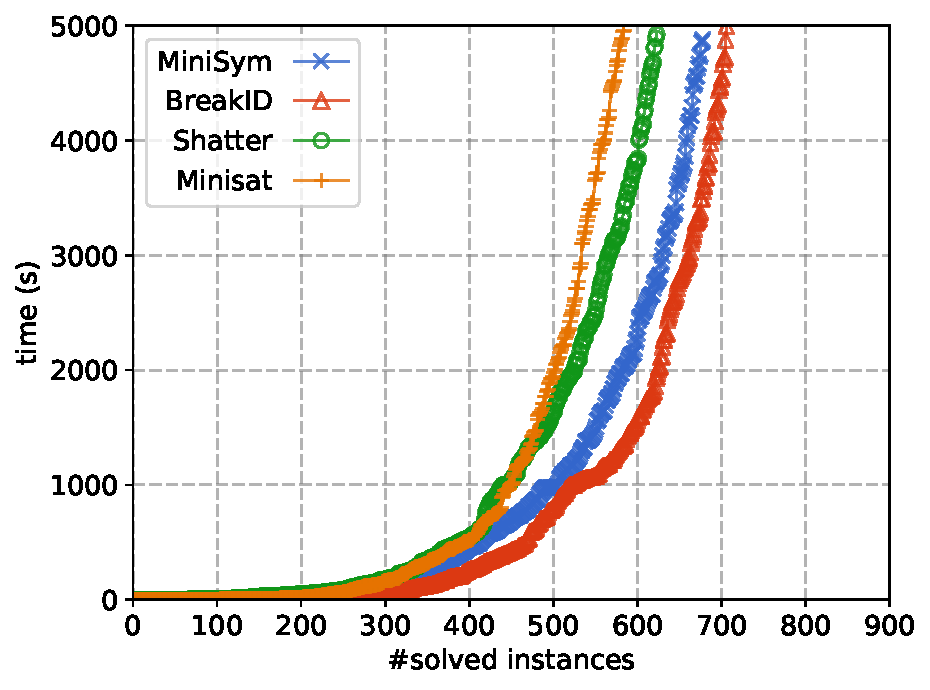
\includegraphics[scale=0.36]{img/saucy-result}}}%
	\qquad
	\subfloat[with \bliss]{{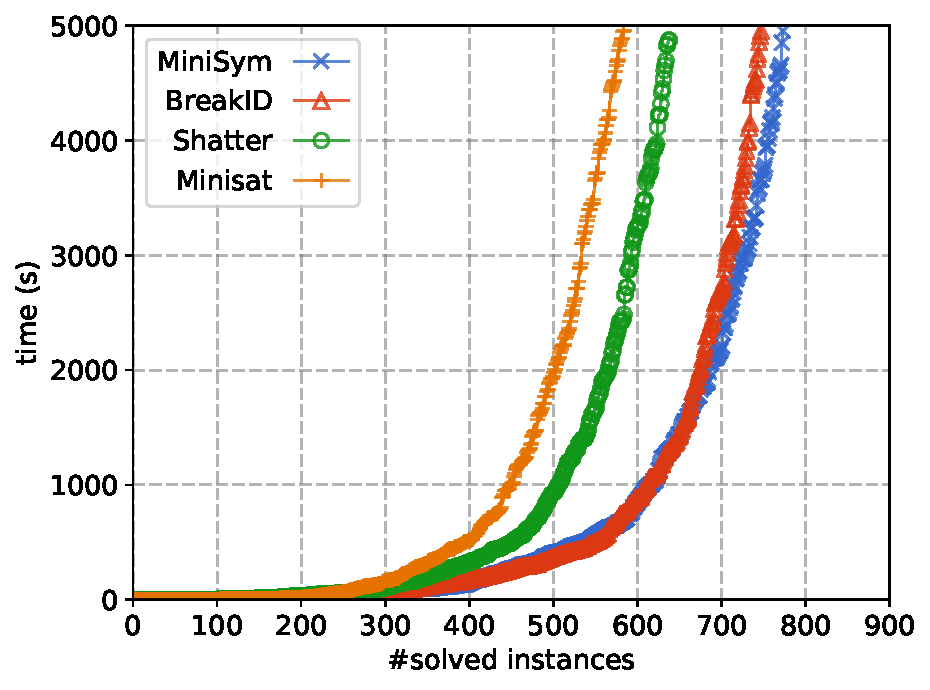
\includegraphics[scale=0.36]{img/bliss-result}}}%
	\caption{Cactus plot  présentant le nombre total d'intances résolues}%
	\label{fig:frcactus}%
\end{figure}

Malgré les très bons résultats obtenus par notre approche, certains problèmes qui sont résolus très 
rapidement par les approches de rupture de symétrie dynamique tel que  Symmetry Propagation (SP) ne pouvaient toujours pas être traité par notre approche et vise-versa.
SP est une approche qui a pour but d'accélérer la traversée de l'espace de recherche en déduisant des faits symétriques à partir des déductions effectuées par le solveur.
À l'inverse notre approche consiste à éliminer les espaces de recherche 
symétriques. %Ces deux approches sont donc orthogonales.
Notre deuxième contribution consiste à déterminer si cette combinaison est possible. Elle se résume donc à la question suivante:
Est-il possible d'accélérer la traversée de l'espace de recherche tout en éliminant les espaces de symétriques ?

Pour que cette approche soit correcte, la contrainte qu'il faut absolument respecter est que la symétrie utilisée pour déduire les
faits symétriques doit être valide dans le problème. En effet, les clauses ajoutées pour éliminer l'espace de recherche
symétrique vont rompre cette symétrie. Cette dernière ne peut donc plus être utilisée pour propager les faits symétriques.
Une approche naïve est de supprimer chacune des symétries dès lors qu'une contrainte de rupture de symétrie a été ajoutée.
Le problème avec cette approche est que l'ensemble vide est très vite atteint et donc que plus aucune déduction symétrique ne peux être faite. Notre approche consiste à traquer les clauses utilisées par le solveur et à connaître à tout instant l'ensemble des symétries valide grâce à l'introduction dite de la notion de symétrie locale pour chaque clause.

\vspace{2em}

\begin{table}[!htbp]\footnotesize
	\centering
	\resizebox{1 \textwidth}{!}{
		\begin{tabular}{l|ccc}
			\toprule
			Benchmark  &\texttt{minisat-Sp} & \texttt{minisat-Sym} & \texttt{minisat-SymSP}\\
			\hline 
			Permutations 0–20 (704) & 194&197&\cellcolor{gray!30,}\textbf{198}\\
			Permutations 20–40 (136) & 33&\cellcolor{gray!30}\textbf{34}&\cellcolor{gray!30}\textbf{34}\\
			Permutations 40–60 (141) & 28&28&\cellcolor{gray!30}\textbf{29}\\
			Permutations 60–80 (168) & \cellcolor{gray!30}\textbf{65}&64&\cellcolor{gray!30}\textbf{65}\\
			Permutations 80–100 (51) & 28&\cellcolor{gray!30}\textbf{34}&\cellcolor{gray!30}\textbf{34}\\
			Permutations  \textgreater100 (200) & 58&59&\cellcolor{gray!30}\textbf{60}\\
			\hline 
			TOTAL no dup (1400) & 406 & 416 & \cellcolor{gray!30,}\textbf{420}\\
			\bottomrule
		\end{tabular}
	}
	\caption{Comparaison des approches sur les instances SAT.}
	\label{tab:satfr}
\end{table}%


\begin{table}[!htbp]\footnotesize
	\centering
	\resizebox{1 \textwidth}{!}{
		\begin{tabular}{l|ccc}
			\toprule
			Benchmark  &\texttt{minisat-Sp} & \texttt{minisat-Sym} & \texttt{minisat-SymSP}\\
			\hline 
			Permutations 0–20 (704) & \cellcolor{gray!30,}\textbf{233}&220&226\\
			Permutations 20–40 (136) & 50&\cellcolor{gray!30}\textbf{54}&\cellcolor{gray!30}\textbf{54}\\
			Permutations 40–60 (141) & 75&\cellcolor{gray!30}\textbf{83}&\cellcolor{gray!30}\textbf{83}\\
			Permutations 60–80 (168) & \cellcolor{gray!30}\textbf{11}&\cellcolor{gray!30}\textbf{11}&10\\
			Permutations 80–100 (51) & \cellcolor{gray!30}\textbf{11}&\cellcolor{gray!30}\textbf{11}&\cellcolor{gray!30}\textbf{11}\\
			Permutations \textgreater100 (200) & 90&\cellcolor{gray!30,}\textbf{109}&107\\
			\hline 
			TOTAL no dup (1400) & 470&488&\cellcolor{gray!30,}\textbf{491}\\
			\bottomrule
		\end{tabular}
	}
	\caption{Comparaison des approches sur les instances UNSAT.}
	\label{tab:unsatfr}
\end{table}

Les expérimentations pour évaluer les performances de l'approche se sont effectuées sur les instances de la SAT Competiton sur sept années 
(2012 - 2018) pour lesquelles $\bliss$ a trouver des symétries. Au total, nous avons obtenu un total de 1400 instances. 
Les tables \ref{tab:satfr} et \ref{tab:unsatfr} présentent respectivement
les résultats obtenues four les problèmes $\sat$ et $\unsat$.
La première colonne de chaque tableau énumère les classes de problèmes sur lesquelles nous avons effectué nos expériences: nous classons les problèmes en fonction du nombre de symétries qu'ils admettent. Une ligne notée $\guillemotleft$permutations X-Y (Z)$\guillemotright$ regroupe les problèmes Z ayant entre X et Y générateurs (symétries). Les autres colonnes indiquent le nombre de problèmes résolus par chaque approche. Les trois solveurs comparés sont respectivement
\texttt{minisat-Sp}, le solveur $\minisat$ avec l'approche SP; \texttt{minisat-Sym} le solveur $\minisat$ avec $\libdsb$ et \texttt{minisat-SymSP} le solveur avec l'approche combiné.
 
Globalement, nous observons que l'approche combinée est efficace dans de nombreuses classes de problèmes symétriques. Pour les problèmes de SAT, la combinaison a de meilleurs résultats que les deux autres approches (4 problèmes de SAT en plus par rapport au meilleur des deux autres). Lorsqu'on examine les problèmes de l'UNSAT, les résultats sont plus mitigés. Cela est du au coût mis en place pour maintenir à jour les structures de chacune des deux approches de manière indépendante.
Cependant l'approche combinée apporte de meilleures résultats dans le nombre total d'instances résolues.

%Cette deuxième contribution réponds à la question, Est-il possible d'accélérer la traversée de l'espace de recherche tout en éliminant l'espace de symétrique ?
%La réponse est positive grâce à l'introduction des symétries locales. 

\chapter*{Abstract}
Nowadays, logic is omnipresent and it is used in different domains such as logic optimization, test pattern generation, formal verification and functional simulation, etc.
One method to solve this kind of problem is satisfiability problem (SAT).
SAT solvers are more and more powerful and can handle large problems which seemed to be infeasible 
few years ago. However, some problems present symmetries which force the solver to explore fruitlessly
the symmetric part of the search space and hinders the performance. 
In this thesis, we set out to exploit symmetry properties of the problems in better ways.
For this purpose, we propose two major contributions that aims to improve the state-of-the-art techniques and augment the number of solved instances. With an evaluation over the instances presented in the SAT competition, we show that our approach overcomes the state-of-the-art ones and is able to solve more instances. 

\newpage
\setcounter{tocdepth}{2}
\tableofcontents

%\newpage
%\listoffigures
%\listoftables

\mainmatter

\chapter{Introduction}\label{chap:intro}

The interest of using computers for logic deduction and reasoning can be traced in the nineteen centuries.
In 1869,  William Stanley Jevons designed and built the first machine doing logic inference.
With the progress of computers, it is used in different domains such as design automation process 
(logic optimization, test pattern generation, formal verification and functional simulation, etc).
Nowadays, one of the methods used in Boolean reasoning is the automatic satisfiability (SAT).
Given a propositional formula (generally the constraints of an encoded problem),
SAT solving consists in deciding whether the formula is satisfiable (i.e., all constraints can be
satisfied) or unsatisfiable (i.e., there is no way to satisfy all constraints at the same time).
This computation is made by a SAT solver that answer $\sat$ when the formula is satisfiable
and $\unsat$ otherwise.
SAT is the first problem that has been proven to be NP-complete in 1971~\cite{cook1971complexity}, this 
means that every NP problem can be solved by encoding it into a SAT one. Solving this problem in 
polynomial time is equivalent to the P versus NP, one of the seven millennium prize problems.

Despite this complexity, SAT solvers are becoming more and more powerful.
Over the last decades, these can handle more and more complex problems in different domains:
like \emph{formal methods} such that: bounded model checking (BMC)~\cite{bmc_99}; \emph{artificial intelligence}: planning decision~\cite{planning_92}; \emph{Informatics} : Haplotype inference~\cite{biology_06}.
In recent work, researchers have succeeded in proving, using a SAT solver, a maximum limit
for the problem of coloring Pythagorean triples~\cite{heule2016solving}, with proof weighing 200 TB.
This success comes from the introduction of sophisticated heuristics and optimization of the solving 
algorithm called Conflict Driven Clause Learning (CDCL) algorithm. It is based on the first non memory
intensive algorithm named by its authors Davis, Putnam, Logemann, and Loveland (DPLL)~\cite{dpll_62}.

Some problems have a huge search space and some of their instances cannot be handled.
An example of such a problem can be the vehicle routing problem (VRP).
It concerns the service of a delivery company, in which
given a fleet of vehicles based in a depot, they must make rounds between several customers  who have requested
each a certain amount of goods. All clients visited by a vehicle refers to the tour of the vehicle. 
The goal is to find the tour that minimizes the delivery cost (monetary, distance, time, …).
Finding the optimal solution for VRP problem is NP-Hard~\cite{toth2002vehicle}.
On an instance of this problem, renaming the set of identical vehicles will give us exactly the same problem.
This is called a \textit{symmetry}. In general, a symmetry is a transformation that leaves an object (or some aspect of the object) unchanged. Symmetries are typically defined as a \textit{syntactical} property of a problem when its presence is inherent to the encoding of the problem. A permutation of variables preserves the original specification. In the case where the symmetries are independent of any 
particular representation of the problem, it is called \textit{semantic}.

The presence of symmetries in a problem leads the search algorithm to fruitlessly explore symmetric
search space and greatly hinders its performance. \textit{Symmetry breaking} is an approach that
avoids the solver to visit symmetric part of the search space. The first step to exploit symmetry is to find them.
In SAT, the detection of syntactical symmetry is done by transforming the specification
in a colored graph and then apply a graph automorphism tool.


%
%This problem leads to combinatorial explosion of the search space.
%
%Different approach have been proposed to to deal with this combinatorial explosion.
%Here, we focus on the exploitation of \textit{symmetries}. 
%
%
%\section{Symmetry}
%
%In general, a symmetry is a transformation that leave an object (or some aspect of the object) unchanged.
%Many problem exhibits symmetry, for example in our previous example renaming a set of identical vehicle,
%rotating a chess board, 
%The presence of symmetry force search algorithm to fruitlessly explore symmetric search space.
%
%
%Symmetries are typically defined as a \textit{syntactical} property of a problem. 
%Its presence is inherent to the encoding of the problem.
%A permutation of variable preserve the original specification. 
%Conversely, a \textit{semantic} symmetries are independent of any 
%particular representation of the problem.
%
%
%To exploit the symmetry of a problem, the first step is to find them.

When symmetries are computed, the most common approach to exploit them is to use a \emph{static symmetry breaking} technique.
It takes the symmetric problem as input and produces a satisfiability equivalent formula by eliminating symmetries. This is done by augmenting the problem with constraints that force the solver to not explore the symmetric search  spaces. It is a easy to integrate static symmetry breaking, no modification of the solver is necessary.
In addition, this approach works well on many symmetric applications.
However, some highly symmetric instances cannot be solved using this technique. Effectively the number of
symmetry breaking constraints can be exponential in relation to the size of the problem and slow down the solver.

Another approach to handle symmetry is \emph{dynamic symmetry breaking}. Here, the management of
symmetries is done during the search. Different approaches exist. First, the behavior of the solver is analyzed to avoid it to visit symmetric part of the search space. Also, some symmetrical facts can be deduced from the
state of the solver. This has the effect of accelerating the tree traversal of the solver and reduce the solving time.

The challenge of this thesis is to understand the state of  the art approach in symmetry breaking and
improve them.
%all constraints of a formula can be satisfiable and answer ,
% or it is not possible to satisfy all constraints and answer \unsat.
%
%The problem of Boolean satisfiability (SAT) is nowadays an unavoidable problem. 
%
%
%
%SAT solving consists in deciding whether 
%all constraints of a formula can be satisfiable and answer \sat, or it is not possible to satisfy all
%constraints and answer \unsat.
%
%
%It consists of deciding whether 
%all constraints of a formula can be satisfiable and answer \sat, or it is not possible to satisfy all
%constraints and answer \unsat.


%
%Nowadays, computers are powerful and used in many applications in different domains.
%One of these domains is critical application that run in planes, cars, trains, etc.
%Software present in these machines must be correct and exempt of bugs.
%Proving the correctness of these software is a difficult problem. 
%
% can leads to combinatorial explosion.
% 
% 
%Over the years, computer scientists have developed many techniques to solve 
%these kinds of problems like \emph{constraint programming} (CP) \cite{rossi2006handbook},
%\emph{Propositional Satisfiability} (SAT) \cite{biere2009handbook},
%\emph{Satisfiability Modulo Theory} (SMT) \cite{barrett2018satisfiability}.
%
%
%
%In this thesis, we focus on solving propositional or Boolean formula, it consists of deciding whether 
%all constraints of a formula can be satisfiable and answer \sat, or it is not possible to satisfy all
%constraints and answer \unsat.
%This problem may appear to be simple but cannot be handled efficiently
%at the moment. This is due to the complexity of the problem which is prove to be NP-complete in 1971. 
%Many industrial applications problems can be transformed into a SAT problem.
%Improving the performance of tools that resolve this problem is an important challenge. 
%
%Over the last decades, SAT solver can handle more and more complicated problems in different domains:
%like \emph{formal methods}: hardware model checking,
%software model checking, etc.; \emph{artificial intelligence}: planning~\cite{planning_92}; \emph{game resolution}:
%sudoku, n-queens, \emph{Bioinformatics} : Haplotype inference,
%\emph{design automation} : equivalence checking.
%A recent work solve the Pythagorean triple, an old mathematical problem which has been resolved with 
%a SAT solver and produce a huge proof of 200 TB.
% 
%This success comes from the introduction of sophisticated heuristics and optimization of the solving 
%algorithm called Conflict Driven Clause Learning (CDCL) algorithm. It is based on the first non memory
%intensive algorithm named by its authors Davis, Putnam, Logemann, and Loveland (DPLL).
%Unfortunately, some problems still intractable for state-of-the-art SAT solvers. But some 
%of them exhibits symmetries that can be exploited by the solver to accelerate the overall solving time.
%At its most basic, symmetry is some transformations of an object that leaves it unchanged.
%Symmetries is common in real life, if we take some butterfly, it has exactly the same halves.
%In the case of satisfiability problems, it maps a solution of a problem to another.
%Ignoring these properties forces the solver to explore equivalent search space and it is a loss of
%time and energy. Considering the butterfly example if we search a pattern and it is not present, it is
%completely absurd to verify the other side. 
%
%In the literature, some works exist and tackle the symmetry problems.
%But, the first step to exploit symmetries is to find them. For this purpose, it exists technique 
%that use graph isomorphism.
%When symmetries are found, the most common approach to exploit it is \emph{static symmetry breaking}.
%It takes the symmetric problem as input and produces a satisfiability equivalent formula without symmetries. This transformation is made without any change of existing solvers. This approach works 
%well on many applications but stuck on some highly symmetrical ones.
%
%Another approach to handle symmetry is \emph{dynamic symmetry breaking}, it is included in the solver. It observes his behavior and use symmetry properties to avoid visiting symmetric search space.
%These approaches will be clearly explained all along this thesis.
%
This thesis addresses the challenge of optimizing the solving of a SAT problem in presence of
symmetries. In detail, my research exploits symmetry breaking during the solving.
%Understanding state-of-the-art techniques allows us to improve it.
Two major contributions are presented. The first one uses the strengths of static symmetry 
breaking approach and applied it dynamically to avoid the drawbacks of the approach. It adds an opportunistic symmetry controller that avoids visiting symmetric part of the search spaces. Benchmarks show that this makes it possible
 to solve very difficult symmetric problems.
The second contribution uses the previous one and combines it with state-of-the-art dynamic 
symmetry breaking approach and so takes the best of two worlds. This combination leads to 
important theoretical step for the usage of \emph{partial symmetry breaking} with the usage of 
\emph{local symmetries}. 
 
%\section{Structure of the manuscript}
The remaining of this document is organized in 6 chapters. Chapter 2 describes the state of
the art for the Boolean satisfiability problem, Chapter 3 focuses on the symmetry present in SAT.
Chapter 4 focuses on the first contribution that uses dynamically the symmetries.
Chapter 5 describes our second proposal and Chapter 6 conclude the thesis. More precisely:
 
\textbf{The Boolean Satisfiability Problem}
The goal of \cref{chap:preliminaries} is to better understand what is SAT. 
It describes in detail the basics
about propositional logic that will be used in the rest of the manuscript. Satisfiability is a hard
problem but some particular forms that are easier to solve such as 2-SAT, Horn SAT and Xor-SAT are presented.
This chapter also describes  the original DPLL algorithm, and the
nowadays used CDCL algorithm and their important points. SAT can nowadays handle
sophisticated problems, thanks to different heuristics.
 An overview of these are presented. Finally, with the presence of multi
core machines, an overview of the state-of-the-art parallel SAT solving are presented.

\textbf{Symmetries and SAT}
The goal of \Cref{chap:symmetryinsat} is to better understand what is a symmetry. 
It requires an understanding of the group theory, and the notation used in the rest of the manuscript.
This chapter also presents the process to find the (syntactic) symmetries of a SAT problem.
 This computation involves the creation of a graph from the problem and the computation of an
automorphism tool. After obtaining the symmetries, the second part presents how to
exploit them for reducing the search space of the solver. The two major approaches that
are the static symmetry breaking approach and the dynamic symmetry breaking approach.
Static symmetry breaking is so far the most popular approach to take advantage of symmetries. It relies on a symmetry preprocessor which augments the initial problem with constraints that force the solver to consider only a few configurations among the many symmetric ones.
Dynamic symmetry breaking exploits the symmetries during the computation of the SAT solver to accelerate the
tree traversal of the SAT solver using symmetrical facts or avoids symmetric configurations like in the 
static approach.
\textbf{Between Static and Dynamic}
\Cref{chap:symmSAT} describes our efficient dynamic symmetry breaking approach.
The first part explains our algorithm, a new way to handle symmetries that avoid the main problem
of the current static approaches. Our proposal has been implemented in state-of-the-art
SAT solver called $\minisat$~\cite{een2003extensible}. The second part presents the extensive experiments on the benchmarks of last six SAT competitions,
which show that our approach is competitive with the best state-of-the-art static symmetry breaking solutions.
The last part presents different heuristics that can improve the performance of our algorithm.

\textbf{Compose dynamic symmetry handling}
\Cref{chap:compose} describes the theoretical and practical aspects of combining two existing
symmetry  breaking approach with the introduction of \textit{local symmetries}.
 An extensive experiments show that the hybrid approach is better than 
each approach individually. The local symmetries allows to combine another 
symmetry breaking approach.
Finally, \Cref{chap:conclu} concludes this manuscript and discusses different directions we have identified for future works.
 
%% Local Variables:
%% TeX-master: "main.tex"
%% ispell-dictionary: "en_US"
%% mode: latex
%% mode: flyspell
%% coding: utf-8
%% End:


\part{State-of-the-art}
% Chapters

\setcounter{mtc}{2} 
\chapter{The Boolean Satisfiability Problem}\label{chap:preliminaries}
\minitoc
In this thesis, our goal is to exploit the symmetry properties of SAT problems.
Before, we get to the heart of the matter, we first introduce the Boolean satisfiability (SAT)  problem.
%This is a propositional formula representing constraints.
%A tool that aims to satisfy such formulas is called a SAT solver. 
%It answers $\sat$ when all constraints
%present in the formula can be satisfied and $\unsat$ otherwise.

\section{SAT basics}
A satisfiability problem is constituted of \emph{Boolean} or \emph{propositional variables},
i.e. each variable has two possible values: true or false (noted respectively $\true$ or $\false$).
We call \emph{literal}, a propositional variable or its negation.
For a given variable $x$, the positive literal is represented by $x$ and the negative one by $\neg x$.
Given a formula $\varphi$, we denote $\Vars_\varphi$ ($\Lits_\varphi$) the set of variables (literals) used in the formula (the index in $\Vars_\varphi$ and $\Lits_\varphi$ is usually omitted when
clear from context).
To build complex formulas, different operators are used, $\neg, \lor$ and $\land$ that are respectively negation, disjunction and conjunction. the remaining operators like, $\Rightarrow, \Leftrightarrow$ and
$\oplus, \cdots$ can be expressed by the use of the basic ones.
For example, $a \Rightarrow b$, can be expressed by $ \neg a \lor b$.
In the absence of parenthesis, the following priority order applies (from the highest to the lowest priority):
negation ($\neg$), conjunction ($\land$), disjunction ($\lor$).

An \emph{assignment}, noted $\alpha$, is defined as the function that assings a value to each variable of $\varphi$.
 $$\alpha: \Vars \mapsto \{ \true, \false \}$$
 As usual, $\alpha$ is said \emph{total}, or \emph{complete}, when all elements of $\Vars$ have an image by
$\alpha$, otherwise it is \emph{partial}. By abuse of notation, an assignment is
often represented by the set of its true literals. For example, $\alpha = \{\neg x_1, x_3 \}$ means that $x_1$
is set to false value and $x_3$ is set to true.
  The set of all (possibly partial) assignments of $\Vars$ is noted $\Assignments(\Vars)$.
A \emph{truth table} gives an evaluation of all possible assignments for a given formula.
\Cref{tab:truthtable} shows the evaluation of the negation ($\neg$), the conjunction ($\land$), and the disjunction ($\lor$) operators.
For convenience, true value (\true) is also represented by $1$, and false value (\false) is represented by $0$.
When a formula is always true, independently from the assignment, it is called a \emph{tautology}: $x \lor \neg x$ is 
an example of tautologous formula.

\begin{table}[!htbp]
 \centering
 \begin{tabular}{cc|ccc}
  $x$ & $y$ & $\neg x$ & $x \lor y$ & $x \land y$ \\
  \toprule
  0 & 0 & 1 & 0 & 0 \\
  \midrule
  0 & 1 & 1 & 1 & 0 \\
  \midrule
  1 & 0 & 0 & 1 & 0 \\
  \midrule
  1 & 1 & 0 & 1 & 1 \\
  \bottomrule
 \end{tabular}
 \caption{Truth table of basic operators}
 \label{tab:truthtable}
\end{table}
\subsection{Normal forms}
In Boolean logic, it exists some structural properties, called \emph{normal form}.
To introduce them, we first need to present the concepts of \emph{cube} and \emph{clause}.
A \emph{cube} $\gamma$ is a finite conjunction of literals represented equivalently by:
$$\gamma = \bigwedge_{i=1}^k l_i $$
A \emph{clause} $\omega$ is a finite disjunction of literals represented equivalently by:
$$\omega = \bigvee_{i=1}^k l_i \text{, or by the set of its literals } \omega = \{l_i\}_{i \in \llbracket 1,k \rrbracket}$$
 
With respect to its size, a clause is said to be \emph{unary, binary, ternary, $n$-ary} if it contains respectively one, two, three, or $n$ literals.
%The clause form has a property called \emph{subsumption}. 
When a clause $\omega_1$ is a subset of another clause $\omega_2$, noted $\omega_1 \subset \omega_2$,
we say thath $\omega_{1}$ subsumes $\omega_{2}$.
 And any assignment that satisfies $\omega_1$ will also satisfy $\omega_2$. So, $\omega_2$ is \emph{redundant} w.r.t. $\omega_1$ and can be removed from the formula.
\emph{Conjunctive Normal Form} (CNF) of a formula is a finite conjunction of clauses represented by
  $$\varphi = \bigwedge_{i=1}^k \omega_i \text{ (or by the set of its clauses } \varphi = \{\omega_i\}_{i \in \llbracket 1,k \rrbracket}\text{)}$$
  
\emph{Disjunctive normal form} (DNF) of a formula is finite disjunction of cubes represented by:
  $$\varphi = \bigvee_{i=1}^k \gamma_i \text{ (or by the set of its cubes } \varphi = \{\gamma_i\}_{i \in \llbracket 1,k \rrbracket}\text{)}$$
The following table is a summary of the laws that allow to transform any formula to
a normal form.
\begin{table}[!htbp]
 \centering
 \begin{tabular}{lllc}
  \multirow{2}{*}{Associativity laws} & $(x \lor y) \lor z \equiv x \lor (y \lor z)$\\
          & $(x \land y) \land z \equiv x \land (y \land z)$\\
  \hline              
  \multirow{2}{*}{Commutativity laws} & $x \lor y \equiv y \lor x$\\
          & $x \land y \equiv y \land x$\\
  \hline      
  \multirow{2}{*}{Identity laws} & $x \lor \false \equiv x$\\
           & $x \land \true \equiv x$\\
  \hline        
  \multirow{2}{*}{Domination laws} & $x \lor \true \equiv \true$\\
           &  $x \land \false \equiv \false$\\
  \hline        
  \multirow{2}{*}{Idempotent laws} & $x \lor x \equiv x$\\
               & $x \land x \equiv x$\\     
  \hline        
  \multirow{2}{*}{Distributive laws} & $x \lor (y \land z) \equiv (x \lor y) \land (x \lor z)$\\
           & $x \land (y \lor z) \equiv (x \land y) \lor (x \land z)$\\
 \hline        
 \multirow{2}{*}{Negation laws}  & $x \lor \neg x \equiv \false$\\
        & $x \land \neg x \equiv \true$\\
  \hline
   double negation law & $\neg (\neg x) \equiv x$ \\
  \hline
  \multirow{2}{*}{De Morgan's laws} & $\neg x \lor \neg y \equiv \neg (x \land y)$\\
            &  $\neg x \land \neg y \equiv \neg (x \lor y)$\\
 \end{tabular}
 \caption{Set of laws of operators}
 \label{tab:laws}
\end{table}
Every formula can be transformed into a normal form with different complexity and the resulting formula is 
\emph{equivalent}.  
In other words, every assignment $\alpha$ that satisfies formula $\varphi$  also models the resulting formula $\psi$
and vice-versa, denoted by $\varphi \equiv \psi$.
 Also, we say a formula $\psi$ is a \emph{logical consequence} of a formula $\varphi$ is every model of $\varphi$
 is also a model of $\psi$ and is denoted by $\varphi \models \psi$.
Conjunctive normal form is the input form of state-of-the-art solvers. Any propositional
formula can be transformed in CNF form with polynomial time. Conversely, DNF form have
an exponential memory complexity during the transformation.
Note that each cube in the problem in DNF form is a solution in the equivalent CNF formulas.
%\hakan{Sharp SAT = transform CNF to DNF}
%A formula is said to be \emph{satisfiable} (\sat) if there is at least one assignment that satisfies it;
%otherwise the formula is \emph{unsatisfiable} (\unsat).
%\subsection{Satisfiability problem}
%A \emph{Boolean variable}, or \emph{propositional variable}, is a variable that
%has two possible values : true or false (noted respectively $\true$ or $\false$).
%A \emph{literal} $l$ is a propositional variable or its
%negation. For a given variable $x$, the positive literal is represented by $x$
%and the negative one by $\neg x$.
%
%A \emph{clause} $\omega$ is a finite disjunction of literals represented
%equivalently by $\omega = \bigvee_{i=1}^k l_i$ or the set of its literals
%$\omega = \{l_i\}_{i \in \llbracket 1,k \rrbracket}$. A clause with a single
%literal is called \emph{unit clause}.
%A clause is a \emph{tautology} if it is always true, a clause that contains a positive 
%and negative value of a clause for example.
%A \emph{conjunctive normal form (CNF) formula} $\varphi$ is a finite
%conjunction of clauses.  A CNF can be either noted $\varphi = \bigwedge_{i=1}^k
%\omega_i$ or $\varphi = \{\omega_i\}_{i \in \llbracket 1,k \rrbracket}$. We
%denote $\Vars_\varphi$ ($\Lits_\varphi$) the set of variables (literals) used in
%$\varphi$ (the index in $\Vars_\varphi$ and $\Lits_\varphi$ is usually omitted when
%clear from context).
%For a given formula $\varphi$, an \emph{assignment} of the variables of
%$\varphi$ is a function $\alpha: \Vars \mapsto \{ \true, \false \}$.  As usual, $\alpha$ is
%\emph{total}, or \emph{complete}, when all elements of $\Vars$ have an image by
%$\alpha$, otherwise it is \emph{partial}. By abuse of notation, an assignment is
%often represented by the set of its true literals.  The set of all (possibly
%partial) assignments of $\Vars$ is noted $\Assignments(\Vars)$.
%The assignment $\alpha$ \emph{satisfies} the clause $\omega$, denoted $\alpha
%\models \omega$, if $\alpha \cap \omega \neq \emptyset$. Similarly, the assignment
%$\alpha$ satisfies the propositional formula $\varphi$, denoted $\alpha \models
%\varphi$, if $\alpha$ satisfies all the clauses of $\varphi$. Note that a
%formula may be satisfied by a partial assignment. In this case, unassigned variable is called
%\emph{don’t care}.
%A formula is said to be
%\emph{satisfiable} (\sat) if there is at least one assignment that satisfies it;
%otherwise the formula is \emph{unsatisfiable} (\unsat).
\subsection{An NP-complete problem}
The SAT problem is the first NP-complete problem proven by Stephen Cook in 1971~\cite{cook1971complexity}.
NP-completeness means that a SAT problem can be solved with a non-deterministic Turing machine in polynomial time (NP) and is also NP-hard. A problem is said NP-hard if everything in NP can be transformed into it in polynomial time. 
One of the most important unsolved problems in theoretical computer science is the P versus NP problem.
This question is one of the seven millennium prize problems.

\subsection{Particular forms easy to solve}
In some particular forms, SAT problems can be computed with polynomial algorithm.

\textbf{2-SAT~\cite{aspvall1979linear}.}
In this particular form, the given CNF formula contains only binary clauses.
In this case, it suffices to create a graph in which each clause is transformed into implication. For example, the clause $x \lor y$ will be transformed into $ \neg x \Rightarrow y,
\neg y \Rightarrow x$. After computing \emph{strong connected component} on this graph, to be looking for
 the positive and negative forms of the same variable, in the same  strong connected component suffices 
to determine the satisfiability of the formula. If it is the case, the formula is \unsat. Otherwise 
a solution can be deduce and the problem is \sat. This algorithm can be computed in linear time complexity.
\textbf{Horn SAT.} In this particular form, the given CNF formula contains only Horn clauses. It exists three form
of Horn clause: \emph{strict Horn clause} that contains only one positive literal and at least one negative literal,
\emph{positive Horn clause} that contains only one positive literal and no negative literals
\emph{negative Horn clause} that contains only negative literals.
To solve this particular form of formula, it suffices to  apply \emph{Boolean constraint propagation} (BCP) or \emph{unit propagation} explained thereafter in \cref{sec:dpll} until fix point.
Roughly speaking, it satisfies all unit clauses in cascades. Either an empty clause was deduced and the problem
is \unsat or the fix point is reached and the formula is \sat. Like 2-SAT, this algorithm can also be computed
in linear time complexity.

\textbf{XOR SAT.} In this particular form, each clause contains xor ($\oplus$) operator rather than or ($\lor$).
This problem can be seen as a system of linear equations. Gaussian elimination allows to solve this kind of
problem is polynomial time.
The membership of polynomial class (P) of the particular form of satisfiability problems describes above is a special case of Schaefer's dichotomy theorem~\cite{schaefer1978complexity}.
\subsection{Some related problems}
Different kind of problems related to SAT is presented is this section.
One of them is sharp-SAT (\#SAT), its purpose is to count the number of solutions in a CNF.

Another related problem is maximum satisfiability problem (MAX-SAT). In this case, the problem
is to find the maximum subset of clauses that can be satisfied for a formula. Different variants
of this problem exist. For example, some constraints must be satisfied (hard clauses) and MAX-SAT
is applied on the remaining clauses called \emph{soft} clauses.
The last related problem is quantified Boolean formula (QBF) where the quantifiers $\exists$ and
$\forall$ are present in the formula. For example, $\forall x\, \exists y\, \exists z \, (x \lor y) \land z$.
This particular form is a generalization of the SAT problem with PSPACE complexity.
\subsection{Solving a SAT problem}
Two kinds of algorithms exist to solve satisfiability problems.
First, the \emph{incomplete} algorithm~\cite{kautz2009incomplete} which does not provide any guarantee that will eventually report either any satisfiable assignment or declare the formula unsatisfiable. This kind of algorithm is out of scope of this thesis. 
Second, the \emph{complete} algorithm, which provides a guarantee that if an assignment exists
it will be reached or it will declare that formula is unsatisfiable.
This section describes different \emph{complete }algorithm to solve a propositional formula.
\subsubsection{A naive algorithm}
A naive approach to solve a SAT problem is to try all possible assignments.
For a propositional formula with $n$ variables, it leads to $2^n$ assignments in the worse case.  
\Cref{fig:naive_algo} illustrates the search tree for a given problem with six variables.
The presented formula in the figure has 6 clauses, with 2 ternary clauses and 4 binary clauses.
It will be used as an example in different algorithm presented below. This formula is $\sat$,
$\alpha_{11} = \{\neg x_1, \neg x_2, x_3, \neg x_4, x_5, \neg x_6 \}$ is a solution of the problem.
This naive algorithm will check 10 assignments before finding the solution. 
In the general case, due to the number of variables in problems, this algorithm is intractable.
\begin{figure}[!htbp]
 \centering
 
\begin{minipage}[c]{0.6\linewidth}
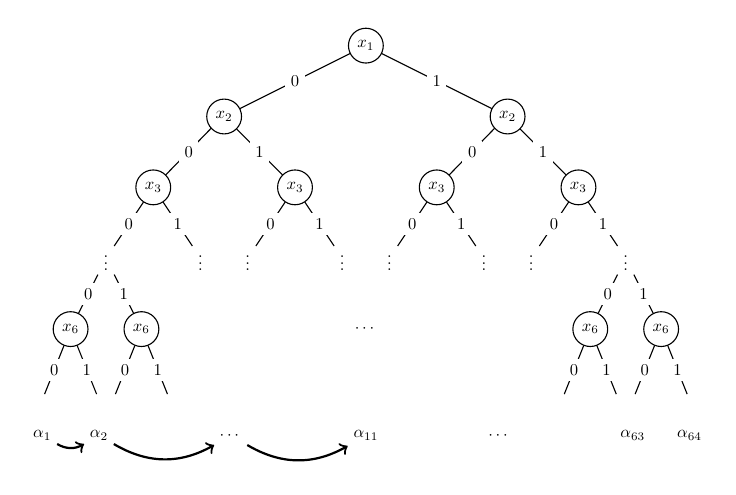
\begin{tikzpicture}[level/.style={sibling distance=60mm/#1},every node/.style={scale=0.6}, scale=0.6]
  \tikzstyle{trans}=[thick, ->, sloped]

\node [circle,draw] (x1) {$x_1$}
  child {node [circle,draw] (x2_1) {$x_2$}
    child {node [circle,draw] (x3_1) {$x_3$}
      child {node  (xn_1) {$\vdots$}
        child {node [circle,draw] (x6_1) {$x_6$}
        	child {node (x6_1f) {}
        	child[level distance=0.75cm] { node (a1) {$\alpha_1$} edge from parent[draw=none]}
        }
       		child {node (x6_1t) {}
       			child[level distance=0.75cm] { node (a2) {$\alpha_2$} edge from parent[draw=none]}
         }}
        child {node [circle,draw] (x6_2) {$x_6$}
        		child {node (x6_2f) {}}
        				child {node (x6_2t) {}
        	}
        }
      } 
      child {node (xn_2) {$\vdots$}}
    }
    child {node [circle,draw] (x3_2) {$x_3$}
      child {node (xn_3) {$\vdots$}}
      child {node (xn_4) {$\vdots$}}
    }
  }
  child {node [circle,draw] (x2_2) {$x_2$}
    child {node [circle,draw] (x3_3) {$x_3$}
      child {node (xn_5) {$\vdots$}}
      child {node (xn_6) {$\vdots$}}
    }
  child {node [circle,draw] (x3_4) {$x_3$}
    child {node (xn_7) {$\vdots$}}
    child {node (xn_8) {$\vdots$}
      child {node [circle,draw] (x6_3) {$x_6$}
      	       child {node (x6_3f) {}}
      	child {node (x6_3t) {}
        }}
      child {node [circle,draw] (x6_4) {$x_6$}
      	child {node (x6_4f) {}
        child[level distance=0.75cm] { node (an_1) {$\alpha_{63}$} edge from parent[draw=none]}
    	}
	    child {node (x6_4t) {}
    		child[level distance=0.75cm] { node (an) {$\alpha_{64}$} edge from parent[draw=none]}
      }}}
  }
};

\path (x6_2) -- (x6_3) node (x) [midway] {$\cdots$}
        child[level distance=2.25cm] { node (a_11) {$\alpha_{11}$} edge from parent[draw=none]};


\path (a2) -- (a_11) node (b1) [midway] {$\cdots$};
\path (a_11) -- (an_1) node (b2) [midway] {$\cdots$};

\draw[trans] (a1) to [bend right]  (a2);
\draw[trans] (a2) to [bend right]  (b1);
\draw[trans] (b1) to [bend right]  (a_11);

% to [bend right]  (b1) to [bend right]  (a_11);

\path (x1)   -- (x2_1) node [midway, fill=white] {$0$};
\path (x2_1) -- (x3_1) node [midway, fill=white] {$0$};
\path (x3_1) -- (xn_1) node [midway, fill=white] {$0$};
\path (xn_1) -- (x6_1) node [midway, fill=white] {$0$};
\path (x3_2) -- (xn_3) node [midway, fill=white] {$0$};
\path (x2_2) -- (x3_3) node [midway, fill=white] {$0$};
\path (x2_2) -- (x3_4) node [midway, fill=white] {$1$};
\path (x1)   -- (x2_2) node [midway, fill=white] {$1$};
\path (xn_1) -- (x6_2) node [midway, fill=white] {$1$};
\path (x3_1) -- (xn_2) node [midway, fill=white] {$1$};
\path (x2_1) -- (x3_2) node [midway, fill=white] {$1$};
\path (x3_2) -- (xn_4) node [midway, fill=white] {$1$};
\path (x3_3) -- (xn_5) node [midway, fill=white] {$0$};
\path (x3_3) -- (xn_6) node [midway, fill=white] {$1$};
\path (x3_4) -- (xn_7) node [midway, fill=white] {$0$};
\path (x3_4) -- (xn_8) node [midway, fill=white] {$1$};
\path (xn_8) -- (x6_3) node [midway, fill=white] {$0$};
\path (xn_8) -- (x6_4) node [midway, fill=white] {$1$};


\path (x6_1) -- (x6_1f) node [midway, fill=white] {$0$};
\path (x6_1) -- (x6_1t) node [midway, fill=white] {$1$};

\path (x6_2) -- (x6_2f) node [midway, fill=white] {$0$};
\path (x6_2) -- (x6_2t) node [midway, fill=white] {$1$};

\path (x6_3) -- (x6_3f) node [midway, fill=white] {$0$};
\path (x6_3) -- (x6_3t) node [midway, fill=white] {$1$};

\path (x6_4) -- (x6_4f) node [midway, fill=white] {$0$};
\path (x6_4) -- (x6_4t) node [midway, fill=white] {$1$};

\end{tikzpicture}
\end{minipage}
\begin{minipage}[c]{0.23\linewidth}
           \footnotesize
		\begin{itemize}
			\item[] $\omega_1 = \{x_1, x_2, x_3\}$ 
			\item[] $\omega_2 = \{x_4, x_5, x_6\}$
			\item[] $\omega_3 = \{\neg x_1, \neg x_5\}$
			\item[] $\omega_4 = \{\neg x_2, \neg x_4\}$
			\item[] $\omega_5 = \{\neg x_3, \neg x_4\}$
			\item[] $\omega_6 = \{\neg x_3, \neg x_6\}$
		\end{itemize}
\end{minipage}

 \caption{All possible assignments for a problem with 6 variables}
 \label{fig:naive_algo}
\end{figure}
\subsubsection{Davis Putnam Logemann Loveland algorithm (DPLL)}\label{sec:dpll}
One of the first non-memory-intensive algorithm developed to solve SAT problems is 
the Davis Putnam Logemann Loveland algorithm (DPLL)~\cite{dpll_62}. 
It explores a binary tree using depth first search as shown in \Cref{algo:dpll}.
The construction of the tree  relies on the \emph{decision} made (on \cref{algo:dpll:decision}). Both values
are checked, true value on \cref{algo:dpll:pos} and false value on \cref{algo:dpll:neg}.
When a leaf find a conflict (\cref{algo:dpll:unsatbranch}) which means that the formula cannot be satisfied with
the current assignment, other branches are explored.
By recursive construction of the algorithm, when each value of a literal reach to a conflict,
solver \emph{backtracks} at most one level, this fact is called \emph{chronological backtracking}.
When the conflict occurs at the top of the tree, it means that the formula cannot be satisfied and the 
solver reports $\unsat$ (\cref{algo:dpll:unsat}). However, if the formula is empty in any branch, 
it means that current assignment satisfy the whole formula and the solver reports it on \cref{algo:dpll:sat1}
or \ref{algo:dpll:sat2}.
\begin{algorithm}[!htbp]
	\SetKwProg{Fn}{function}{}{}
	\SetKwFunction{DPLL}{DPLL}	
	\SetKwFunction{unitPropagation}{unitPropagation}
	\SetKwFunction{purePropagation}{purePropagation}
	\SetKwFunction{assignDecisionLiteral}{assignDecisionLiteral}

	
	\Fn{
		\DPLL{$\varphi$: CNF formula, $\alpha$ assignment}\\
		$\quad\quad$\textbf{returns} an assignment if $\varphi$ is \sat and $\unsat$ otherwise
	}
	{	
		$\varphi, \alpha \gets$ \unitPropagation{$\varphi, \alpha$}\;
	\label{algo:dpll:unit}
		\If{$\{\} \in \varphi$}{\Return \false \tcp*{Conflict}}	 \label{algo:dpll:unsatbranch}
		
		\If{$\varphi = \{\}$}{\Return $\alpha$ \tcp*{$\varphi$ is $\sat$}}
		
		$x \gets$ \assignDecisionLiteral{}\; \label{algo:dpll:decision}

		\If{$\alpha \gets$ \DPLL{$\varphi \cup \{x\}, \alpha $} \label{algo:dpll:pos}} 
		{
			\Return $\alpha$ 		\label{algo:dpll:sat1}
		}
		\If{ $\alpha \gets$ \DPLL{$\varphi \cup \{\neg x\}, \alpha $} \label{algo:dpll:neg}}
		{
			\Return $\alpha$ 		\label{algo:dpll:sat2}
		} 
	
		\Return \unsat \tcp*{$\varphi$ is $\unsat$}\label{algo:dpll:unsat}
	}
	\caption{The DPLL algorithm.}
	\label{algo:dpll}
	
\end{algorithm}
An important function in the DPLL algorithm is \texttt{unitPropagation} (\cref{algo:dpll:unit}).
It is presented in \Cref{algo:unitdpll}. This function set value to unit clause in order to satisfy them
until fix point is reached. Either, there
 are no more unit clause in the formula or an inconsistency 
is found which means that current assignment cannot satisfy the formula. In the later case, the solver will
backtrack and another branch will be explored.
\begin{algorithm}[!htbp]
	\SetKwProg{Fn}{function}{}{}
	\SetKwFunction{unitPropagation}{unitPropagation}
	\Fn{
		\unitPropagation{$\varphi$: CNF formula, $\alpha$ assignment}\\
		$\quad\quad$\textbf{returns}  CNF formula and assignment $\alpha$ 
	}
	{	
		\While{$\{l\} \in \varphi$ \textbf{and} $\{\} \notin \varphi$  }
		{
			\tcp{\small Remove all clauses containing $l$, all literals $\neg l$}
			$\varphi \gets \varphi\mid_{\,l}$\\
			$\alpha \gets \alpha \cup \{l\}$

		}
	\Return $\varphi, \alpha$
	}
	\caption{Unit propagation}
	\label{algo:unitdpll}
	
\end{algorithm}
When DPLL algorithm is executed on the formula of \Cref{fig:naive_algo}, after making decisions on literals
$\neg x_1$ and $\neg x_2$, unit propagation detects that $x_3$ must be assigned to true.
This propagation prevents to explore  multiple assignments. Effectively, when $x_3$ is set to false value,
the clause $\omega_1$ is not satisfied and it remains 3 variables and so $2^3$ possible assignments
(from $\alpha_1$ to $\alpha_8$) are discarded.
Moreover, in the DPLL algorithm, application of unit propagation until the fix point is reached leads  to a solution.
\texttt{assignDecisionLiteral} is an important procedure that responsible of choosing the variable that
divides the search space. Its objective is to find a literal that will generate a maximum of unit propagations. Intuitively, decision literals can be viewed as ‘guesses’ and propagated literals can be viewed as ‘deductions’. 
Finding a optimal variable is NP-Hard. Different heuristics exists to choose the decision variable,
some of them will be presented in the section~\ref{sec:heuristics}.
%\input{algo/puredpll}
%Another idea introduced by DPLL was \emph{elimination of pure literals},
%a literal is said pure if it only appear on one sign (positive or negative) in the problem.
%These literals are set to true in the assignment.
%On consequence, all clauses that own these literals are satisfied and so can be removed.
%
\subsubsection{Conflict Driven Clause Learning (CDCL) algorithm}\label{sec:cdcl}
The principal weakness of DPLL algorithm is to make the same inconsistencies several times
(principally due to chronological backtracking), leading to  unnecessary CPU usage.\\
Conflict Driven Clause Learning (CDCL) \cref{algo:cdcl} is a sound and complete algorithm
that overcomes the weakness of DPLL.
\Cref{algo:cdcl} gives an overview of CDCL, Like DPLL,  it walks on a binary search tree.
Initially, the  assignment is empty and the decision level that 
indicates the depth of the search tree, noted by $dl$, is set to zero.
The algorithm first applies unit propagation to the formula $\varphi$ for the  assignment $\alpha$ (\cref{alg:cdcl:unit}).
%Note that it is  the same procedure as the one used for DPLL.
An inconsistency or a \emph{conflict} at level zero indicates that the formula is unsatisfiable, and the algorithm
reports it (from \cref{alg:cdcl:unsat_start} to \cref{alg:cdcl:unsat_end}). When the conflict is occurring at a higher level, its reason is analyzed and a clause called \emph{conflict clause} is deduced (\cref{alg:cdcl:analyze}).
The work done in this procedure will be explained thereafter.
This clause is \emph{learnt} (\cref{alg:cdcl:learn}) (added to the formula). This clause is redundant w.r.t the current
formula and so it does not change the satisfiability of $\varphi$. It also avoids encountering a conflict with the same
causes in the future.
The analysis is completed by the computation of a \emph{backjumps level} , the assignment and decision level is updated (\cref{alg:cdcl:backjump}). As the level can be much lower than the level of the current assignment, this is called \emph{non-chronological backtracking}.
Finally, if no conflict appears, the algorithm chooses a new decision literal 
(\cref{alg:cdcl:pick_start,alg:cdcl:pick_end}).
The above steps are repeated until the satisfiability status of the
formula is determined.
\begin{algorithm}
	\SetKwProg{Fn}{function}{}{}
	\SetKwFunction{CDCL}{CDCL}
	\SetKwFunction{unitPropagation}{unitPropagation}
	\SetKwFunction{analyzeConflict}{analyzeConflict}
	\SetKwFunction{addLearntClause}{addLearntClause}
	\SetKwFunction{assignNewLiteral}{assignDecisionLiteral}
	\SetKwFunction{backjumpPolicy}{backjumpAndRestartPolicies}
	\SetKwFunction{ca}{currenttAssignment}
	\Fn{
		\CDCL{$\varphi$: CNF formula}\\
		$\quad\quad$\textbf{returns} $\true$ if $\varphi$ is \sat and $\false$ otherwise
	}
	{
		$dl \gets 0$ \tcp*{Current decision level}
		$\alpha \gets \emptyset$\;
		\While{not all variables are assigned}{
			$\varphi, \alpha \gets$ \unitPropagation{$\varphi|_\alpha, \alpha$}\;\label{alg:cdcl:unit}
			\If(\tcp*[f]{A conflict occurs}){ $\{\} \in \varphi$}
			{ 
				\If{dl = 0}{\label{alg:cdcl:unsat_start} 
					\Return \false \label{alg:cdcl:unsat_end} 
					\tcp*{$\varphi$ is $\unsat$}
				}
				$\omega \gets$ \analyzeConflict{}\;\label{alg:cdcl:analyze} 
				$dl \gets$ \backjumpPolicy{}\;\label{alg:cdcl:backjump} 
				$\varphi \gets \varphi \cup \{\omega$\} \; \label{alg:cdcl:learn}
				
			}
			\Else{
				$\alpha \gets \alpha\, \cup $ \assignNewLiteral{}\; \label{alg:cdcl:pick_start} 
				$dl \gets dl+1$\;\label{alg:cdcl:pick_end} 
			}
		}
		\Return \true
		\tcp*{$\varphi$ is $\sat$}
	}
	\caption{The CDCL algorithm.}
	\label{algo:cdcl}
	
\end{algorithm}
\subsection{Conflict Analysis}
A conflict is an inconsistency discovered by the solver, a situation that requires for a variable to be set 
simultaneously to the \true and \false values. \Cref{fig:conflict} shows an assignments that leads to a conflict.
First the solver chooses $\neg x_1$ as a decision (marked with a D in the figure) then, $\neg x_6$ and, then $\neg x_5$. This last one propagates $x_4$ (marked with aa P in the figure),
which in turn propagates $x_2$ and $x_3$.
To satisfy $\omega_1$, $x_3$ needs to be set to $\true$ and  to satisfy $\omega_5$, 
needs to be $\false$. As a variable cannot have both values, a conflict appears (marked as a C in the figure).
\begin{figure}[!htbp]
 \centering
  {\scriptsize
\newcommand{\ratioc}{0.195}
%\begin{minipage}[l]{\ratioc\linewidth}
%	\begin{itemize}
%		\item[] $\omega_1 = \{\cred{x_1}, x_2, x_3\}$ 
%		\item[] $\omega_2 = \{x_4, x_5, x_6\}$
%		\item[] $\cgreen{\omega_3} = \{\cgreen{\neg x_1}, \neg x_5\}$
%		\item[] $\omega_4 = \{\neg x_2, \neg x_4\}$
%		\item[] $\omega_5 = \{\neg x_3, \neg x_4\}$
%		\item[] $\omega_6 = \{\neg x_3, \neg x_6\}$
%	\end{itemize}
%\end{minipage}
\begin{minipage}[b]{\ratioc\linewidth}
	\begin{itemize}
	\item[] $\omega_1 = \{\cred{x_1}, x_2, x_3\}$ 
	\item[] $\omega_2 = \{x_4, x_5, \cred{x_6\}}$
	\item[] $\cgreen{\omega_3} = \{\cgreen{\neg x_1}, \neg x_5\}$
	\item[] $\omega_4 = \{\neg x_2, \neg x_4\}$
	\item[] $\omega_5 = \{\neg x_3, \neg x_4\}$
	\item[] $\cgreen{\omega_6} = \{\neg x_3, \cgreen{\neg x_6\}}$
\end{itemize}
\end{minipage}
\begin{minipage}[b]{\ratioc\linewidth}
		\begin{itemize}
		\item[] $\omega_1 = \{\cred{x_1}, x_2, x_3\}$ 
		\item[] $\omega_2 = \{\cprop{x_4}, \cred{x_5}, \cred{x_6\}}$
		\item[] $\cgreen{\omega_3} = \{\cgreen{\neg x_1}, \cgreen{\neg x_5\}}$
		\item[] $\omega_4 = \{\neg x_2, \neg x_4\}$
		\item[] $\omega_5 = \{\neg x_3, \neg x_4\}$
		\item[] $\cgreen{\omega_6} = \{\neg x_3, \cgreen{\neg x_6\}}$
	\end{itemize}
\end{minipage}
\begin{minipage}[b]{\ratioc\linewidth}
			\begin{itemize}
		\item[] $\omega_1 = \{\cred{x_1}, x_2, x_3\}$ 
		\item[] $\cgreen{\omega_2} = \{\cgreen{x_4}, \cred{x_5}, \cred{x_6\}}$
		\item[] $\cgreen{\omega_3} = \{\cgreen{\neg x_1}, \cgreen{\neg x_5\}}$
		\item[] $\omega_4 = \{\neg x_2, \cred{\neg x_4}\}$
		\item[] $\omega_5 = \{\neg x_3, \cred{\neg x_4}\}$
		\item[] $\cgreen{\omega_6} = \{\neg x_3, \cgreen{\neg x_6\}}$
	\end{itemize}
\end{minipage}
\begin{minipage}[b]{\ratioc\linewidth}
	\begin{itemize}
		\item[] $\omega_1 = \{\cred{x_1}, x_2, x_3\}$ 
		\item[] $\cgreen{\omega_2} = \{\cgreen{x_4}, \cred{x_5}, \cred{x_6\}}$
		\item[] $\cgreen{\omega_3} = \{\cgreen{\neg x_1}, \cgreen{\neg x_5\}}$
		\item[] $\omega_4 = \{\neg x_2, \cred{\neg x_4}\}$
		\item[] $\omega_5 = \{\neg x_3, \cred{\neg x_4}\}$
		\item[] $\cgreen{\omega_6} = \{\neg x_3, \cgreen{\neg x_6\}}$
	\end{itemize}
\end{minipage}
\begin{minipage}[b]{\ratioc\linewidth}
	\begin{itemize}
		\item[] $\omega_1 = \{\cred{x_1}, \cred{x_2}, \cblue{x_3}\}$ 
		\item[] $\cgreen{\omega_2} = \{\cgreen{x_4}, \cred{x_5}, \cred{x_6\}}$
		\item[] $\cgreen{\omega_3} = \{\cgreen{\neg x_1}, \cgreen{\neg x_5\}}$
		\item[] $\cgreen{\omega_4} = \{\cgreen{\neg x_2}, \cred{\neg x_4}\}$
		\item[] $\omega_5 = \{\cblue{\neg x_3}, \cred{\neg x_4}\}$
		\item[] $\cgreen{\omega_6} = \{\neg x_3, \cgreen{\neg x_6\}}$

	\end{itemize}
\end{minipage}
}


 \caption{Decisions/Propagations that leads to a  conflict}
 \label{fig:conflict}
\end{figure}
This series of decisions would provoke same propagation and leads to the same conflict. To escape this
situation, the solver needs to analyze the reason of the conflict with so-called \emph{implication graph}.
It represents the current state of the solver and so records all dependencies between  variables. It is updated either when a variable is assigned on decision/propagation, or  when a variable
is unassigned (on backjump's operation). The implication graph is a directed acyclic graph (DAG) in which a vertex represents an assigned variable labeled by $l@dl(l)$ where $l$ represents assigned literal and $dl(l)$ represents the decision level of the literal $l$.
Root vertices , that have no incoming edges, represent decision literal. The remaining vertices represent
propagations.
Each incoming arc, labeled with a clause represents the \emph{reason} of this propagation.
This clause must be assertive (i.e. all  literals are false except one that is not yet assigned).
\Cref{fig:implication-graph} shows the implication graph of the previous example (\Cref{fig:conflict}).
\begin{figure}[!htbp]
 \centering
 
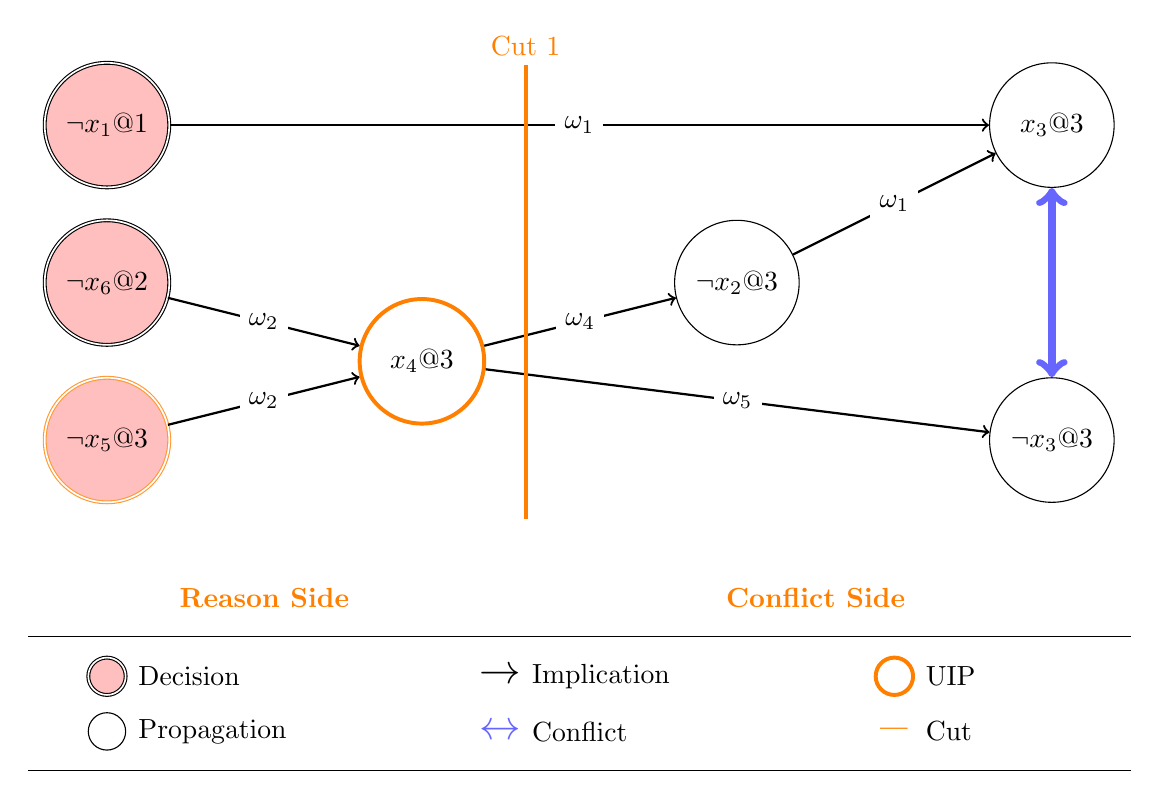
\begin{tikzpicture} % [level/.style={sibling distance=60mm/#1},every node/.style={scale=0.89}, scale=0.89]

	\tikzstyle{decision}=[draw,double,circle,fill=red!25,minimum size=45pt,inner sep=0pt]
	\tikzstyle{propagation}=[draw,circle,fill=white!25,minimum size=45pt,inner sep=0pt]
	
	\node[decision] (dx1) {$\neg x_1$@1};
	\node[decision] (dx6) at ($(dx1) + (0, -2)$) {$\neg x_6$@2};
	\node[decision, draw=orange!80] (dx5) at ($(dx6) + (0, -2)$) {$\neg x_5$@3};
	
	\node[propagation, draw=orange, line width=0.5mm] (px4) at ($(dx6) + (4, -1)$) {$x_4$@3};
	\node[propagation] (px3) at ($(dx5) + (12, 0)$) {$\neg x_3$@3};
	\node[propagation] (px2) at ($(dx6) + (8, 0)$) {$\neg x_2$@3};

	\node[propagation] (px33) at ($(dx5) + (12, 4)$) {$x_3$@3};


	\node[font=\bfseries] (reason) at (2,-6) {\textcolor{orange}{Reason Side}};
	\node[font=\bfseries] (reason) at (9,-6) {\textcolor{orange}{Conflict Side}};

	\path[->, draw, thick] (dx6) -- (px4) node [midway, fill=white] {$\omega_2$};
	\path[->, draw, thick] (dx5) -- (px4) node [midway, fill=white] {$\omega_2$};
	
	\path[->, draw, thick] (px4) -- (px3) node [midway, fill=white] {$\omega_5$};
	\path[->, draw, thick] (px4) -- (px2) node [midway, fill=white] {$\omega_4$};
	
	\path[->, draw, thick] (dx1) -- (px33) node [midway, fill=white] {$\omega_1$};
	\path[->, draw, thick] (px2) -- (px33) node [midway, fill=white] {$\omega_1$};
	\path[<->, draw, line width=1mm, color=blue!60] (px3) -- (px33);
	\path[line width=0.5mm, draw=orange] ($(px4.east) + (0.5, -2)$) -- ($(px4.east) + (0.5, 4)$)  
			   node [fill=white] {\textcolor{orange}{Cut 1}};
	
%	\path[line width=0.5mm, draw=orange!60] ($(px4.east) + (-3.5, -2)$) -- ($(px4.east) + (-3.5, 4)$)
%			   node [fill=white] {\textcolor{orange!70}{Cut 2}};
	
	% Legend
	
	\path[draw] (-1, -6.5) -- (13, -6.5);
	\node[decision, scale=0.3] (ld) at (0, -7) {};
	\node[align=left, text width=2.2cm] at (1.5, -7) {Decision};
	
	\node[propagation, scale=0.3] (lp) at (0, -7.7) {};
	\node[align=left, text width=2.2cm] at (1.5, -7.7) {Propagation};
	
	\node[scale=1.5] (lz) at (5, -7) {$\rightarrow$};
	\node[align=left, text width=2.2cm] at (6.5, -7) {Implication};
	
	\node[scale=1.5] (ld) at (5, -7.7) {\textcolor{blue!60}{$\leftrightarrow$}};
	\node[align=left, text width=2.2cm] at (6.5, -7.7) {Conflict};
	
	\node[propagation, draw=orange, line width=0.5mm, scale=0.3] (le) at (10, -7) {};
	\node[align=left, text width=2.2cm] at (11.5, -7) {UIP};
	
	\node[scale=2] (ld) at (10, -7.7) {\textcolor{orange}{\textendash}};
	\node[align=left, text width=2.2cm] at (11.5, -7.7) {Cut};
	\path[draw] (-1, -8.2) -- (13, -8.2);
\end{tikzpicture}

 \caption{Implication graph}
 \label{fig:implication-graph}
\end{figure}
\texttt{analyzeConflict} procedure analyzes this graph to find the reason of the conflict. To do that, a search of
\emph{unique implication point} (UIP) is performed. UIP of the last decision level of the implication graph is a variable
which lies on every path from the decision to the conflict. Note that, there are many UIP for a given decision level.
In such case, UIPs are ordered according to the distance with the contradiction. The First UIP (FUIP) is the closest to
the conflict. It is well known that the first UIP provides the smallest set of assignment that is responsible for the
contradiction~\cite{zhang2001efficient}.
A UIP divides the implication graph in two sides with a \emph{cut}, the \emph{reason side} contains decision variables 
that is responsible of the contradiction and the \emph{conflict side} that contains the conflict. 
 UIP is always is the 
reason side. \Cref{fig:implication-graph} depicts two cuts in the implication graph.
Once the reason side of a conflict is established, a conflict-driven clause (or simply conflict clause) is produced.
To build this clause, it suffices to negate the
literals that have an ongoing arc to the  cut that contains the UIP. In \Cref{fig:implication-graph}, the produced
clause will be $\omega_l = \{x_1, \neg x_4 \}$. Since the information of this clause is redundant regarding 
the original formula. It can be added without any  restriction. The conflict clause can be simplified
using the implication graph to reduce its size, by detecting
redundancies~\cite{sorensson2009minimizing}. All leaned clause is stored in a clause database.
\texttt{backjumpAndRestartPolicies} procedure is executed after producing the conflict clause.
All responsible variables of the inconsistency are removed from the current assignment.
Adding the conflict clause prunes search space that contains no solution. This is the key point of the CDCL algorithm. In our example \Cref{fig:implication-graph}, the target decision level is 1.
After backtrack, the conflict clause will be assertive.The first UIP is the only variable that 
has not a value and will be propagated in the next step of the  algorithm.
If a conflict implies only one level, the decision variable must be assigned 
to the opposite value at level 0. This means that this literal must be true without any decision.
 
 
\subsection{Heuristics}\label{sec:heuristics}
This section gives an overview of different heuristics present in modern SAT solvers.
\textbf{Decision heuristics}. Decision variable has a huge impact on the 
overall solving time. It impacts the number of propagations and so 
the depth of the search tree.
The Variable State Independent Decaying Sum (VSIDS)~\cite{moskewicz2001chaff} measure is one of the most famous decision heuristics and is used
nowadays in almost all solvers; each variable has an activity and  is increased by a multiplicative factor 
when it participates to the resolution of a conflict.
%A solver has thousands conflicts during the solving and so activity of variables are very volatile.
Decision heuristics choose unassigned variable with the highest activity.
%\hakan{AVOIR
%The idea behind this heuristic is to solve ‘hard’ part of problem at the top of the search tree.
%Hence, it is much more efficient when coupled with the restart heuristics}
%. 
Learning rate based branching (LRB~\cite{liang2016learning}) is a latest decision heuristic. It is a
generalization of VSIDS and its goal is to optimize the \emph{learning rate} (LR), defined as the ability to generate
learned clauses. The LRB of a variable is the weighted average (computed with \emph{exponential recency
weighted average} (ERWA))  value taken by its LR over the time. Unassigned variable with the highest LRB is chosen as a decision. 
%\hakan{A VOIR The idea behind this heuristics is to keep variables that used to generate learned clause in the search tree.}
\textbf{Restarts.}
Another important mechanism is \emph{restart}. Basically, the solver abandons it current assignment and 
start from the top of the tree, while maintaining some information, like learned clauses, scores of variables, etc The restart prevents the solver to get stuck in the same part of the search space (heavy tailing~\cite{gomes1997heavy}).
Detecting this phenomenon has been widely treated in the literature~\cite{audemard2012refining,biere2008adaptive}.
These strategies are based on counting the number of conflict or on the monitoring the current search's depth.
Empirically a solver with restart has a better result~\cite{huang2007effect} and is today
used in almost all state-of-the-art solvers.

\textbf{Cleaning clause database.}
Storing  all learned clauses will end up by a memory issue. So, we need to develop a policy to eliminate
some of them. In the literature, different criteria exist,
 the size of the clause is one of them and is very often used by solvers. 
 A small clause have better chance to participate to the unit propagation and so be useful in the solving.
 As a consequence, large clauses are removed.
\emph{Clause activity} is another criteria, when a clause augment its activity when it participates to conflict analysis. Lower activity clauses are less used and so removed.
 The last often used criteria is based on Literal Block Distance (LBD). It is a measure that computes the \emph{quality} of a clause it is based on the number of decision levels present in the clause. Clauses with high value of LBD will be deleted from the clause database.
In current state-of-the-art solvers, multiple criteria are used and half of the learned clauses are removed during the clause database cleaning process.
\subsection{Preprocessing / Inprocessing}
In order to optimize solving time, some transformation can be applied to simplify the original formula.
This is done by a \emph{preprocessing} engine before the start of solving.
When it is used during the solving, (usually after a restart), it is called \emph{inprocessing}.
Simplification of the formula is made by removing clauses and/or variables.\\
\emph{Variable elimination} simplification is based on \emph{resolution inference rule}~\cite{robinson1965machine}.
Consider two clauses $\omega_1 = \{x_1, x_i, ..., x_j \}$ and $\omega_2 = \{\neg x_1, y_i, ..., y_j\}$.
The resolution inference rule allows to derive a clause $\omega_3 = \{x_i, ..., x_j, y_i, ..., y_j\}$ which is called
the \emph{resolvent} as it results from solving two clauses on the literal $x_1$ and $\neg x_1$.
%Moreover,  applying variable elimination until either an empty clause is derived (unsatisfiable formula) or 
%no more application of the resolution are possible (satisfiable formula). This is a complete algorithm to solve a SAT problem.
%Its major issue is to explicitly generate all resolvent and can be exponential in CNF size.
%Hence, the memory of the computer will be limiting factor.
\emph{The subsumption} aims at removing  clauses. Consider two clauses $\omega_1$ and $\omega_2$, such that
$\omega_1 \subset  \omega_2$, then $\omega_2$ can be safely removed from the original formula.
\emph{Self subsuming resolution} is a principle that uses resolution rules and subsumption.
The resolvent clause subsumes the original one. For example, $\omega_1 = \{x_1, \neg x_2, x_3\}$ and $\omega_2 = \{x_1, \neg x_2, x_3, x_4\}$,
 then the resolvent clause will be $\omega_3 = \{x_1, x_3\}$ which subsumes $\omega_2$. This principle
is implemented in \texttt{SatElite}~\cite{een2005effective} preprocessor engine and is used in almost all modern SAT solvers.
Other simplification techniques exist such that \emph{Gaussian elimination} which detects sub formula in a XOR-SAT
form and solve it in a polynomial time. Moreover, this technique can also be used as inprocessing~\cite{soos2010enhanced}. 
Some techniques exploit the structure of the original formula and add relevant clauses to speed up the resolution
time of the SAT solver. One of them use \textit{community structure} of the formula to find good clauses to add into.
A preprocessor engine doing that is  \texttt{modprep}~\cite{ansotegui2015using}.
The usage of symmetries also adds relevant clauses in the formula and will be detailed in the next chapter.
\subsection{Parallel SAT solving}
With the emergence of multi-core architectures and increasing power of computers, one way to optimize the solving
of a SAT problem is the exploitation of these cores. Actually, SAT problems are a good candidate for parallelism.
\emph{Portfolio} is a technique that launches several SAT solvers in parallel with different heuristics (decisions, restarts, ...) that 
communicates or not between them. When one of them finds a solution or finds that none exists, the overall computation is finished.
Another technique to develop a parallel SAT solver is called \emph{divide and conquer}. In this technique,
the search space is divided  dynamically and submitted to different solvers that cooperate to find a solution.
 Some specific techniques like load balancing and work stealing is applied to avoid a solver to be idle.
A recent framework \emph{PaInleSS} (a Framework for Parallel SAT Solving) can be used to easily create a new parallel 
SAT solver with different heuristics~\cite{le2017painless}~\cite{le2019modular}. Authors of this framework win the parallel 
tracks of SAT competition \footnote{\url{http://www.satcompetition.org/}} in 2018.

%\begin{center}
%\begin{tikzpicture}
%\begin{scope}[blend group = soft light]
%\fill[red!30!white]   ( 90:1.2) circle (2);
%\fill[green!30!white] (210:1.2) circle (2);
%\fill[blue!30!white]  (330:1.2) circle (2);
%\end{scope}
%\node at ( 90:2)    {$x$};
%\node at ( 210:2)   {$y$};
%\node at ( 330:2)   {$z$};
%\node (c) {$x \land y \land z$};
%
%\node at ($ (c) + (-1.2, .7)$)   {$x \land y$};
%\node at ($ (c) + (+1.2, .7)$)   {$x \land z$};
%\node at ($ (c) + (0, -1.3)$)   {$y \land z$};
%\end{tikzpicture}
%\end{center}
\setcounter{mtc}{3} 
\chapter{Symmetry and SAT}\label{chap:symmetryinsat}

%This chapter presents the computation and usage of symmetry in SAT problems.


The group of permutations of $\Vars$ (i.e. bijections from $\Vars$ to $\Vars$) is noted
$\Group(\Vars)$. The group $\Group(\Vars)$ naturally acts on the set of literals: for $g
\in \Group(\Vars)$ and a literal $\ell \in \Lits $, $g.\ell = g(\ell)$ if $\ell$ is a
positive literal, $g.\ell = \neg g(\neg \ell)$ if $\ell$ is a negative literal.
The group $\Group(\Vars)$ also acts on (partial) assignments of $\Vars$ as follows: for
$g \in \Group(\Vars)$, $\alpha \in \Assignments(\Vars)$, $g.\alpha = \{ g.\ell ~|~ \ell \in \alpha \}$. Let $\varphi$ be a formula, and $g \in \Group(\Vars)$. We say that $g\in \Group(\Vars)$ is a
symmetry of $ \varphi$ if for every \emph{complete} assignment $\alpha$, $\alpha
\models \varphi$ if and only if $g.\alpha \models \varphi$. The set of symmetries
of $\varphi$ is noted $S(\varphi) \subseteq \Group(\Vars)$.



The previous mathematical definitions of group theory is applied to the CNF formula.
So, the group of permutations of $\Vars$ (i.e. bijections from $\Vars$ to $\Vars$) is noted
$\Group(\Vars)$. We say that $g\in \Group(\Vars)$ is a symmetry of $ \varphi$ if following conditions holds:
\vspace{-1em}
\begin{itemize}[topsep=1em]
	\item permutation fixes the formula, $g.\varphi =  \varphi$ 
	\item $g$  commutes with the negation: $g.\neg l  = \neg g.l$
\end{itemize}

The set of symmetries of $\varphi$ is noted $S(\varphi) \subseteq \Group(\Vars)$.
The sets of symmetries of a formula $\varphi$ preserves the satisfaction,
for every \emph{complete} assignment $\alpha$, 
$\alpha \models \varphi \leftrightarrow g.\alpha. \models \varphi$ for $g \in S(\varphi)$.
The group $S(\varphi)$ also acts on (partial) assignments of $\Vars$ as follows: for
$g \in S(\varphi)$, $\alpha \in \Assignments(\Vars)$, $g.\alpha = \{ g.\ell ~|~ \ell \in \alpha \}$,
and acts also on clauses as follow g.$\omega$ = $\{g.l ~|~ l \in \omega \}$.


The next section presents how to compute the set of \emph{generators} of a given formula.

\section{Symmetry detection in SAT}

For the detection of symmetries in SAT, we fist introduce the graph automorphism notion.
Given a colored graph $G = (V, E, \gamma)$, with vertex set $V \in  [1, n] $, edge set E and
$\gamma$ a function that apply a mapping : $V \rightarrow C$ where C is a set of \emph{colors}.
An automorphism of G is a permutation from its vertices $g :V \rightarrow V$ 
such that:
\begin{itemize}
	\item $\forall (u, v) \in E \implies (g.u, g.v) \in E$
	\item $\forall v \in V, \gamma(v) = \gamma(g.v)$
\end{itemize}

The graph automorphism problem is to find if a given graph has a non trivial permutation group. 
The computational complexity of this algorithm is conjectured to be strictly between P and NP.
Several tools exists to tackle this problem like \saucy~\cite{katebi2010symmetry},
\bliss~\cite{JunttilaKaski:ALENEX2007}, \nauty~\cite{mckay2003nauty}, etc.



There exists different ways to encode a SAT problems,
which leads to different symmetries in these problem.
When a symmetry depends on the structure of the problem, we say \emph{syntactic} symmetries. 
In contrast, symmetries were \emph{semantic}, when it is not inherent to the encoding.
To find symmetries in SAT problem, the formula is transformed into colored graph
and an automorphism tool is applied onto. Specifically, given a formula $\varphi$ with
$m$ clauses over $n$ variables, the graph is constructed as follows:
\begin{itemize}
	\item \emph{clause nodes}: represent each of the $m$ clauses by a node with color 0;
	\item \emph{literals nodes}: represent each of the $l$ literals by a node with color 1;
	\item \emph{clauses edges}: connect each clause node to the node of the literals that appear in clause;
	\item \emph{boolean consistency edges}: connect each pair of literals that correspond to the same variables.
\end{itemize}


\begin{figure}[h!]
	\begin{minipage}[c]{.2\textwidth}
		\lstinputlisting[numbers=none]{cnfs/battleship-3-4-unsat.cnf}
	\end{minipage}
	\begin{minipage}[l]{.75\textwidth}
		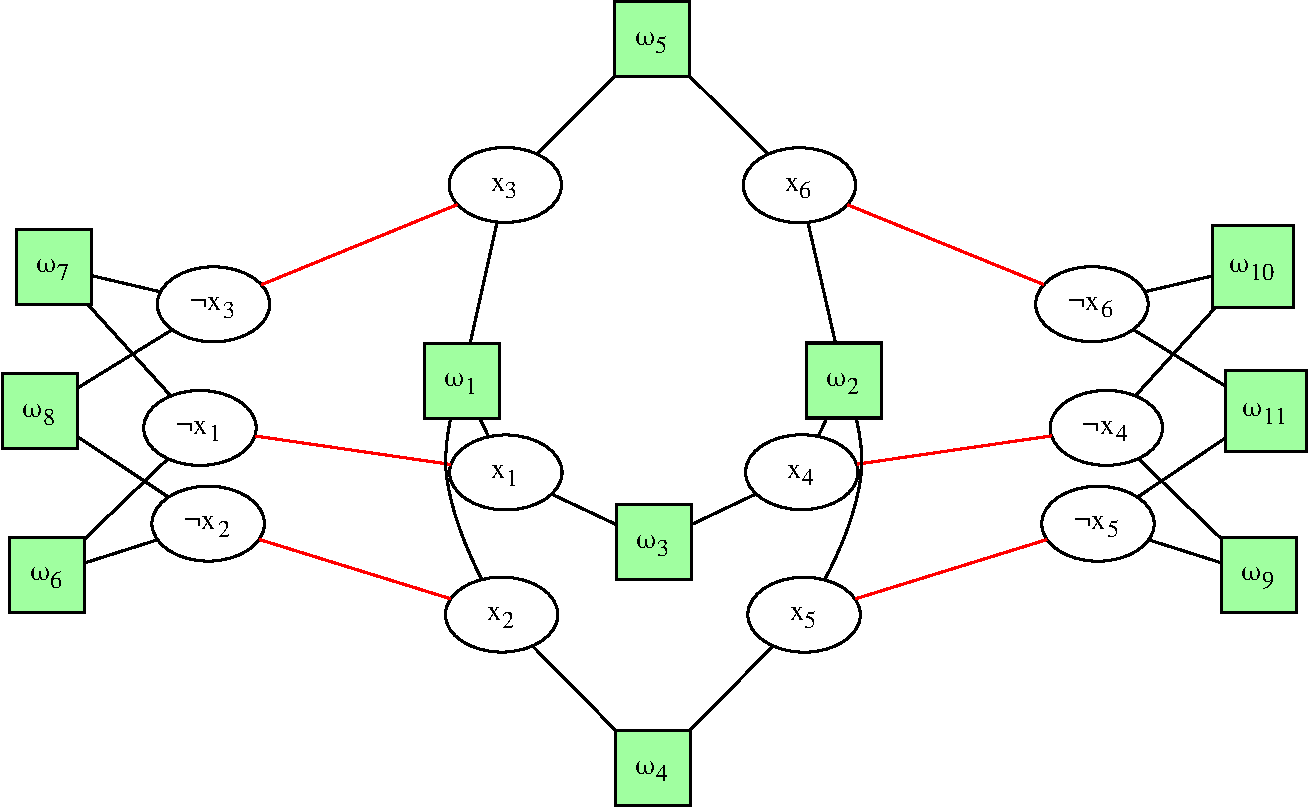
\includegraphics[width=4.3in]{cnfs/graph_cnf_no_opt-crop}
	\end{minipage}
\caption{Example of constructed symmetry graph for a given CNF}
\end{figure}

\hakan{Explication du graph + informations num nodes num edges. Probleme reel battleship
}

The battleship problems place one  ship of size *** and two ships of size* in grid 3x4 \\
1  2  3\\
4  5  6\\
7  8  9\\
10 11 12\\

one ship per row.\\

Produced graph contains 12 * 2 = 24  + 21 = 45 nodes and 24 + 36 = 60 edges 

\clearpage

An optimization of this graph is possible with the usage of binary clauses i.e. a clause with only two literals.
The clause node can be omitted and we connect the two literals. As we cannot distinguish between the optimized edge 
and boolean consistency edges, we must check if the produced permutations are spurious. 
To do so, as we ensure the permutation commutes with the negation it suffice to check:
$\forall x \in \support(g), g.\neg x = \neg g.x$.
Roughly speaking, we check if the image of the negation of $x$ is equals to the negation of the image of $x$, for each element $x$ in the support of the permutation.
This optimization allows to compute symmetries of the problem more efficiently.
In the previous example, the graph has deleted 12 nodes and 12 edges. More generally,
the graph removes as many nodes and edges as binary clauses on the formula.

\begin{figure}[h]
	\begin{minipage}[c]{.2\textwidth}
		\lstinputlisting[numbers=none]{cnfs/battleship-3-4-unsat.cnf}
	\end{minipage}
	\begin{minipage}[l]{.75\textwidth}
		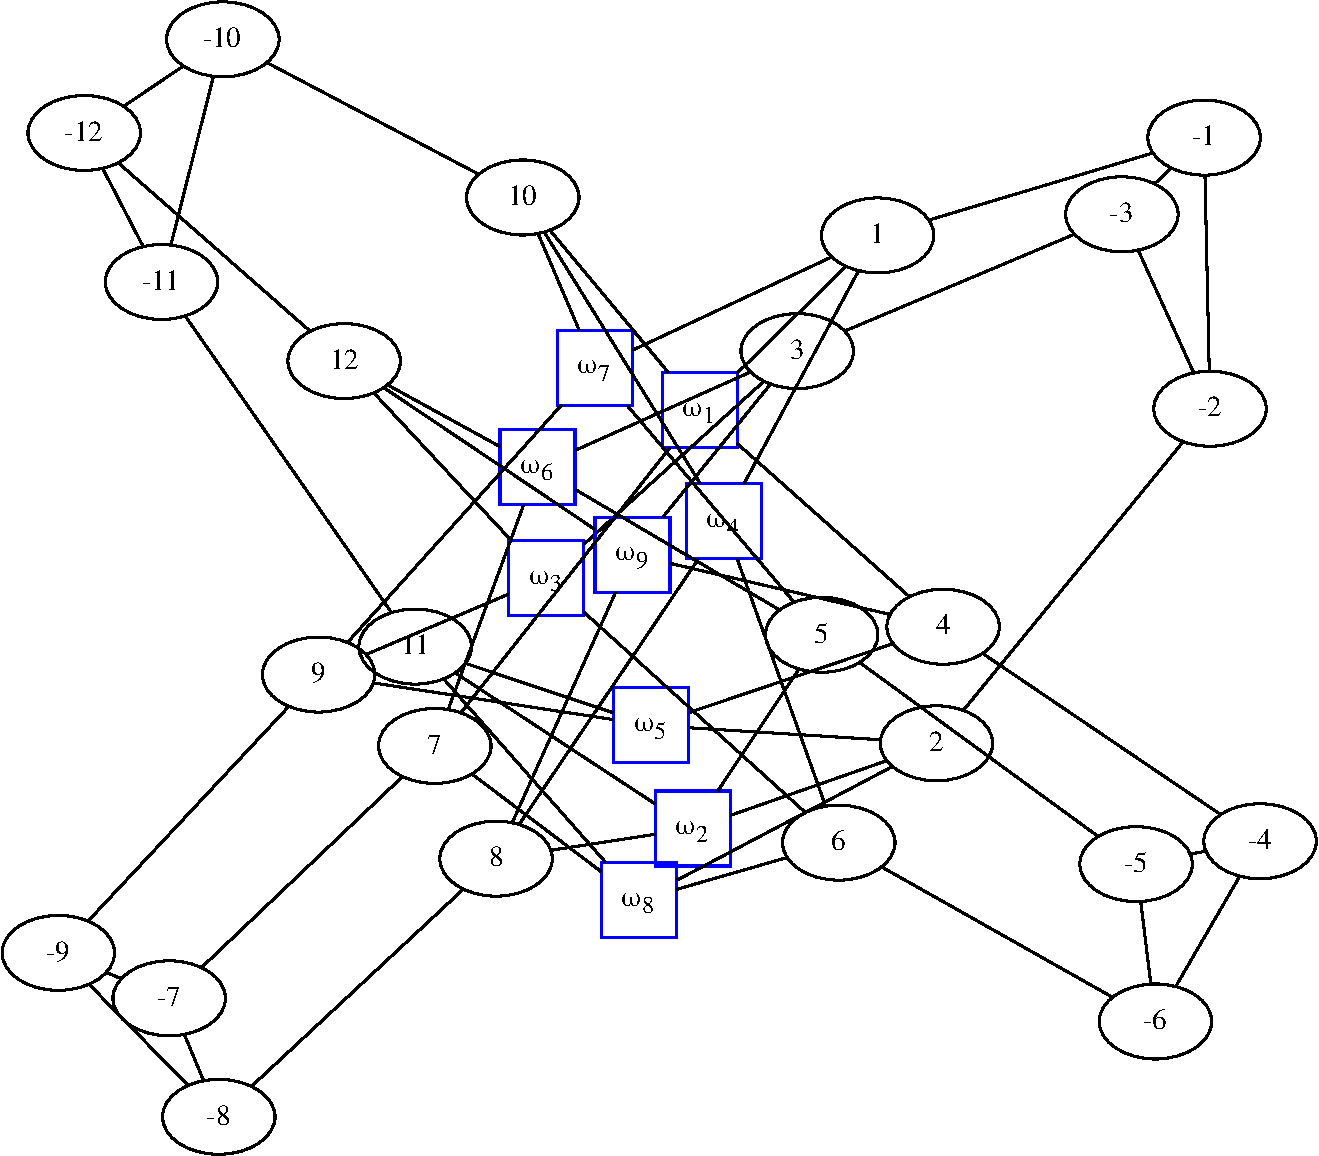
\includegraphics[width=4.3in]{cnfs/graph_cnf_opt-crop}
	\end{minipage}
	\caption{Example of constructed symmetry graph for a given CNF}
\end{figure}


%\hakan{optimisation du graph}\\
%\hakan{creation d'un probleme fil conducteur and utilisation de celui dans chaque partie, du calcul des symétries
%jusqu'au SBP}\\

When these graph is given to an automorphism tool like \bliss, the following \emph{generators} are 
obtained:
\begin{itemize}[topsep=0em]
\item $g_0$: (2 3)(5 6)(8 9)(11 12)(-2 -3)(-5 -6)(-8 -9)(-11 -12)
\item $g_1$: (4 5 6)(7 9 8)(-4 -5 -6)(-7 -9 -8)
\item $g_2$: (4 7)(5 8)(6 9)(-4 -7)(-5 -8)(-6 -9)
\item $g_3$: (1 2)(5 6)(7 9)(10 11)(-1 -2)(-5 -6)(-7 -9)(-10 -11)
\item $g_4$: (1 10)(2 11)(3 12)(-1 -10)(-2 -11)(-3 -12)
\end{itemize}


The visualization of the orbits of literals on the problem could be seen in figure~\ref{fig:orbits}, where each node represents a literal. Two literals are 
linked with an arc if it exists a permutation that maps the literal to the second one.
By definition of the orbits, each literal belongs to a strongly connected components (SCC).

 \begin{figure}[h]
 	\centering
 		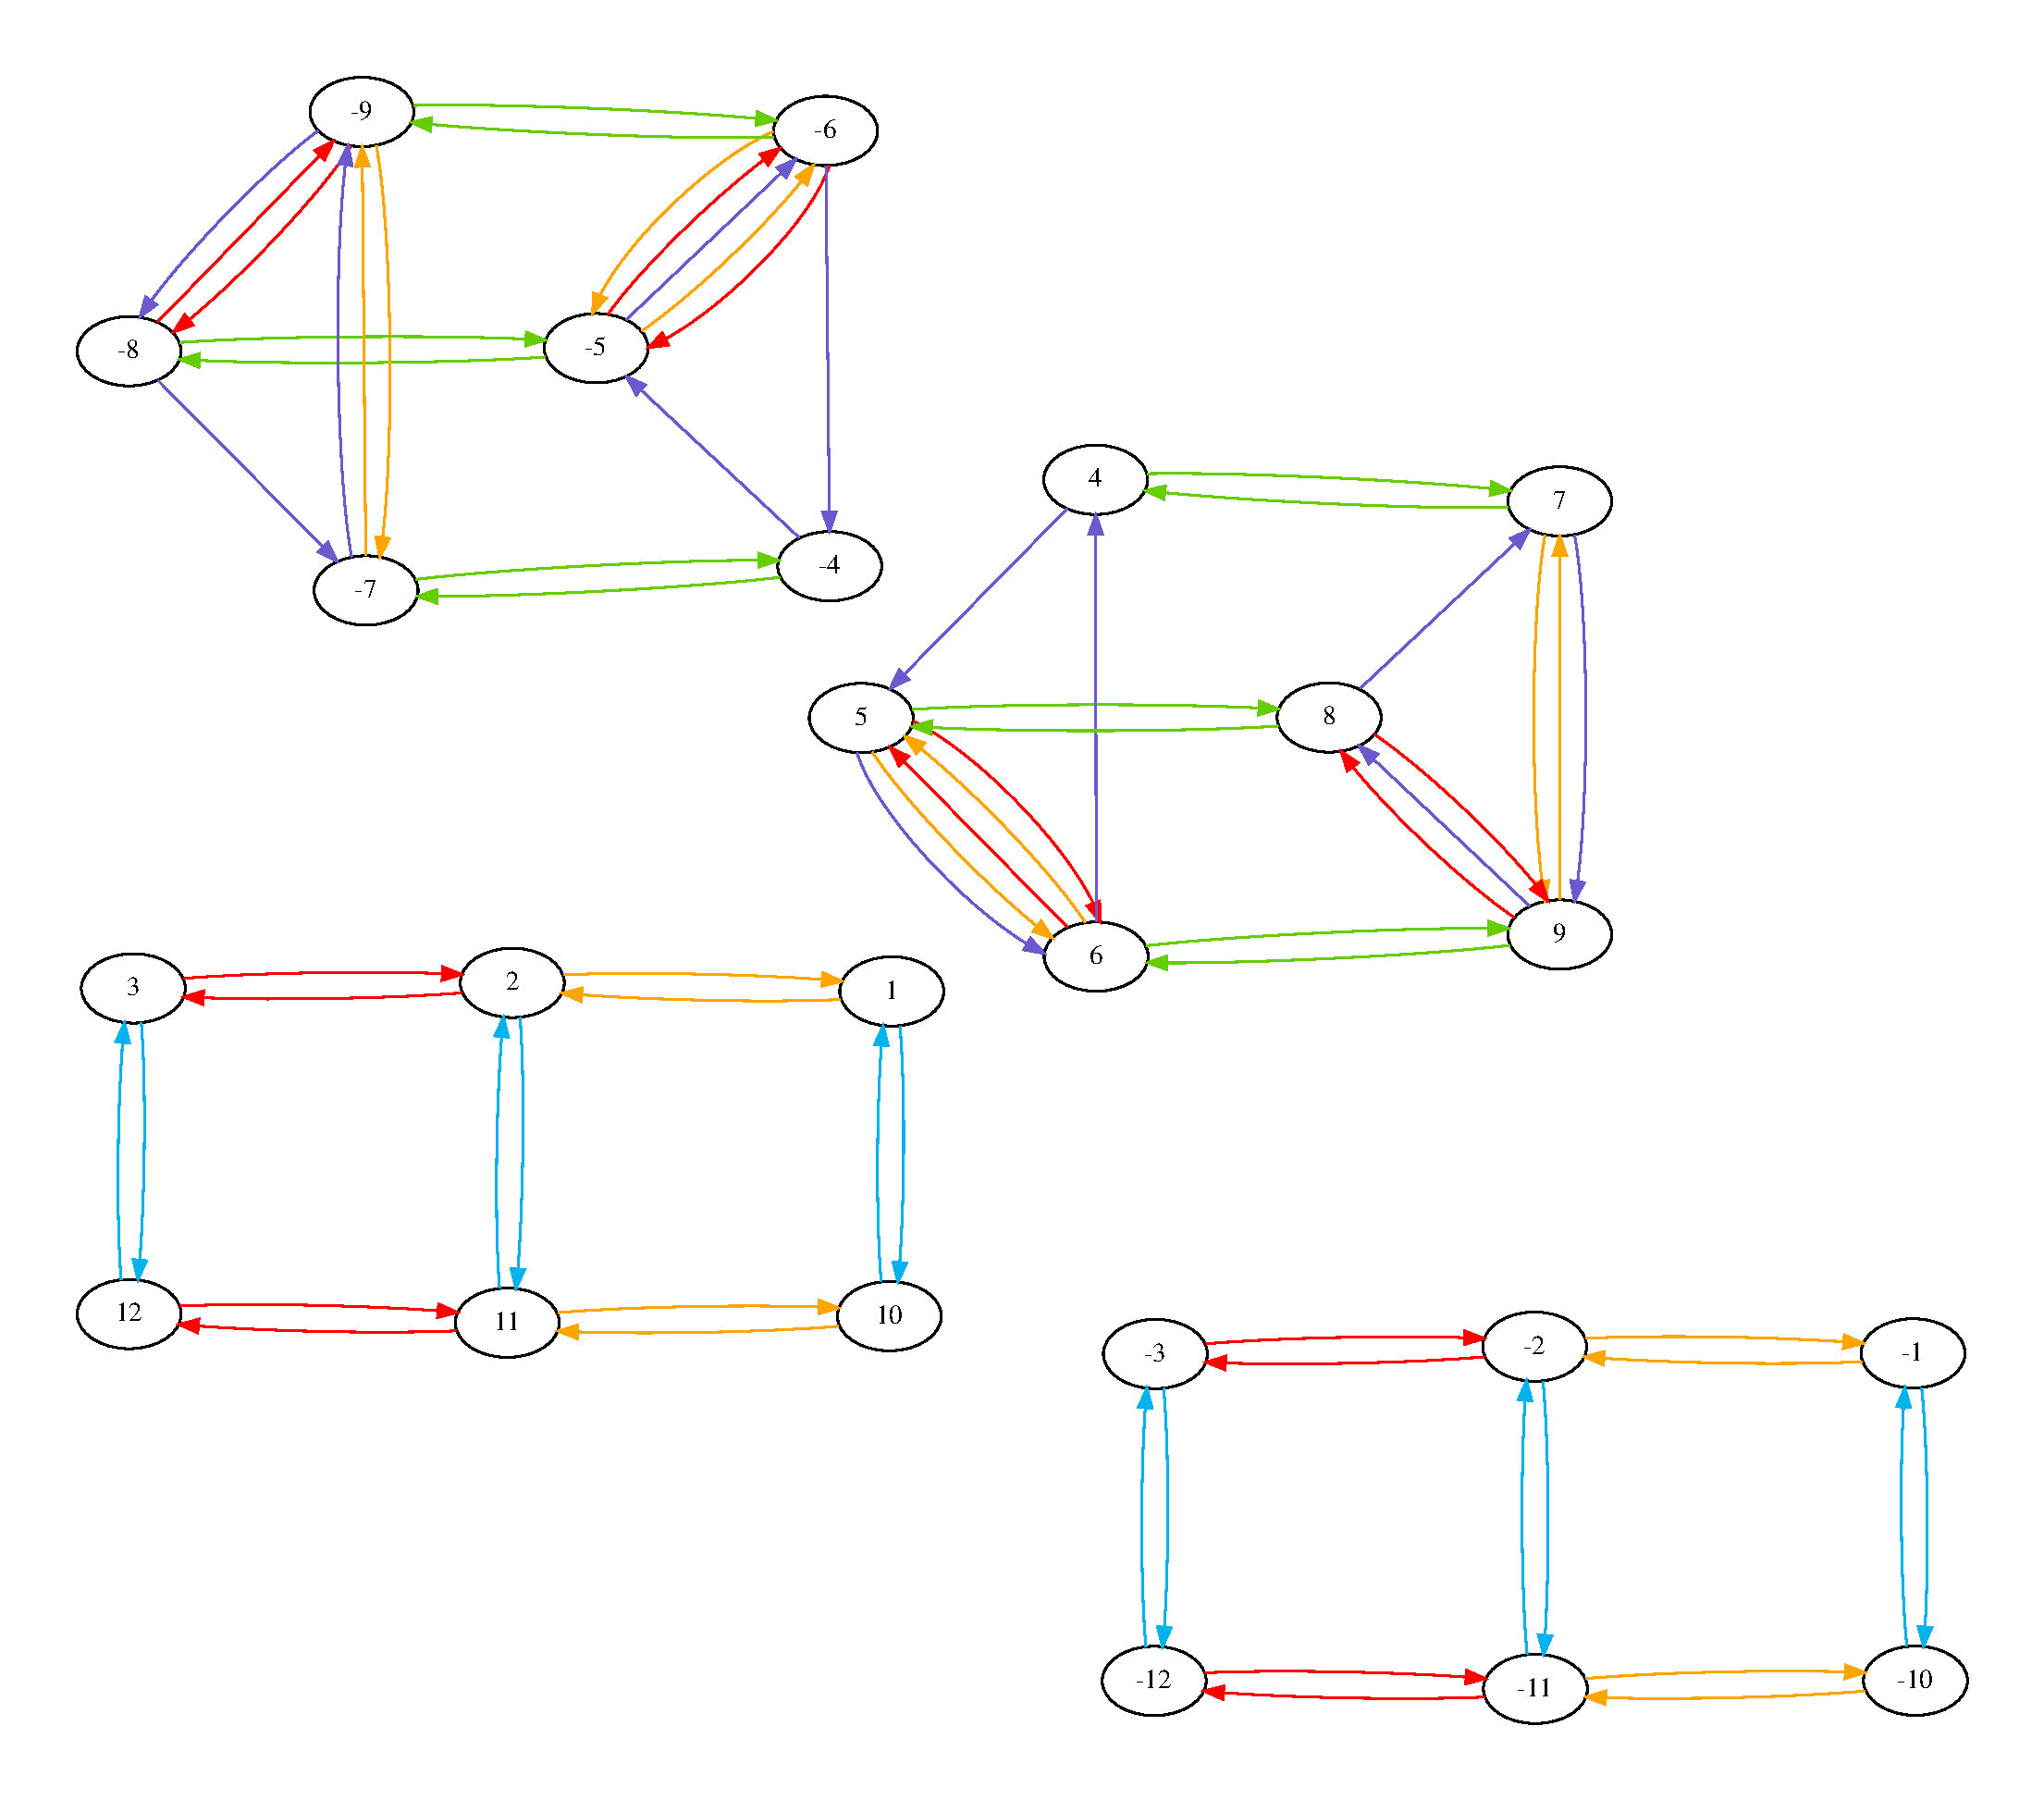
\includegraphics[width=\textwidth]{cnfs/orbits}
 	\caption{Orbits}
 	\label{fig:orbits}
 \end{figure}



\section{Usage of symmetries}

\emph{Symmetry breaking} aims at eliminating symmetry, either
by \emph{statically} posting symmetry breaking constraints that invalidate symmetric
assignments, or by altering the search space \emph{dynamically} to avoid symmetric search paths.


In order to exploit the symmetry properties of a SAT problem, we need to
introduce an ordering relation between the assignments.

\begin{definition}[Assignments ordering]
	\label{def:assignment_ordering}
	We assume a total order, $\prec$, on $\Vars$.  Given two assignments $(\alpha,\beta) \in \Assignments(\Vars)^2 $, 
	we say that $\alpha$ is strictly smaller than $\beta$, noted $\alpha < \beta$, if there exists a variable $v \in \Vars$
	such that:
	\begin{itemize}
		\item for all $v' \prec v$, either $v' \in \alpha \cap \beta$ or $\neg v' \in \alpha \cap
		\beta$.
		\item $\neg v \in \alpha$ and $v \in \beta$.\footnote{We could have chosen as well $v \in \alpha$ and $\neg v \in \beta$ without loss of generality.}
	\end{itemize}
\end{definition}

Note that $<$ coincides with the lexicographical order on \emph{complete}
assignments. Furthermore, the $<$ relation is monotonic as expressed in the following proposition:

\begin{proposition}[Monotonicity of assignments ordering]
	\label{prop:monocity_assignments_ordering}
	Let  $(\alpha,\alpha',\beta,\beta') \in \Assignments(\Vars)^4 $ be four assignments.
	$$\text{If}~\alpha \subseteq \alpha'~\text{and}~\beta \subseteq \beta',~\text{then}~\alpha < \beta \implies \alpha' < \beta'$$
\end{proposition}

\begin{proof}
	The proposition follows on directly from Definition \ref{def:assignment_ordering}.
\end{proof}


Let $\varphi$ a formula, and $G$ the group from the formula.
The \emph{orbit of $\alpha$ under $G$} (or
simply the \emph{orbit of $\alpha$} when $G$ is clear from the context) is the set
$ [\alpha]_G=\{ g.\alpha \mid g \in G \}$. The lexicographic leader
(\textit{lex-leader} for short) of an orbit $[\alpha]_G$ is defined by
$min_<([\alpha]_G)$. This \textit{lex-leader} is unique because the lexicographic
order is a total order.
The optimal approach to solve a symmetric SAT problem would be to explore
only one assignment per orbit (for instance each lex-leader). However, finding the
lex-leader of an orbit is computationally hard~\cite{Luks2004}. To avoid exploring 
symmetry search space, \emph{symmetry breaking predicates} are added to the formula.
These constraints are true only for the \emph{lex-leader} \cite{crawford1996symmetry}.




%\begin{definition}[Stabilizer of permutation]
%	Let two permutation $g_1$ and $g_2$, we say that $g_1$  stabilize $g_2$
%	$$\text{If}~ \support(g_1) \cap \support(g_2) = \emptyset$$
%\end{definition}


\begin{theorem}[Satisfiability preservation SBPs]
	\label{theorem:satisfiability_preservation_SBPs}
	Let $\varphi$ be a formula and $\psi$ the computed \textit{SBPs} for the set of
	symmetries $S(\varphi)$
	
	$$\varphi~and ~\varphi \wedge \psi \text{ are equi-satisfiable}.$$
\end{theorem}

\begin{proof}
	If $\varphi \wedge \psi$ is SAT then $\varphi$ is trivially SAT. If
	$\varphi$ is SAT, then there is some assignment $\beta$ that satisfies $\varphi$.
	Without loss of generality, $\beta$ can be chosen to be the lex-leader of its
	orbit under $S(\varphi)$. Thus, $g$ does not contradict $\beta$, which implies that
	$\beta \models \psi$.
\end{proof}

 
\hakan{Refaire la figure avec plus de point}
\begin{figure}
	\centering
%	\includegraphics[width=2in]{fig/assignment-lex-leader}
	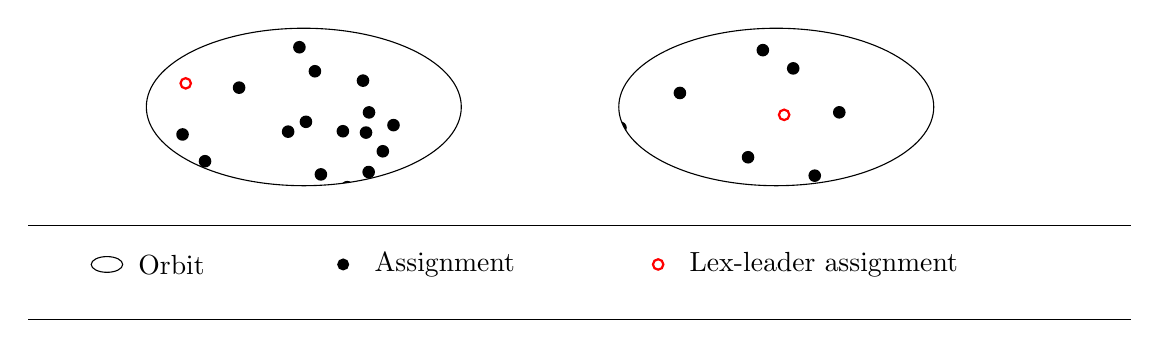
\begin{tikzpicture}
    \tikzstyle{point}=[circle,draw,thick,fill=black,scale=0.2]
	\tikzstyle{point+}=[circle,draw=red,thick,scale=0.4]


\begin{scope}
\node[ellipse, draw, minimum width=4cm, minimum height=2cm] (c1) at (2.5,0){};
	\clip (2.5, 0) ellipse (2 and 1);
	\node[point+] (p2) at (1, 0.3){};
	\pgfmathsetseed{281}
	\foreach \p in {1,...,100}
	{
		\fill (4*rand,2*rand+0.25) circle (0.08);
	}
\end{scope}


\begin{scope}
\node[ellipse, draw, minimum width=4cm, minimum height=2cm] (c1) at (8.5,0){};
\clip (8.5,0) ellipse (2 and 1);
\node[point+] (p2) at (8.6, -0.1){};
\pgfmathsetseed{499478626}
\foreach \p in {1,...,40}
{
	\fill (4*rand+6,2*rand) circle (0.08);
}
\end{scope}

% Legend

\path[draw] (-1, -1.5) -- (13, -1.5);
\node[draw,ellipse, draw, minimum width=4cm, minimum height=2cm, scale=0.1] (ld) at (0, -2) {};
\node[align=left, text width=2.2cm] at (1.5, -2) {Orbit};


\node[circle, fill=black, draw=black, line width=0.5mm, scale=0.3] (lz) at (3, -2) {};
\node[align=left, text width=2.2cm] at (4.5, -2) {Assignment};


\node[point+] (le) at (7, -2) {};
\node[align=left, text width=4.2cm] at (9.5, -2) {Lex-leader assignment};

\path[draw] (-1, -2.7) -- (13, -2.7);



\end{tikzpicture}
	\caption{One lex-leader per assignment}
\end{figure}


It exists two kind of symmetry breaking, the first one is \emph{full symmetry breaking} and it 
aims to visit exactly one assignment per orbit (generally the lex-leader). This
approach is in practice infeasible in the most case due to the exponential number of permutations in a group.
The second one is \emph{partial symmetry breaking} and it aims to visit at least one assignment per orbit. This approach is easy to set up and bring us to considerable reduction of the search spaces. The used set
of permutations is generally the set of generators of a formula given by the automorphism tool.

An extremely important point is the chosen lexicographic order.
Variable ordering may impact the number of generated constraint and so the performance of
the underlying SAT solver. Different orders are studied in the literature. 
One of the simplest order was the sorted variables according to their numbers.
Some others orders exists and exploit structural properties of the 
problem. In particular, the orbits of the variables in different ways. For example, the variables are chosen 
with their number of occurrences in the initial problem. This order, is equivalent to put largest orbit first
and so on, because each variable on the same orbit must have the same number of occurrences.
Another example of exploiting structural property of the orbit is the usage of \emph{stabilizer}.
The order choose a variable which maximize the number of stabilized permutations, removes the not stabilized ones and loop over until the empty set. The remaining variables are added to the order to get a complete order.




\subsection{Static symmetry breaking}
The exploitation of symmetries statically is called \emph{static symmetry breaking}.
It acts like a preprocessor which add \emph{symmetry breaking predicates} (SBPs) at the 
original formula and solve the augmented problem. 
This approach gives good performances in practice.

\hakan{Generation des clauses de SBPs}\\
\hakan{Parler des groupes speciaux  (totaux) }\\
\hakan{Generation des clause binaires breakid lie aux orbits}\\
\hakan{Parler de BreakID all in one tout au dessus}\\

\hakan{Put a complete exemple}\\

\hakan{Mettre des courbes}\\
\hakan{Tableau sur le nombre de sbp genere}\\


\hakan{Conclu static}

In the general case,
the size of the \textit{sbp} can be exponential in the number of variables of
the problem so that they cannot be totally computed. The underlying SAT solver can 
 Even in more favorable
situations, the size of the generated \textit{sbp} is often too large to be
effectively handled by a SAT solver~\cite{Luks2004}. On the other hand, if
only a subset of the symmetries is considered then the resulting search pruning
will not be that interesting and its effectiveness depends heavily on the
heuristically chosen symmetries \cite{biere2009handbook}.



\hakan{Drawbacks de la methode pourquoi on fait du dynamique}

\subsection{Dynamic symmetry breaking}


Another disadvantage is that the solver is influenced by SBPs and explore the search space with a different 
manner and can affect performance negatively \hakan{FIND A REF}

A different approach can be used to reduce search space using symmetries is \emph{symmetry propagation}~\cite{Devriendt12}.
The general idea of this approach is to propagate symmetrical literals of already propagated literals.
In other words, it tries to accelerate the tree traversal by ``transforming some guessing to deductions''.
Indeed, knowing that the processed problem presents symmetries makes it possible to deduce some values 
for the variables that would be guessed if those symmetries were ignored.
These deductions will reduce the overall tree traversal depth and hence eventually accelerate the solving process.


\hakan{Mettre logical conqequence quand on explique CDCL + Expliquer CDCL plus en detail avec les learnt et les raisons}

\begin{definition}[Logical consequence]
	\label{def:logical_consequence}
	A formula $\phi$ is a logical consequence of a formula $\varphi$ denoted by $\varphi \models \phi$ if for all assignment
	$\alpha$ satisfying $\varphi$, it satisfies also $\phi$. Two formulas are \emph{logically equivalent} if each is a logical
	consequence of the other.
\end{definition}


\begin{proposition}[Symmetry propagation]
	\label{prop:symmetry_propagation}
	Let $\varphi$ be a formula, $\alpha$ an assignment and $l$ a literal. 
	If $g$ is a symmetry (permutation) of $\varphi \cup \alpha$ and
	$\varphi  \cup \models \{l\}$, then $\varphi \cup \alpha \models g.\{l\}$ is also true.
\end{proposition}

In other words, if a literal $l$ was propagated by the solver and $g$ is a \emph{valid} symmetry for the
sub problem $\varphi \cup \alpha$ (in which all satisfied clauses and literals are removed), so , the solver can
also propagate the symmetrical of $l$. The problem here is to determinate which symmetries are valid for the formula
$\varphi \cup \alpha$.

\begin{definition}[Active symmetry]
	A symmetry $g$ is called active under a partial assignment $\alpha$ $\text{if } g.\alpha = \alpha$
\end{definition}

Which leads to the following proposition

\begin{proposition}
	\label{prop:active_symmetry}
	Let $\varphi$ a formula and $\alpha$ a partial assignment. Let $g$ a symmetry of $\varphi$,
	if $g$ is active under the assignment $\alpha$, then $g$ is also a symmetry of $\varphi \cup \alpha$
\end{proposition}

The previous proposition states that an active symmetry $g$ for a partial assignment $\alpha$ still valid for
the formula $\varphi \cup \alpha$. So when a literal $l$ is propagated, and a symmetry $g$ is active for a
partial assignment $\alpha$, the solver can also propagate $g.l$. Moreover, with the group theory, permutations can be
composed, the composition of two active symmetries is also an active symmetries and can propagate $g^2.l, g^3.l, ... $

\hakan{Peut etre expliquer les sym conflicts}


The authors of symmetry propagation improve the active symmetries, introducing \emph{weakly active} symmetries.

\begin{definition}[Weakly active symmetry]
	\label{def:weakly_active_symmetry}
	Let $\varphi$ a formula and ($\delta, \alpha, \gamma$) a state of a CDCL solver in which $\delta$ is the set of decisions,
	$\alpha$ is the current assignment and $\gamma$ the reasons of the learned clauses. Then a symmetry $g$ is weakly active 
	if $g.\delta \subseteq \alpha$
\end{definition}

This definition leads to the following proposition:

\begin{proposition}
	Let $\varphi$ be a formula, $\alpha $ an assignment. If
	there exists a subset $\delta \subseteq \alpha $ and a symmetry $g$ of $\varphi$ such that 
	$g.\delta \subseteq \alpha $ and $\varphi \cup \delta \models \varphi \cup \alpha$, then $g$ 
	is also a symmetry of $\varphi \cup \alpha $.
\end{proposition}

\hakan{Proof}



\hakan{Detail SP}\\
\hakan{Logical consequence of a formula }\\
\hakan{Symmetry active}\\
\hakan{Symmetry weakly active}\\
\hakan{Courbe VS static an no sbp}\\
\hakan{Conclu SP, depend on the solver choice }


\hakan{Detail Symmetry Explanation Learning (SEL), apprendre les symmetriques des clauses}


%\begin{proposition}[Satisfiability preservation]
%	\label{prop:equi_satisfiability}
%	 Let $\varphi$ a CNF problem and $\psi$ the computed symmetry breaking predicates.
%	 Solve $\varphi \cup \psi$ is equi-satisfiable to solve $\varphi$.
%\end{proposition}
%
%\begin{proof}
%	On the first case, if the initial formula $\varphi$ is \unsat,
%	then the augmented problem $\varphi \cup \psi$ is trivially \unsat.
%	On the second case, if $\varphi$ is \sat then $\varphi \cup \psi$ is also \sat because 
%	$\psi$ forbids only non lex-leader assignment so the formula still be \sat.
%\end{proof}



%% Local Variables:
%% TeX-master: "main.tex"
%% ispell-dictionary: "en_US"
%% mode: latex
%% mode: flyspell
%% coding: utf-8
%% End:


\part{Contributions}
\setcounter{mtc}{4} 
\chapter{SymmSAT: Between Static and Dynamic\\ Symmetry Breaking}\label{chap:symmSAT}
\minitoc
This chapter presents our first contribution published in TACAS 2018 conference~\ref{algorithm:cdcl_cosy}. 
\section{General idea}
%\subsubsection{Drawbacks of the static-based approaches.} 
In the static symmetry breaking approach constraints are added to the original 
problem that avoids the solver to visit symmetrical search space.
But, in the general case,
the size of the \textit{sbp} can be exponential in the number of variables of
the problem so that they cannot be entirely computed. Even in more favorable
situations, the size of the generated \textit{sbp} is often too large to be
effectively handled by a SAT solver~\cite{Luks2004}. On the other hand, if
only a subset of the symmetries is considered then the resulting search pruning
will not be that interesting and its effectiveness depends heavily on the
heuristically chosen symmetries \cite{biere2009handbook}. Besides, these approaches
are preprocessors, so their combination with other techniques, such as
\emph{symmetry propagation}~\cite{Devriendt12}, can be very hard. Also, tuning
their parameters during  solving time turns out to be tough. For all
these reasons, some classes of SAT problems cannot be solved easily yet despite
the presence of symmetries.
To handle these issues, we propose a new
approach that reuses the principles of the static approaches, but operates
dynamically: the symmetries are broken during the search process without any
pre-generation of the \textit{sbp}. It is a best effort approach that tries to eliminate,
\textit{dynamically}, the \textit{non lex-leading} assignments with a minimal
computation effort. To do so, we first introduce the notions of
\textit{reducer}, \textit{inactive} and \textit{active} permutations (with
respect to an assignment $\alpha$) and \emph{effective symmetric breaking predicates} (\emph{esbp}).
\begin{definition}[Reducer, inactive and active permutation]
  A permutation $g$ is a \emph{reducer} of an assignment $\alpha$ if $g.\alpha < \alpha$ 
  (hence $\alpha$ cannot be the lex-leader of its orbit. The permutation  $g$ reduces the assignment and all its extensions).\\
 The permutation $g$ is \emph{inactive} on $\alpha$ when $\alpha < g.\alpha$ (so $g$ cannot reduce $\alpha$ and all
 its extensions). A symmetry is said to be \emph{active} with respect to $\alpha$
 when it is neither inactive nor a reducer of $\alpha$. 
\end{definition}
Proposition~\ref{prop:status} restates this definition in terms of variables
and is the basis of an efficient algorithm to track the status of a
permutation during the solving. Let us, first, recall that the \emph{support}
 of a permutation $g$, $\support_g$, is the set $\{ v \in \Vars \mid g.v \neq v\}$.
 \clearpage 
\begin{proposition}
 \label{prop:status}
 Let $\alpha \in \Assignments(\Vars)$ be an assignment, $g \in \Group$, a permutation and $ \support_g \subseteq  \Vars$ the support of $g$. We say that $g$ is:
 \begin{enumerate}
  \item  \emph{a reducer of} $\alpha$  if there exists a variable $v \in \support_g$
  such that:
  \begin{itemize}
   \item $\forall\ v' \in \support_g$, s. t. $v' \prec v$, either $\{v', g^{-1}(v')\}\subseteq\alpha $ or $\{\neg v', \neg g^{-1}(v')\} \subseteq \alpha $,
   \item $\{v, \neg g^{-1}(v)\} \subseteq \alpha$;
  \end{itemize}
  \item  \emph{inactive} on $\alpha$  if there exists a variable $v \in \support_g$
  such that:
  \begin{itemize}
   \item $\forall\ v' \in \support_g$, s. t. $v' \prec v$, either $\{v', g^{-1}(v')\}\subseteq\alpha $ or $\{\neg v', \neg g^{-1}(v')\} \subseteq \alpha $,
   \item $\{\neg v, g^{-1}(v)\} \subseteq \alpha$;
  \end{itemize}
  \item  \emph{active} on $\alpha$, otherwise.
 \end{enumerate}
\end{proposition}


When $g$ is a \textit{reducer} of $\alpha$ we can define a predicate that contradicts $\alpha$ and yet preserves the satisfiability of the formula. Such a predicate will be used to discard $\alpha$, and all its extensions, from a further visit and hence prune the search tree.
\begin{definition}[Effective Symmetry Breaking Predicate]
 \label{def:esbp}
 Let $\alpha \in \Assignments(\Vars)$, and $g \in \Group_{\Vars}$.
 We say that the formula $\psi$ is an effective symmetry breaking predicate (\textit{esbp} for short) for $\alpha$ under $g$ if:
 $$\alpha \not\models \psi \text{ and for all }\beta \in \Assignments(\Vars), \beta \not\models \psi \Rightarrow g.\beta < \beta$$
\end{definition}
The next definition gives a way to obtain such an effective symmetry-breaking predicate from an assignment and a reducer.
\begin{definition}[A construction of an \emph{esbp}]\label{def:eta}
 Let $\varphi$ be a formula.
 Let $g$ be a symmetry of $\varphi$ that reduces an assignment $\alpha$.
 Let $v$ be the variable whose existence is given by item 1. in Proposition~\ref{prop:status}.
 Let $U = \{ v', \neg v' \mid v' \in \Vars_g \text{ and } v'~\preceq~v\}$.
 We define $\eta(\alpha, g)$ as $(U \cup g.U) \setminus \alpha$.
\end{definition}

\textbf{Example}. Let us consider $\Vars = \{x_1, x_2, x_3, x_4, x_5\}$, $g =
(x_1\,x_3)(x_2\,x_4)$, and a partial assignment $\alpha = \{x_1, x_2,
x_3, \neg x_4\}$. Then, $g.\alpha = \{x_1, \neg x_2, x_3, x_4\}$ and $v = x_2$.
So, $U = \{x_1, \neg x_1, x_2, \neg x_2\}$ and $g^{-1}.U = \{x_3, \neg x_3,
x_4, \neg x_4\}$ and following the Definition \ref{def:eta}, we can deduce than $\eta(\alpha, g) = (U \cup g.U)
\setminus \alpha = \{\neg x_1, \neg x_2, \neg x_3, x_4\}$.
\begin{proposition}
 \label{prop:eta}
 $\eta(\alpha, g)$ is an effective symmetry-breaking predicate.
\end{proposition}
\begin{proof}
 It is immediate that $\alpha \not\models \eta(\alpha, g)$.
 
 Let $\beta \in \Assignments(\Vars)$ such that $\beta \wedge \eta(\alpha, g)$ is \unsat. We denote a $\alpha'$
 and $\beta'$ as the restrictions of $\alpha$ and $\beta$ to the variables in $\{ v' \in
 \Vars_g \mid v'~\preceq~v \}$. Since $\beta \wedge \eta(\alpha, g)$ is \unsat, $\alpha' = \beta'$.
 But $g.\alpha' < \alpha'$, and $g.\beta' < \beta'$. By monotonicity of $<$, we thus also have
 $g.\beta < \beta$. \end{proof}
\medskip\noindent It is important to observe that the notion of \textit{ebsp}
is a refinement of the classical concept of \textit{sbp} defined in \cite{aloul06}. Specifically, like \textit{sbp}, \textit{esbp} preserve satisfiability.

\begin{theorem}[Satisfiability preservation]
 Let $\varphi$ be a formula and $\psi$ an \textit{esbp} for some assignment $\alpha$ under $g \in G_{\varphi}$. Then,
 $$\varphi~and ~\varphi \wedge \psi \text{ are equi-satisfiable}.$$
\end{theorem}
\begin{proof}
 
 If $\varphi \wedge \psi$ is SAT then $\varphi$ is trivially SAT. If
 $\varphi$ is SAT, then there is some assignment $\beta$ that satisfies $\varphi$.
 Without loss of generality, $\beta$ can be chosen to be the lex-leader of its
 orbit under $G_{\varphi}$. Thus, $g$ does not reduce $\beta$, which implies that
 $\beta \models \psi$.
 
\end{proof}

\subsection{Algorithm}
This section describes how to augment the state-of-the-art CDCL algorithm with
the aforementioned concepts to develop an efficient symmetry-guided SAT
solving algorithm. 
The approach is implemented using a couple of components: (1) a
\textit{Conflict Driven Clauses Learning (CDCL) search engine}; (2) \textit{a symmetry controller}. Roughly speaking, the first component performs the
classical search activity on the SAT problem, while the second observes the
engine and maintains the status of the symmetries. When the controller detects
a situation where the engine is starting to explore a redundant
part\footnote{Isomorphic to a part that has been/will be explored.}, it orders
the engine to operate a backjump. The detection is performed thanks to
\emph{symmetry status tracking} and the backjump order is given by a simple
injection of an \emph{esbp} computed on the fly.
%Principle of CDCL is described in section \ref{sec:cdcl}, 
\Cref{algorithm:cdcl_cosy} explains how to extend the CDCL algorithm described in \Cref{sec:cdcl}  with a \emph{symmetry controller} component.% which guides the behavior of CDCL algorithm depending on the status of symmetries.
\begin{algorithm}[!htbp]
	\SetKwProg{Fn}{function}{}{}
	\SetKwData{C}{SymController}
	\SetKwFunction{CDCL}{CDCLSym}
	\SetKwFunction{unitPropagation}{unitPropagation}
	\SetKwFunction{analyzeConflict}{analyzeConflict}
	\SetKwFunction{addLearntClause}{addLearntClause}
	\SetKwFunction{assignNewLiteral}{assignDecisionLiteral}
	\SetKwFunction{backjumpPolicy}{backjumpAndRestartPolicies}
	\SetKwFunction{isNotMinimal}{isNotLexLeader}
	\SetKwFunction{SBP}{generateEsbp}
	\SetKwFunction{notifyAssigned}{updateAssign}
	\SetKwFunction{notifyCancelled}{updateCancel}
	\SetKwFunction{symmetryController}{symmetryController}

	\DontPrintSemicolon
	
	\Fn{\CDCL{$\varphi$: CNF formula, {\color{red}\C: symmetry controller}}
		\textbf{returns} $\true$ if $\varphi$ is \sat and $\false$ otherwise}
	{
		$dl \gets 0$ \tcp*{Current decision level}
		$\alpha \gets \emptyset$\;
		\While {not all variables are assigned} {
			$isConflict \gets$ \unitPropagation{}\;
			{
				\color{red} 
				\C.\notifyAssigned{$\alpha$}\;\label{algo:cdcl_sym:notify}
				$isReduced \gets$ \C.\isNotMinimal{$\alpha$}\;\label{algo:cdcl_sym:not_minimal}
			}
			
			\If{$isConflict \, {\color{red}||\, isReduced}$} {
				\If{dl == 0}
				{
					\Return \false
					\tcp*{$\varphi$ is $\unsat$}
				}
				\If{\color{red}$isConflict$}
				{
					$\omega \gets$ \analyzeConflict{}\;
				}
				\Else {
					{
						\color{red}$\omega \gets$ \C.\SBP{$\alpha$}\;\label{algo:cdcl_sym:gen_esbp}
					}
				}
			$\varphi \gets \varphi \cup \{\omega$\} \;
				$dl \gets$ \backjumpPolicy{}\;
				{\color{red}\C.\notifyCancelled{$\alpha$}\;} \label{algo:cdcl_sym:cancel}
			}
			\Else{
				$\alpha \gets \alpha\, \cup $ \assignNewLiteral{}\; 
			$dl \gets dl+1$\;
			}
		}
		\Return \true
		\tcp*{$\varphi$ is $\sat$}
		
	}
	\caption{the CDCLSym SAT Solving Algorithm.}
	\label{algorithm:cdcl_cosy}
\end{algorithm}


 
 The symmetry controller is initially given a set of symmetries $G$, the generators of the group of symmetries. It observes the behavior of the SAT engine and updates its internal data according to the current assignment, to keep track of the status of the symmetries. This observation is \emph{incremental}: whenever a literal is assigned or canceled, the symmetry controller updates the status of all the symmetries. This corresponds to \cref{algo:cdcl_sym:notify,algo:cdcl_sym:cancel} of Algorithm~\ref{algorithm:cdcl_cosy}. When the controller detects that the
 current assignment cannot be a \emph{lex-leader} (\cref{algo:cdcl_sym:not_minimal}), it generates the
 corresponding \emph{esbp} (\cref{algo:cdcl_sym:gen_esbp}).
 
 \medskip\noindent In the remainder of this section, functions
 composing the symmetry controller are detailed.
 
 \subsubsection{Symmetries Status Tracking.} The \texttt{updateAssign},
 \texttt{updateCancel} and \texttt{isNot\-LexLeader} functions (\Cref{algo:keep_status}) track the status of symmetries based on
 Proposition~\ref{prop:status} ; there resides the core of our algorithm.
 
 All these functions rely on the $\track$ structure: a map of variables indexed
 by permutations. Initially, $\track[g] = \min_{\prec}(\support_g)$ for all $g \in G$ according to the ordering relation and all
 permutations are marked \textit{active}. 
 
 For each permutation $g$, the symmetry controller keeps track of the smallest
 variable $\track[g]$ in the support of $g$ such that $\track[g]$ and
 $g^{-1}(\track[g])$ do not have the same value in the current assignment. If
 one of the two variables is not assigned, they are considered  to have different values.
 
 When new literals are assigned, only active symmetries need to have their
 $\track[g]$ updated (\cref{alg:esbp:update}). This update is done thanks to a while
 loop (\cref{alg:esbp:loop1,alg:esbp:loop2}).
 
 When literals are canceled, we need to update the status of symmetries for
 which some variable $v$ before $\track[g]$, or $g^{-1}(v)$, becomes unassigned
 (\cref{alg:esbp:min}). Symmetries that were inactive may be reactivated (\cref{alg:esbp:reactivate}).
 
 The current assignment is not a \textit{lex-leader} if some symmetry $g$ is a
 reducer. This is detected by comparing the value of $\track[g]$ with the value
 of $g^{-1}(\track[g])$ (\cref{alg:esbp:notmin}). The function \texttt{isNotLexLeader} also
 marks symmetries as \emph{inactive} when appropriate (\cref{alg:esbp:inactive1,alg:esbp:inactive2}).
 
 \subsubsection{Generation of the \emph{esbp}.} When the current assignment
 cannot be a \textit{lex-leader}, some symmetry $g$ is a reducer. The function
 \texttt{generateEsbp} computes the $\eta(\alpha, g)$ of Definition~\ref{def:eta},
the effective symmetry-breaking predicate of Proposition~\ref{prop:eta}. This will
 prevent the CDCL engine to explore further the current partial assignment.
 
 \begin{algorithm}[!htbp]
 \SetKwProg{Fn}{function}{}{}
  \SetKwFunction{notifyAssigned}{updateAssign}
  
  \Fn{\notifyAssigned{$\alpha$: assignment}
  }{
   \ForEach{active $g \in  G$}{\label{alg:esbp:update}
    $v \gets \track[g]$\;
    \While{ $\{v, g^{-1}(v)\}\subseteq\alpha $ \textbf{or} $\{\neg v, \neg g^{-1}(v)\} \subseteq\alpha$ }{ \label{alg:esbp:loop1}
     $v \gets$ next variable in $\Vars_g$\; \label{alg:esbp:loop2}
    }
    $\track[g] \gets v$
   }
  }
  
  \Fn{\notifyCancelled{$\alpha$: assignment}}{
   \ForEach{$g \in G$}{
    $u \gets \min \{ v \in \Vars_g \mid \{v, \neg v\} \cap \alpha = \emptyset \text{ or } \{g^{-1}(v), \neg g^{-1}(v)\} \cap \alpha = \emptyset \}$\;\label{alg:esbp:min}
    \If{$u \preceq \track[g]$}{
     mark $g$ as active\;\label{alg:esbp:reactivate}
     $\track[g] \gets u$\;
    }
    
   }
  }
  
  \Fn{\isNotMinimal{$\alpha$: assignment}}{
   \ForEach{active $g \in G$}{
    $v \gets \track[g]$\;
    \If{$\{v, \neg g^{-1}(v)\}\subseteq\alpha$} {\label{alg:esbp:notmin}
     \Return \true  \tcp*{$g$ is a reducer}
    }
    \If{$\{\neg v, g^{-1}(v)\}\subseteq\alpha$}{\label{alg:esbp:inactive1}
     mark $g$ as inactive \label{alg:esbp:inactive2}
     \tcp*{$g$ can't reduce $\alpha$ or its extensions}
    }
    
   }
   \Return \false
  }
  
  
  \Fn{\SBP{$\alpha$: assignment} \textbf{returns} $\omega$: generated $esbp$}
  {
   $\omega \gets \{\}$\;
   $g \gets$ the reducer of $\alpha$ detected in \isNotMinimal\;
   $v \gets min(\Vars_g)$\;
   $u \gets \track[g] $\;
   \While{$u \neq v$}{
    \leIf{$v \in \alpha$} {$\omega \gets \omega \cup \{\neg v\}$}{$\omega \gets \omega \cup \{v\}$}
    \leIf{$g^{-1}(v) \in \alpha$} {$\omega \gets \omega \cup \{\neg g^{-1}(v)\}$}{$\omega \gets \omega \cup \{g^{-1}(v)\}$}
    $v \gets$ next variable in $\Vars_g$
   }
   $\omega \gets \omega \cup \{\neg v, g^{-1}(v)\}$\;
   \Return $\omega$
  }
  \caption{the functions keeping track of the status of the symmetries and generating the \emph{esbp}.}
  \label{algo:keep_status}
  
 \end{algorithm}%
 
 
 
 \subsection{Illustrative example}
  Let us illustrate the previous concepts and algorithms on a simple example. Let the ordering relation be $x_1 \prec x_2 \prec x_3 \prec x_4
 \prec x_5 \prec x_6\ \mid \false < \true$, and two generators:\\
 $G = \{
  g_1 = (x_1 \enskip x_2)(x_4 \enskip x_5),g_2 = (x_1 \enskip x_4)(x_2 \enskip x_5)(x_3 \enskip x_6)\}$
 (written in cycle notation with opposite cycles omitted). Their
 respective supports sorted according to ordering relation are, $\support_{g_{2}} = \{x_1, x_2, x_4, x_5\}$ and
 $\support_{g_2} = \{x_1, x_2, x_3, x_4, x_5, x_6\}$.
 
 On the assignment $\alpha = \emptyset$, both permutations are active and
 $\track[g_1] = \track[g_1] = x_1$. When the solver updates the assignment to $\alpha = \{ x_4\}$, both permutations remain active and $\track[g_1] = \track[g_2] = x_1$. On the assignment $\alpha = \{  x_4,  x_1\}$, the symmetry controller updates $\track[g_2]$ to $x_2$, while $\track[g_1]$ remains unchanged. On the assignment $\alpha = \{  x_4,  x_1, \neg x_2 \}$, $g_1.\alpha = \{  x_5,  x_2, \neg x_1
 \}$, which is smaller than $\alpha$ (because $ x_1 \in \alpha$ and $ \neg x_1 \in g.\alpha$):
 $g_1$ is a reducer of $\alpha$. The symmetry controller then generates the
 corresponding \textit{esbp} $\omega = \{ \neg x_1, x_2 \}$.
 
 
\section{Implementation and Evaluation}\label{sec:eval}
In this section, we first highlight some details on our implementation of the
symmetry controller. Then, we experimentally assess the performance of our
algorithm against three other state-of-the-art tools.
\subsection{\libdsb{}: an efficient implementation of the symmetry controller}
We have implemented our method in a C++ library called \libdsb{} (1630 LoC). It
implements a symmetry controller as described in the previous section, and can
be interfaced with virtually any CDCL SAT solver. \libdsb{} is released under
GPL~v3 license and is available at \url{https://github.com/lip6/cosy}.
\subsubsection{Heuristics and Options.} Let us recall that finding the optimal
ordering of variables (with respect to the exploitation of symmetries) is
NP-hard~\cite{luks.04.amai}, so the choice for this ordering is heuristic.
\libdsb{} offers several possibilities to define this ordering:
\begin{itemize}
 
 \item a naive ordering, where variables are ordered by the lexicographic
 order of their names;
 
 \item an ordering based on occurrences, where variables are sorted
 according to the number of times they occur in the input formula. The
 lexicographic order of variable names is used for those having the same number of
 occurrences;
 
 \item an ordering based on symmetries, where variables belonging to the
 same orbit (under the given set of symmetries) are grouped together. Orbits are
 ordered by their number of occurrences.
 
\end{itemize}
The ordering of assignments we use in this paper orders positive literals
before negative ones (thus, $\true < \false$), but using the converse
ordering does not change the overall method. However, it can impact the
performance of the solver on some instances, so that it is an option of the
library.
All the symmetries we used for the presentation of our approach are
permutations of variables. Our method straightforwardly extends to permutations of literals, also known as \emph{value permutations} \cite{biere2009handbook}.

\subsubsection{Integration in \minisat{}.} We show how to integrate \libdsb{}
to an existing solver, through an example of \minisat{}~\cite{een2003extensible}.
First, we need an adapter that allows the communication between the solver and
\libdsb{} (30 LoC). Then, we adapt Algorithm \ref{algo:cdcl} to the different
methods and functions of \minisat{}. In particular, the function
\texttt{updateAssign} is moved into the \texttt{uncheckEnqueue} function of
\minisat{} (2 LoC). The \texttt{updateCancel} function is moved to the
\texttt{cancelUntil} function of \minisat{} that performs the backjumps (2
LoC). The \texttt{isNotLexLeader} and \texttt{generateEsbp} functions are
integrated in the \texttt{propagate} function of \minisat{} (30 LoC). This is
to keep track of the assignments as soon as they occur, then the
\textit{esbp} is produced as soon as an assignment is identified as not being
\emph{lex-leader}. Initialization issues are located in the main function of
\minisat (15 LoC).
The integration of \libdsb{} increases \minisat{} code by~3\%.
 
\subsection{Evaluation}
% \textcolor{red}{revoir le commentaire lorsqu'on aura tous les tableaux...}
%
% \textcolor{red}{rajouter un paragraphe sur une expérience pour lever le doute
% sur le fait que nos perfs soient liees a un effet de bord d'implementation.
% Essayer de lancer notre outil avec l'ordre d'un autre outil. On ferait une
% analyse en quelques lignes en indiquant la variablite observee. Experience =
% ordre true/false + l'ordre de breakID.}
This section presents the evaluation of our approach. All experiments have been
performed with our modified \minisat{} called \cdclsym{}. The symmetries of the
SAT problem instances have been computed by two different state-of-the-art
tools \saucy{}~\cite{katebi2010symmetry} and
\bliss{}~\cite{JunttilaKaski:ALENEX2007}. For a given group of symmetries, the
first tool generates less permutations to represent the group than the second
one, but it is slower than the other one.
We selected symmetric instance  of the SAT contests\cite{jarvisalo2012international}
from 2012 to 2017, we call a symmetric instance a CNF instances for which \bliss{} finds
%at least 2\% of the variables involved in some
 symmetries that could be computed in at most $1000$ seconds of CPU time. We obtained a total of $1350$
symmetric instances (discarding repetitions) out of $3700$ instances in total.
All experiments have been conducted using the following conditions: each solver
has been run once on each instance, with a time-out of 5000 seconds (including
the execution time of the symmetries generation except for \minisat) and limited
to 8 GB of memory. Experiments were executed on a computer with an Intel Xeon
X7460 2.66 GHz featuring 24 cores and 128 GB of memory, running a Linux 4.4.13,
along with g++ compiler version 6.3.
We compare \cdclsym{} using the occurrence order, value symmetries, and without
\emph{lex-leader} forcing, against:
\begin{itemize}
 \item \minisat{}, as the reference solver without symmetry handling
 \cite{een2003extensible};
 
 \item \shatter{}, a symmetry breaking preprocessor described in \cite{aloul06},
 coupled with the \minisat{} SAT engine;
 
 \item \breakid{}, another symmetry breaking preprocessor, described in
 \cite{devriendt2016improved}, also coupled with the \minisat{} SAT engine.
\end{itemize}

Each $\sat$ solution was successfully checked against the initial CNF. For $\unsat$
situations, there is actually currently no way to provide an $\unsat\,$ certificate in presence of
symmetries, no checker take into account the presence of sbps. Nevertheless, we checked our results were also computed by the
other measured tools. Unfortunately, out of the 1350 benchmarked formulas, we
have no proof or evidence for the 15 $\unsat$ formulas computed by $\cdclsym{}$
only.
Results are presented Tables in~\ref{table:benchUNSAT}, \ref{table:benchSAT},
and \ref{tab:par2}. We report the number of instances solved within the time
and memory limits for each solver and category. We separate the UNSAT instances
(\Cref{table:benchUNSAT}) from the SAT ones (\Cref{table:benchSAT}). Besides
the reference with no symmetry (column \minisat{}), we have compared the
performance of the three tools when using symmetries computed by \saucy{} (see
Table~\ref{table:unsat:saucy} and Table~\ref{table:sat:saucy}), and \bliss{}
(see Table~\ref{table:unsat:bliss} and Table~\ref{table:sat:bliss}). Rows
correspond to groups of instances: from each edition of the SAT contest, and
when possible, we separated applicative instances (app$\langle x \rangle$ where
$\langle x \rangle$ indicates the year) from hard combinatorial ones
(hard$\langle x \rangle$). This separation was not possible for the editions
2015 and 2017 (all2015 and all2017). The total number of instances for each
bench is indicated between parentheses. For each row, the cells corresponding
to the tools solving the most instances (within time and memory limits) are
typeset in bold and grayed out. Table~\ref{tab:par2} shows the cumulative and
average PAR-2 times of the evaluated tools. PAR-2 measure is used in SAT competition,
it corresponds to the sum of cumulative time of solved instances with twice the
timeout of unsolved instances.
 
 \clearpage
 
\begin{table}[!htbp]
 \resizebox{1 \textwidth}{!}{
  \subfloat[With \saucy]{%
   \begin{tabular}{l|ccccc}
    Benchmark  &\texttt{MiniSAT} & \texttt{Shatter} & \texttt{BreakID} & \texttt{MiniSym}\\
    \midrule
    app2016 (134) & 18 & 19 & \cellcolor{gray!30}\textbf{20} & 17\\
    app2014 (161) & 23 & 23 & 22 & \cellcolor{gray!30}\textbf{24}\\
    app2013 (145) & 6 & 8 & 8 & \cellcolor{gray!30}\textbf{10}\\
    app2012 (367) & 115 & 115 & \cellcolor{gray!30}\textbf{120} & \cellcolor{gray!30}\textbf{120}\\
    \hline
    hard2016 (128) & 8 & 17 & \cellcolor{gray!30}\textbf{50} & 42\\
    hard2014 (107) & 9 & 24 & \cellcolor{gray!30}\textbf{30} & 29\\
    hard2013 (121) & 12 & 24 & \cellcolor{gray!30}\textbf{48} & 29\\
    hard2012 (289) & 86 & 84 & 88 & \cellcolor{gray!30}\textbf{93}\\
    \hline
    all2017 (124) & 8 & 14 & \cellcolor{gray!30}\textbf{15} & 14\\
    all2015 (65) & 9 & 8 & 8 & \cellcolor{gray!30}\textbf{10}\\
    \hline
    TOTAL (no dup)  & 261 & 302 & \cellcolor{gray!30}\textbf{371} & 345\\
    \label{table:unsat:saucy}
   \end{tabular}
  }
  \hspace{1em}
  \subfloat[With \bliss]{%
   \begin{tabular}{l|ccccc}
    Benchmark  &\texttt{MiniSAT} & \texttt{Shatter} & \texttt{BreakID} & \texttt{MiniSym}\\
    \midrule
    app2016 (134) & 18 & \cellcolor{gray!30}\textbf{21} & 18 & 19\\
    app2014 (161) & 23 & 21 & 20 & \cellcolor{gray!30}\textbf{24}\\
    app2013 (145) & 6 & 7 & 10 & \cellcolor{gray!30}\textbf{11}\\
    app2012 (367) & 115 & 106 & 114 & \cellcolor{gray!30}\textbf{123}\\
    \hline
    hard2016 (128) & 8 & 11 & \cellcolor{gray!30}\textbf{79} & 77\\
    hard2014 (107) & 9 & 45 & 40 & \cellcolor{gray!30}\textbf{53}\\
    hard2013 (121) & 12 & 51 & \cellcolor{gray!30}\textbf{56} & 54\\
    hard2012 (289) & 86 & 69 & 90 & \cellcolor{gray!30}\textbf{93}\\
    \hline
    all2017 (124) & 8 & 14 & \cellcolor{gray!30}\textbf{15} & \cellcolor{gray!30}\textbf{15}\\
    all2015 (65) & \cellcolor{gray!30}\textbf{9} & 7 & 8 & 8\\
    \hline
    TOTAL (no dup) & 261 & 324 & 415 & \cellcolor{gray!30}\textbf{439}\\
    \label{table:unsat:bliss}
   \end{tabular}
  }
 }
 \vspace*{0.1cm}
 \caption{Comparison of different approaches on the $\unsat$ instances of the benchmarks of the six last editions of the SAT competition.}
 \label{table:benchUNSAT}
\end{table}
\begin{table}[!htbp]
 \resizebox{1 \textwidth}{!}{
  \subfloat[With \saucy]{%
   \begin{tabular}{l|ccccc}
    Benchmark  &\texttt{MiniSAT} & \texttt{Shatter} & \texttt{BreakID} & \texttt{MiniSym}\\
    \midrule
    app2016 (134) & 20 & \cellcolor{gray!30}\textbf{22} & 21 & 20\\
    app2014 (161) & \cellcolor{gray!30}\textbf{24} & \cellcolor{gray!30}\textbf{24} & \cellcolor{gray!30}\textbf{24} & 22\\
    app2013 (145) & 34 & 35 & 35 & \cellcolor{gray!30}\textbf{43}\\
    app2012 (367) & 121 & 112 & 119 & \cellcolor{gray!30}\textbf{126}\\
    \hline
    hard2016 (128) & \cellcolor{gray!30}\textbf{0} & \cellcolor{gray!30}\textbf{0} & \cellcolor{gray!30}\textbf{0} & \cellcolor{gray!30}\textbf{0}\\
    hard2014 (107) & 14 & \cellcolor{gray!30}\textbf{17} & \cellcolor{gray!30}\textbf{17} & 14\\
    hard2013 (121) & 23 & 23 & \cellcolor{gray!30}\textbf{24} & 22\\
    hard2012 (289) & 135 & 141 & \cellcolor{gray!30}\textbf{143} & 138\\
    \hline
    all2017 (124) & 23 & 20 & 26 & \cellcolor{gray!30}\textbf{27}\\
    all2015 (65) & \cellcolor{gray!30}\textbf{7} & 5 & \cellcolor{gray!30}\textbf{7} & 6\\
    \hline
    TOTAL (no dup)  & 325 & 323 & \cellcolor{gray!30}\textbf{337} & 335\\
    \label{table:sat:saucy}
    
   \end{tabular}
  }
  \hspace{1em}
  \subfloat[With \bliss]{%
   \begin{tabular}{l|ccccc}
    Benchmark  &\texttt{MiniSAT} & \texttt{Shatter} & \texttt{BreakID} & \texttt{MiniSym}\\
    \hline
    app2016 (134) & 20 & 20 & \cellcolor{gray!30}\textbf{22} & 20\\
    app2014 (161) & \cellcolor{gray!30}\textbf{24} & \cellcolor{gray!30}\textbf{24} & 23 & 22\\
    app2013 (145) & \cellcolor{gray!30}\textbf{34} & 32 & 30 & 33\\
    app2012 (367) & \cellcolor{gray!30}\textbf{121} & 112 & 120 & 118\\
    \hline
    
    hard2016 (128) & \cellcolor{gray!30}\textbf{0} & \cellcolor{gray!30}\textbf{0} & \cellcolor{gray!30}\textbf{0} & \cellcolor{gray!30}\textbf{0}\\
    hard2014 (107) & 14 & 14 & 17 & \cellcolor{gray!30}\textbf{18}\\
    hard2013 (121) & 23 & 24 & \cellcolor{gray!30}\textbf{26} & 25\\
    hard2012 (289) & 135 & 134 & 141 & \cellcolor{gray!30}\textbf{142}\\
    \hline
    all2017 (124) & 23 & 25 & 26 & \cellcolor{gray!30}\textbf{29}\\
    all2015 (65) & \cellcolor{gray!30}\textbf{7} & 5 & 6 & 6\\
    \hline
    TOTAL (no dup) & 325 & 316 & 334 & \cellcolor{gray!30}\textbf{336}\\
    \label{table:sat:bliss}
   \end{tabular}
  }
 }
 \vspace*{0.1cm}
 \caption{Comparison of different approaches on the $\sat$ instances of the benchmarks of the six last editions of the SAT competition.}
 \label{table:benchSAT}
\end{table}
\begin{table}[!htbp]
 \centering\footnotesize
 \subfloat[With \saucy]{%
  \begin{tabular}{l|c|c}
   Solver & PAR-2 sum & PAR-2 avg \\
   \hline
   \texttt{MiniSAT} & 8\,074\,348       & 5\,981        \\
   \texttt{Shatter} & 7\,770\,434        & 5\,756        \\
   \cellcolor{gray!30}\texttt{BreakID} & \cellcolor{gray!30}6\,909\,999      & \cellcolor{gray!30}5\,119 \\
   \texttt{MiniSym} & 7\,229\,700           & \ 5\,355       
   \label{par2-saucy}
  \end{tabular}
 }
 \hspace{1em}
 \subfloat[With \bliss]{%
  \begin{tabular}{l|c|c}
   Solver & PAR-2 sum & PAR-2 avg \\
   \hline
   \texttt{MiniSAT} & 8\,074\,348        & 5\,981        \\
   \texttt{Shatter} & 7\,517\,556        & 5\,569        \\
   \texttt{BreakID} & 6\,444\,954        & 4\,774        \\ 
   \cellcolor{gray!30}\texttt{MiniSym} & \cellcolor{gray!30}6\,245\,448        & \cellcolor{gray!30}\ 4\,626       
   \label{par2-bliss}
  \end{tabular}
 }
 \vspace*{0.1cm}
 \caption{Comparison of PAR-2 times (in seconds) of the benchmarks on the six last editions of the SAT competition.}
 \label{tab:par2}
\end{table}

We observe that \cdclsym{} with \saucy{} solves the most instances in only half
of the $\unsat$ categories and $\breakid$ solves 26 instances more than our approach.
 However, with $\bliss{}$,  $\cdclsym{}$ solves the most
instances in all but four of the $\unsat$ categories ; it then also solves the
highest number of instances among its competitors.
This shows the interest
of our approach for $\unsat$ instances. Since symmetries are used to reduce the
search space, we were expecting that it will bring the most performance gain
for $\unsat$ instances.
The situation for $\sat$ instances is more mitigated (Table~\ref{table:benchSAT}),
especially when using \saucy{}. Again, this is not very surprising: our method
may cut the exploration of a satisfying assignment because it is not a
\textit{lex-leader}. This delays the discovery of a satisfying assignment. The
other tools suffer less from such a delay, because they rely on symmetry
breaking predicates generated in a pre-processing step. Also, when seeing the
global results of \minisat{}, we can globally state that the use of symmetries
in the case of satisfiable instances only offers a marginal improvement.

\begin{figure}[!htbp]
 \centering
 \subfloat[with \saucy]{{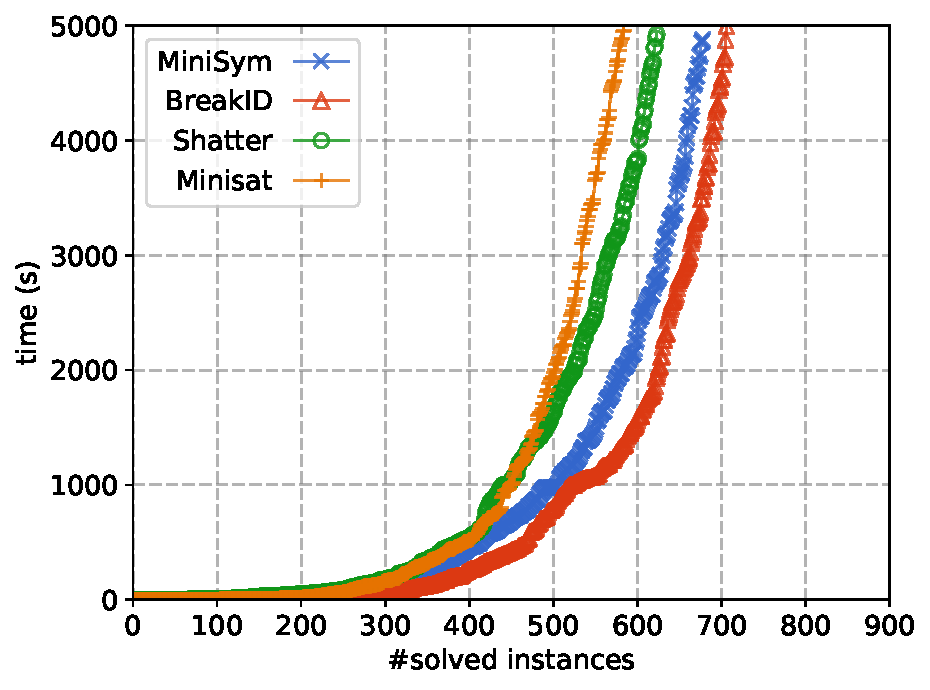
\includegraphics[scale=0.36]{img/saucy-result}}}%
 \qquad
 \subfloat[with \bliss]{{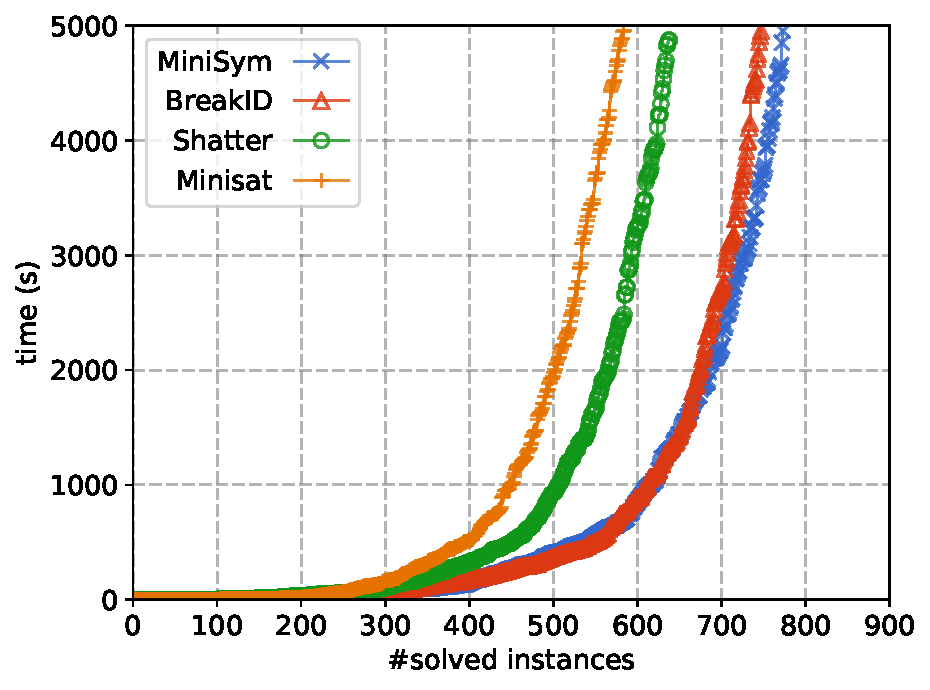
\includegraphics[scale=0.36]{img/bliss-result}}}%
 \caption{cactus plot  total number of instances}%
 \label{fig:cactus}%
\end{figure}

We observe that performances our tool are better with \bliss{} than with
\saucy{} (see fig~\ref{fig:cactus}). We explain it as follows: \saucy{} is
known to compute fewer generators for the group of symmetries than \bliss{}.
Since the larger the symmetries set is, the earlier the detection of an
\emph{evidence} that an assignment is not a \textit{lex-leader} will be, we
generate fewer symmetry-breaking predicates (only the effective ones). This is
shown in Table~\ref{tab:sbp}; \cdclsym{} generates an order of magnitude fewer
predicates than \breakid{}.

\begin{table}[!htbp]
 \resizebox{1 \textwidth}{!}{
  \subfloat[With \saucy]{%
   \begin{tabular}{l|c|c}
    Number of SBPs & \texttt{BreakID}  & \texttt{MiniSym}\\
    \hline
    $\unsat$ (316) & 12\,088\,433  & \cellcolor{gray!30}1\,579\,623 \\
    $\sat$  (312)    & 13\,839\,689  & \  \cellcolor{gray!30}359\,352     
    \label{sbp-saucy}
   \end{tabular}
  }
  \hspace{1em}
  \subfloat[With \bliss]{%
   \begin{tabular}{l|c|c}
    Number of SBPs & \texttt{BreakID}  & \texttt{MiniSym}\\
    \hline
    $\unsat$ (399) &  2\,576\,349 &  \cellcolor{gray!30}913\,339\\
    $\sat$  (320) & 12\,179\,513  & \  \cellcolor{gray!30}457\,452 
    \label{sbp-bliss}
   \end{tabular}
  }
 }
 \vspace*{0.1cm}
 \caption{Comparison of the number of generated SBPs each time \breakid{} and 
  \cdclsym{} both compute a verdict (number of verdicts between parentheses).}
 \label{tab:sbp}
\end{table}

We also conducted experiments on highly symmetrical instances (all variables
are involved in symmetries), whose results are presented
in~\Cref{table:bench2}. The performance of \breakid{} on this benchmark is
explained by a specific optimization for the \emph{total symmetry groups} that
are found in these examples, that is neither implemented in \shatter{} nor in
\cdclsym{}. However, the difference between \breakid{} and \cdclsym{} is rather
thin when using $\bliss{}$. Our tool still outperforms \shatter{} on this
benchmark.

\begin{table}[!htbp]
 \resizebox{1 \textwidth}{!}{
  \subfloat[With \saucy]{%
   \begin{tabular}{l|cccc}
    Benchmark  & \minisat{} & \shatter{} & \breakid{} & \cdclsym{} \\
    \hline
    battleship(6) & \cellcolor{gray!30}\textbf{5} &\cellcolor{gray!30}\textbf{5} & \cellcolor{gray!30}\textbf{5} & \cellcolor{gray!30}\textbf{5}\\
    chnl(6) &  4 & \cellcolor{gray!30}\textbf{6} & \cellcolor{gray!30}\textbf{6} & \cellcolor{gray!30}\textbf{6}\\
    clqcolor(10)  &  3 & 4 & 5 & \cellcolor{gray!30}\textbf{6} \\
    fpga(10) &   6 & \cellcolor{gray!30}\textbf{10} & \cellcolor{gray!30}\textbf{10} & \cellcolor{gray!30}\textbf{10}\\
    hole(24) &   10 & 12 & \cellcolor{gray!30}\textbf{23} & 11\\
    hole shuffle(12)  &  1  & 2 & \cellcolor{gray!30}\textbf{12} & 3\\
    urq(6) &   1  & 2 & \cellcolor{gray!30}\textbf{6} & 2\\
    xorchain(2)  &  1 & 1 & \cellcolor{gray!30}\textbf{2} & \cellcolor{gray!30}\textbf{2} \\
    \hline
    TOTAL & 31 & 42 & \cellcolor{gray!30}\textbf{69} & 45\\
   \end{tabular}
  }
  \hspace{1em}
  \subfloat[With \bliss]{%
   \begin{tabular}{l|cccc}
    Benchmark  & \minisat{} & \shatter{} & \breakid{} & \cdclsym{} \\
    \hline
    battleship(6) & 5 & 5 & 5 & \cellcolor{gray!30}\textbf{6} \\
    chnl(6) &  4 &  \cellcolor{gray!30}\textbf{6} & \cellcolor{gray!30}\textbf{6} & \cellcolor{gray!30}\textbf{6} \\
    clqcolor(10)  &  3 & 5 & 8 & \cellcolor{gray!30}\textbf{10} \\
    fpga(10) &   6 & \cellcolor{gray!30}\textbf{10} & \cellcolor{gray!30}\textbf{10} & \cellcolor{gray!30}\textbf{10} \\
    hole(24) &   10 &\cellcolor{gray!30}\textbf{24} & \cellcolor{gray!30}\textbf{24} & 23 \\
    hole shuffle(12)  &  1  &  3 & \cellcolor{gray!30}\textbf{7} & 4\\
    urq(6) &   1  & 2 & \cellcolor{gray!30}\textbf{6} & 5\\
    xorchain(2)  &  1 & 1 & \cellcolor{gray!30}\textbf{2} & \cellcolor{gray!30}\textbf{2}\\
    \hline
    TOTAL & 31 & 56 & \cellcolor{gray!30}\textbf{68} & 66 \\
   \end{tabular}
  }
 }
 \vspace*{0.1cm}
 \caption{Comparison of the tools on 76 highly symmetric $\unsat$ problems.}
 \label{table:bench2}
\end{table}

\section{Some optimization}
Dynamic usage of symmetry properties allows the solver to adapt classical heuristics and symmetry based one on-the-fly.
For example, some restart heuristics are based on the number of conflicts, taking into account injection of esbp may impact
the performance of the overall SAT solver. 
\subsection{Adapt heuristics dynamically}
Other heuristics on the symmetry handling may increase the performance. We present here some of them.
In some cases, multiple permutations can be reducers at the same time, and each one generates different symmetry breaking constraints.
The backtrack and the pruning capacity depends heavily on the chosen constraint. In our library, the first reducer permutation generates the \textit{esbp}. 
Another point concerns the injection of the symmetry breaking predicates. Two choices are possible, first,
before the unit propagation and second, at the end of the propagation. This choice will impact the solver behavior.
In the first case, esbp takes the lead over the classical conflict (if it occurs). Conversely, in the second case, the classical conflict
takes the lead over esbp. This can be especially useful on SAT problems because esbp can eliminate non lex-leader SAT assignment.
To emphasize this behavior, the conflict of the esbp can be ignored in the sense that the conflict clause is just added into the clause database and so will participate to the next unit propagation. This gives to the solver the ability to find a solution symmetrical branch but avoid to get multiple times on non-minimal part of search. It can be useful if we know in advance that the problem is satisfiable.

\subsection{Change the Order Dynamically}
As seen before, the ordering relationship between variables influence the minimal value of each orbit (lex-leader) and the generated constraints. The symmetry controller is "waiting" for the solver that assigns the variables that allows it to decide if the current assignment is the lex-leader.
The main idea to change dynamically the order, and so the lex-leader, is that the symmetry breaking order follows the decision heuristics of the solver, then the symmetry controller can decide quickly if the current assignment is minimal.
Changing this order dynamically is possible with some requirements: all esbps  and all deduced 
clauses from a symmetry breaking predicates need to be removed. If these constraints are not deleted,
the correctness of the algorithm is not guaranteed.
% inconsistencies may appear and a satisfiable problem become unsatisfiable. 
%So, changing this order will force the solver to forget all learned clauses that makes the strength of CDCL solver. 

\subsection{Impact of the sign in variable ordering}
With the same variables ordering, swapping the value thus, $\true < \false$ or $\false < \true$
may impact drastically the performance of the solver.
To illustrate it, consider the pigeonhole problem with 100 holes and 101 pigeons with 
the increasing order of the variables and change only the sign.
With  $\false < \true$, the solver generates 20\,619 esbps, and takes 13.8 seconds to solve it.
With the reverse order ($\true < \false$), it generates 33\,263 esbps and solves it in 93.4 seconds.
\Cref{table:compare_sign_order} shows this difference on 500 symmetric instances with
a scatter plot that compares the same variable order with $\true < \false$ and $\false < \true$,
 \texttt{MiniSymFT} is the solver in which $\false < \true$, and  \texttt{MiniSymTF} is the solver in which $\true < \false$.
On the left, we compare the computation time of the solver. 
As we can observe \texttt{MiniSymTF} is more efficient on some $\unsat$ instances (red points in the figure).
The right figure shows the number of generated esbp by solvers in a log scale. On the large majority of instances, they generate 
approximately the same number of esbps. But the difference can be an order of magnitude higher. This can be due to the time of
execution of the solver and/or the impact of the sign of the constraints.

\clearpage
\begin{figure}[!htbp]
 \subfloat[Time]{%
  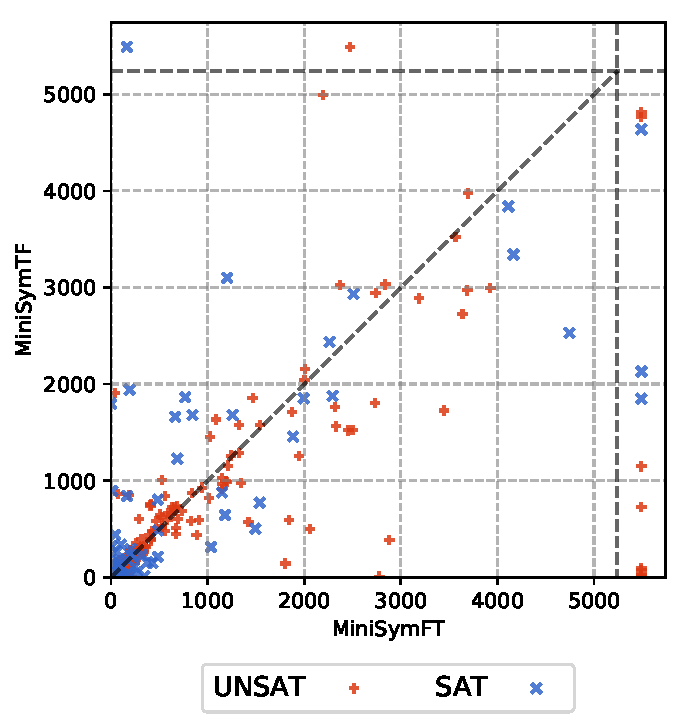
\includegraphics[width=.3\textheight]{img/scatter_compare}%
 }
 \hspace{1em}
 \subfloat[Number of esbp]{%
  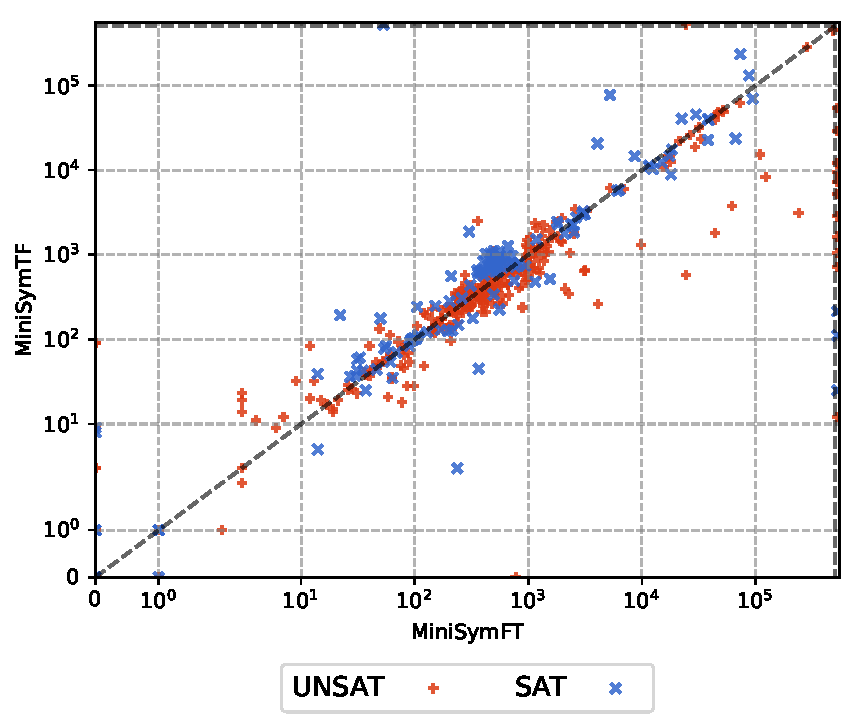
\includegraphics[width=.375\textheight]{img/scatter_esbp_compare}%
 }
 \vspace*{0.1cm}
 \caption{Comparison of the order with different signs on 500 symmetric instances.}
 \label{table:compare_sign_order}
\end{figure}


\texttt{MiniSymTF} is generally better and is the default choice in the library.
If it is running on a specific application, reverse order can be chosen if it performs better.


\section{Conclusion}
SymmSAT uses same the principles as static symmetry breaking approaches but operates dynamically by 
injecting \textit{effective symmetry breaking} during the search.
This overcomes the main problem of the static approaches, i.e. that they
generate many \textit{sbps} that are not effective in the solving (size of the
generated formulas, overburden of the unit propagation procedure, etc.).
The idea we brought is to break symmetries \emph{on-the-fly}: when the current
partial assignment cannot be a prefix of a \textit{lex-leader} (of an orbit),
an \textit{esbp} that prunes this forbidden assignment and all its extensions is generated. 
This approach is implemented in the C++ library called \libdsb{}. It is an
off-the-shelf component that can be interfaced with virtually any CDCL SAT
solver. \libdsb{} is released under GPL license and is available at
\url{https://github.com/lip6/cosy}.
 
The extensive evaluation of our approach on the symmetric formulas of the 
 SAT contests from 2012 to 2017 shows that it outperforms the state-of-the-art techniques, in
particular on unsatisfiable instances, in which the whole search space must be explored.
\setcounter{mtc}{5} 
\chapter{Compose dynamic symmetry handling}
\minitoc
\section{Composition of SP and SymmSAT}
Recently, we developed an approach that reuses the
principles of the static approaches, but operates dynamically (namely, the effective symmetry breaking approach~\cite{metin2018cdclsym}):
 the symmetries are broken during the search process without any pre-generation of the \textit{sbp}. The main
advantage of this technique is to cope with the heavy (and potentially
blocking) pre-generation phase of the static-based approaches. It also gives
more flexibility for adjusting some parameters on the fly. 
Nevertheless, we also observed that many formulas easily solved by the pure
dynamic approaches remained unsolvable by our approach and vice versa. This is
particularly true with the \textit{symmetry propagation} technique developed by
Devriendt et al.~\cite{Devriendt12}.
Hence, our goal is to explore the composition of our algorithm with the  \textit{symmetry propagation} technique in
a new approach that would mix the advantages of the two classes of techniques while alleviating their drawbacks. At first sight,
the two approaches appear to be orthogonal, and hence could be mixed easily. However, as we show in the rest of this section,
this is not completely true: both theoretical and practical issues have to be analyzed and solved to get a
running complementary. 
Since the approach based on symmetry propagation (later called SPA) focuses on
accelerating the tree traversal and the approach based on effective symmetry
breaking (later called ESBA) targets to prune the tree traversal, the question of combining these approaches, to solve a formula $\varphi$, can
be reformulated as: 
\begin{center}
 \textit{is it possible to accelerate the traversal while pruning the tree?}
\end{center}
\subsection{Theoretical foundations}
\label{sec:tf}
To answer the previous questions, we analyze the evolution of $\varphi$ during
its solving. In ESBA, $\varphi$ evolves, incrementally, to an
equi-satisfiable formula of the form $\varphi \equiv \varphi \cup \varphi_e
\cup \varphi_d$, where $\varphi_e$ is a set of injected esbps and $\varphi_d$
is a set of deduced clauses (logical consequences). Both sets are modified continuously during the solving. Hence, to be able to compose ESBA with SPA, we have to consider the symmetries of $\varphi^\prime=\varphi \cup \varphi_e \cup \varphi_d$ as
allowed permutations in place of those of $\varphi$.
A first naive solution could be to recompute, dynamically, the set of symmetries of $\varphi
\cup \varphi_e \cup \varphi_d$ for each new $\varphi_e \cup \varphi_d$, but
this would be an intractable solution generating a huge complexity. 
A  computationally less expensive solution would be to keep track of all globally unbroken symmetries as the clauses of $\varphi_e$ are injected during the solving process: considering formula $\varphi$ and 
a set of esbps $\varphi_e$ then the set of global unbroken symmetries is:
$$GUS = \underset{\omega_e \in \varphi_e}{\bigcap}Stab(\omega_e) \cap S(\varphi)$$
 Where  $Stab(\omega_e)=\{g \in \Group{\Vars}\mid
\omega_e=g.\omega_e\}$ is the stabilizer set of $\omega_e$ and $S(\varphi)$ is the set of symmetries of $\varphi$. 
Since $\varphi \cup \varphi_e  \models \varphi_d$, then $GUS$ is a valid set of symmetries for $\varphi \cup \varphi_e \cup \varphi_d$.
Then, (1) each time a new set of esbp clauses is added, its stabilizer will be used to reduce $GUS$;
(2) conversely, when a set of esbp clauses is reduced\footnote{In classical CDCL algorithm, this can be due to a back-jump or a restart.},
$GUS$ cannot be enlarged by the recovered broken symmetries because of the retrieved set:
\textit{at that point, we do not know which symmetries become valid}! 
As a consequence, the set of globally unbroken symmetries will converge very quickly to the empty set. 
At this point, SPA will be blocked for the rest of the solving process without any chance to recover.
 Therefore, this solution is of limited interest in practice.
We propose here to improve the aforementioned solution by alleviating the issue cited in point (2).
We first present the intuition, then we will detail and formalize it. 
%The idea here is to keep track of particular symmetries for each clause. For a deduced clause, this set of symmetries captures which esbp's were involved in a deduced clause's derivation. The intersection of these sets is a superset of the globally unbroken symmetries, and a strict superset after clause deletion.
Consider formula $\varphi^\prime$ as before. It can be rewritten as:
$$\varphi^\prime=\varphi \, \underset{i}{\bigcup}(\varphi_e^i \cup \varphi_d^i) \text{ , such that } \varphi_e \cup \varphi_d = \underset{i}{\bigcup}(\varphi_e^i \cup \varphi_d^i) \text{ and } \varphi \cup \varphi_e^i \models \varphi_d^i  \text{ for all } i$$
So, $GUS_i = \underset{\omega_e \in \varphi_e^i}{\bigcap}Stab(\omega_e) \cap S(\varphi)$ is a valid set of symmetries for the sub-formula $\varphi \cup \varphi_e^i \cup \varphi_d^i$, and $GUS$ can be obtained by $GUS = \underset{i}{\bigcap} GUS_i$. If some esbp clauses are added to $\varphi^\prime$, then the new $GUS$ is computed as described in (1). The novelty here comes with the retrieval of some set of clauses: by keeping track of the symmetries associated to each sub-formula ($GUS_i$), it is now easy to recompute a valid set of symmetries for $\varphi^\prime$ when some set
$\varphi_e^k \cup \varphi_d^k$ is retrieved. It suffices to operate the intersection on the valid symmetries of the rest of the sub-formulas: $GUS = \underset{i \neq k}{\bigcap} GUS_i$.
Just say your approach keeps track of a set of particular symmetries for each clause. For a deduced clause, this set of symmetry captures which esbp's were involved in a deduced clause's derivation. The intersection of these sets is a superset of the globally unbroken symmetries, and a strict superset after clause deletion.
\subsection{Local Symmetries}
The general and formal framework that embodies the above idea is given by the following. It first relies on the notion of \textit{local symmetries} that we introduce in \cref{def:ls}.
\begin{definition}
 \label{def:ls}
 Let $\varphi$ be a formula. We define $L_{\omega,\varphi}$, 
 the set of \textit{local symmetries} for a clause $\omega$, and with respect to 
 a formula $\varphi$, as follows:
 
 $$L_{\omega,\varphi}=\{g \in \Group{\Vars}\mid \varphi \models g.\omega\}$$
\end{definition}
$L_{\omega,\varphi}$ is local since the set of permutations applies locally to
$\omega$. It is then straightforward to deduce the next proposition that gives us a
practical framework to compute, incrementally, a set of symmetries for a
formula (by using the intersection of all local symmetries).
\begin{proposition}
 \label{prop:gls-prop}
 Let $\varphi$ be a formula. Then,  $\underset{\omega \in \varphi}{\bigcap}L_{\omega,\varphi} 
 \subseteq S(\varphi)$.
\end{proposition}
\begin{proof}
 Let $\varphi$ be a formula. Then, $\forall \omega \in \varphi, \forall g \in L_{\omega,\varphi}, \varphi \models g.\varphi $. So, $\forall g \in \underset{\omega \in \varphi}{\bigcap}L_{\omega,\varphi}, \varphi \models g.\varphi$. This is combined with the fact that the number of satisfying assignments for a formula is not changed by permuting the variables of the formula, we have $g.\varphi \models \varphi$. Hence $\varphi \equiv g.\varphi$, and $g \in S(\varphi)$ (by definition). 
\end{proof}
Using this proposition, it becomes easy to reconsider the symmetries
on-the-fly: each time a new clause $\omega$ is added to the formula $\varphi$,
we can just operate an intersection between $L_{\omega,\varphi}$ and
$\underset{\omega^\prime \in \varphi}{\bigcap}L_{\omega^\prime,\varphi}$ to get
a new set of valid symmetries for $\varphi \cup \{\omega\}$.
\medskip
Proposition \ref{prop:lsc-prop} establishes the relationship between the local symmetries of a deduced clause and those of the set of clauses that allow its derivation. 
\begin{proposition}
 \label{prop:lsc-prop}
 Let $\varphi_1$ and $\varphi_2$ be two formulas, with $\varphi_2 \subseteq \varphi_1$. 
 Let $\omega$ be a clause such that $\varphi_2 \models \omega$. Then, 
 $(\underset{\omega^\prime \in \varphi_2}{\bigcap}L_{\omega^\prime,\varphi_1})
 \cup Stab(\omega) \subseteq L_{\omega,\varphi_1}$;
\end{proposition} 
\begin{proof}
 Let us consider a clause $\omega$ and a permutation $g \in 
 (\underset{\omega^\prime \in \varphi_2}{\bigcap}L_{\omega^\prime,\varphi_1})
 \cup Stab(\omega)$.
 Since, $\varphi_2 \models \omega$, then  $g.\varphi_2 \models g.\omega$. Since $\varphi_1 \models \varphi_2 (\varphi_2 \subseteq \varphi_1)$, and 
 $g \in 
 (\underset{\omega^\prime \in \varphi_2}{\bigcap}L_{\omega^\prime,\varphi_1})
 \cup Stab(\omega)$, then we have $\varphi_1 \models g.\varphi_2$ (from Def.~\ref{def:ls}). Hence, $\varphi_1 \models g.\varphi_2 \models g.\omega$, and then, $g \in L_{\omega,\varphi_1}$ (by definition). 
\end{proof}
\subsection{Algorithm}
This section shows how to integrate the propositions developed in the previous
section as the basis of our combo approach in a concrete
Conflict-Driven Clause Learning (CDCL)-like solver.
First recall the algorithm of symmetry propagation used for the combination of two approaches.
	\begin{algorithm}[!htbp]
		
			\small	
		\SetKwProg{Fn}{function}{}{}
		\SetKwData{C}{symController}
		\SetKwData{CSP}{spController}
		\SetKwFunction{CDCL}{CDCLSymSp}
		\SetKwFunction{unitPropagation}{unitPropagation}
		\SetKwFunction{symPropagation}{symPropagation}
		\SetKwFunction{updateSymmetries}{updateActiveSymmetries}
		\SetKwFunction{cancelSymmetries}{cancelActiveSymmetries}
		\SetKwFunction{analyzeConflict}{analyzeConflict}
		\SetKwFunction{isSymmetryConflict}{isSymmetryConflict}
		\SetKwFunction{assignNewLiteral}{assignDecisionLiteral}
		\SetKwFunction{backjumpPolicy}{backjumpAndRestartPolicies}
		
	
	\Fn{
		\CDCL{$\varphi$: CNF formula, \colorsp{\CSP : symmetry propagation controller}}\\
		$\quad\quad$\textbf{returns} $\true$ if $\varphi$ is \sat and $\false$ otherwise
	}
	{
		$dl \gets 0$ \tcp*{Current decision level}
		$\alpha \gets \emptyset$\;
		\While{not all variables are assigned}{
			$isConflict \gets$ \unitPropagation{}  \
			\colorsp{$\wedge$ \CSP.\symPropagation{}}\;	\label{algo:cdclsp:symprop}
			\If{$isConflict$}{
				\If{dl = 0}{
					\Return \false
					\tcp*{$\varphi$ is $\unsat$}
				}
				$\omega \gets$ \analyzeConflict{}\;
				$dl \gets$ \backjumpPolicy{}\;
				$\varphi \gets \varphi \cup \{\omega$\} \;
				\colorsp{\CSP.\cancelSymmetries{}}\; \label{algo:cdclsp:cancel}	
			}
			\Else{
				$\alpha \gets \alpha\, \cup $ \assignNewLiteral{}\; 
				$dl \gets dl+1$\;
				\colorsp{\CSP.\updateSymmetries{}}\; \label{algo:cdclsp:update}
			}
		}
		\Return \true
		\tcp*{$\varphi$ is $\sat$}
	}
	\caption{The {\cdclsp} algorithm. Blue (or grey) parts denote additions to {\cdcl}.}
	\label{algo:cdclsp}
	
\end{algorithm}


{\cdclsp} (see Algorithm~\ref{algo:cdclsp}) implements SPA, and also has a
structure similar to the one of {\cdcl}. In this algorithm, the symmetry
propagation actions are executed by the controller component (\texttt{spController})
through a call to the function \texttt{symPropagation} (\cref{algo:cdclsp:symprop}). This
propagation is allowed only if the conditions %of Proposition \ref{prop:ws-prop}
are met. Such conditions are evaluated by tracking on-the-fly the status of the
symmetries. This is implemented by functions \texttt{updateSymmetries} (\cref{algo:cdclsp:update})
and \texttt{cancelSymmetries} (\cref{algo:cdclsp:cancel}).

\begin{algorithm}[!htbp]	
	\small	
	\SetKwProg{Fn}{function}{}{}
	\SetKwData{C}{symController}
	\SetKwData{CSP}{spController}
	\SetKwFunction{CDCL}{CDCLSymSp}
	\SetKwFunction{unitPropagation}{unitPropagation}

	\SetKwFunction{symPropagation}{symPropagation}
	
	\SetKwFunction{updateSymmetries}{updateActiveSymmetriesSym}
	
	\SetKwFunction{cancelSymmetriesSym}{cancelActiveSymmetriesSym}
	
	\SetKwFunction{updateLocSymmetries}{updateLocalSymmetries}
	
	\SetKwFunction{analyzeConflict}{analyzeConflictSymSp}

	
	\SetKwFunction{isSymmetryConflict}{isSymmetryConflict}
	\SetKwFunction{assignNewLiteral}{assignDecisionLiteral}

	\SetKwFunction{backjumpPolicy}{backjumpAndRestartPolicies}

	\SetKwFunction{isNotMinimal}{isNotLexLeader}
	\SetKwFunction{SBP}{generateEsbpSp}
	\SetKwFunction{notifyAssigned}{updateAssign}
	\SetKwFunction{notifyCancelled}{updateCancel}


	
	\Fn{
		\CDCL{$\varphi$: CNF formula, \colorsym{\C: symmetry controller},\\
			 \hspace{11em} \colorsp{\CSP : symmetry propagation controller}}\\
		$\quad\quad$\textbf{returns} $\true$ if $\varphi$ is $\sat$ and $\false$ otherwise
	}
	{

		$dl \gets 0$ \tcp*{Current decision level}
		$\alpha \gets \emptyset$\;
		\While{not all variables are assigned}{
			
			$isConflict \gets$ \unitPropagation{}  \colorsp{$\land$ \CSP.\symPropagation{}}\;\label{algo:sym_prop}
			\colorsym{\C.\notifyAssigned{$\alpha$}\;}
			\colorsym{$isReduced \gets$ \C.\isNotMinimal{$\alpha$}\;}
			
			\If{$isConflict$ \colorsym{$\vee\, isReduced$}}{
				\If{dl = 0}{
					\Return \false
					\tcp*{$\varphi$ is $\unsat$}
				}
				
				\If{$isConflict$}{\label{algo:start_stab}
					
					\colorbox{gray!30}{$\langle\omega, L = \underset{\omega' \in \varphi_1}{\bigcap}L_{\omega',\varphi_1} \cup Stab(\omega)\rangle \gets$ \analyzeConflict{}\;}
				}
				\Else {
					\colorbox{gray!30}{$\langle\omega, L = Stab(\omega)\rangle \gets$ \C.\SBP{$\alpha$}\;}
				}\label{algo:end_stab}		
				
				
				$(dl,\alpha) \gets$ \backjumpPolicy{}\;
				$\varphi \gets \varphi \cup \{\omega$\} \;
				
				\colorsym{\C.\notifyCancelled{$\alpha$}}\;
				\colorbox{gray!30}{\CSP.\cancelSymmetriesSym{}}\;\label{algo:symsp:cancel}
				\colorbox{gray!30}{\CSP.\updateLocSymmetries{L}\;}\label{algo:symsp:updateloc}
				
			}
			\Else{
				$\alpha \gets \alpha\, \cup $ \assignNewLiteral{}\; 
				$dl \gets dl+1$\;
				\colorbox{gray!30}{\CSP.\updateSymmetries{}}\;\label{algo:symsp:updateact}
			}
		}
		\Return \true
		\tcp*{$\varphi$ is $\sat$}
	}
	\caption{The {\cdclsymsp} algorithm. Additions derived
		from {\cdclsym} and {\cdclsp} are reported in red and blue (or grey). Additions
		due to the composition of the two algorithms are reported with a gray
		background.}
	\label{algo:cdclSYMSP}
\end{algorithm}
 
The algorithm we propose for the composed approach is presented in
algorithm~\ref{algo:cdclSYMSP}. 
%Lines $3$-$10$, $15$-$17$ and $20$-$22$ correspond to the exact union of {\cdclsym} and {\cdclsp}. 
Let us detail the critical points.
\begin{itemize}[topsep=2pt]
 \item \Cref{algo:start_stab,algo:end_stab}: when a conflict is detected, then the analyzing
 procedure is triggered. According to Proposition \ref{prop:lsc-prop}, the
 generated conflicting clause $\omega$, should be associated with the
 computation of its set of local symmetries. Thus, we update the classical
 \texttt{analyzeConflict} procedure to \texttt{analyzeConflictSymSp} that produces such
 a set: $\varphi_1$ contains all the clauses that are used to derive $\omega$\footnote{These are clauses of the \textit{conflict side} of the implication graph when applying the classical conflict analysis algorithm.}. So, at the end of the conflict analysis we operate the intersection of a local symmetry of these clauses to get the set of local symmetries of $\omega$. We can thus complete this set with the stabilizer set (see as Proposition \ref{prop:lsc-prop}).
 
 In the classical algorithm of symmSAT, when a non lex-leader assignment is detected
 , then the esbp generation function, \texttt{generateEsbp}, is
 called. In the new algorithm this function is replaced by a new one called
 \texttt{generateEsbpSp}. In addition to compute the esbp clause $\omega$, it
 produces the stabilizer set of $\omega$\footnote{The only allowed
  local symmetries in case of an esbp, according to point~2 of
  section~\ref{sec:pc}.}.
 
 \item \Cref{algo:symsp:cancel}: \texttt{cancelActiveSymmetriesSym} extends function \texttt{cancelActiveSymmetries} of Algorithm~\ref{algo:cdclsp} with the additional reactivation of the symmetries that have been broken (deactivated) by ESBPA. Technically speaking, each time a deduced literal is unassigned, all symmetries that became inactive because of its assignment (see \texttt{updateLocalSymmetries} and \texttt{updateActiveSymmetriesSym} functions below) are \textit{reactivated}.
 
 \item \Cref{algo:symsp:updateloc}: \texttt{updateLocalSymmetries} is a new function of
 $\texttt{spController}$. It is responsible of updating the status of the manipulated
 symmetries so that only those respecting Proposition \ref{prop:gls-prop} are
 active each time the \texttt{symPropagation} function is called. Technically speaking, each symmetry of the complement set (to $S(\varphi)$) of the set $L$ is marked \textit{inactive} (it is a broken symmetry), if it is not already marked so. Here, the asserting literal of clause $\omega$ becomes responsible of this deactivation. 
 
 \item \Cref{algo:symsp:updateact}: \texttt{updateActiveSymmetriesSym} extends function \texttt{updateActiveSymmetries} of algorithm~\ref{algo:cdclsp}. The reason clause, $\omega_l$, of each propagated literal, $l$, by the \texttt{unitPropagation} function is analyzed. Each symmetry of the complement set (to $S(\varphi)$) of the set local symmetries of $\omega_r$ is marked \textit{inactive}, if it is not already marked so. $l$ becomes responsible of this deactivation. 
\end{itemize}
\subsection{Implementation}
We have implemented our combo on top of the
\texttt{minisat-SPFS}\footnote{https://github.com/JoD/minisat-SPFS} solver,
developed by the authors of SPA.
This choice has been influenced by two points: (1) take advantage of the
expertise used to implement the original SPA method; (2) the easiness of
integrating our implementation of ESBA to any CDCL-like solver because it is an
off-the-shelf library\footnote{This library is released under GPL v3 license,
see \url{https://github.com/lip6/cosy}.}.
However, this choice has the drawback of doubling the representation of
symmetries. This can be a hard limit to treat certain big problems from the
memory point of view.
The implemented combo solver can be found at:\\
\mbox{\url{https://github.com/lip6/minisat-SymSp}}
\subsection{Evaluation}
This section compares our combo approach against ESBA and SPA. All experiments
have been performed with a modified version of the well-known \minisat{} solver \cite{een2003extensible}: \texttt{minisat-Sp}, for
SPA; \texttt{minisat-Sym}, for ESBA; and \texttt{minisat-SymSP}, for the
combo. Symmetries of the SAT problems have been computed by
\bliss{}~\cite{JunttilaKaski:ALENEX2007}.
We selected from the last seven editions of the SAT contest
\cite{jarvisalo2012international}, the CNF problems for which \bliss{} finds
some symmetries that could be computed in at most $1000s$ of CPU time. We
obtained a total of $1400$ SAT problems (discarding repetitions) out of the
$4000$ proposed by the seven editions of the contest.
\begin{table}\footnotesize
 \centering
 % \resizebox{1 \textwidth}{!}{
 \begin{tabular}{l|ccc}
  \toprule
  Benchmark  &\texttt{minisat-Sp} & \texttt{minisat-Sym} & \texttt{minisat-SymSP}\\
  \hline 
  Generators 0–20 (704) & 194&197&\cellcolor{gray!30,}\textbf{198}\\
  Generators 20–40 (136) & 33&\cellcolor{gray!30}\textbf{34}&\cellcolor{gray!30}\textbf{34}\\
  Generators 40–60 (141) & 28&28&\cellcolor{gray!30}\textbf{29}\\
  Generators 60–80 (168) & \cellcolor{gray!30}\textbf{65}&64&\cellcolor{gray!30}\textbf{65}\\
  Generators 80–100 (51) & 28&\cellcolor{gray!30}\textbf{34}&\cellcolor{gray!30}\textbf{34}\\
  Generators  \textgreater100 (200) & 58&59&\cellcolor{gray!30}\textbf{60}\\
  \hline 
  TOTAL no dup (1400) & 406 & 416 & \cellcolor{gray!30,}\textbf{420}\\
  \bottomrule
 \end{tabular}
 % }
 \caption{Comparison of the number of SAT problems solved by each approach.}
 \label{tab:sat}
\end{table}
\begin{table}\footnotesize
 \centering
 % \resizebox{1 \textwidth}{!}{
 \begin{tabular}{l|ccc}
  \toprule
  Benchmark  &\texttt{minisat-Sp} & \texttt{minisat-Sym} & \texttt{minisat-SymSP}\\
  \hline 
  Generators 0–20 (704) & \cellcolor{gray!30,}\textbf{233}&220&226\\
  Generators 20–40 (136) & 50&\cellcolor{gray!30}\textbf{54}&\cellcolor{gray!30}\textbf{54}\\
  Generators 40–60 (141) & 75&\cellcolor{gray!30}\textbf{83}&\cellcolor{gray!30}\textbf{83}\\
  Generators 60–80 (168) & \cellcolor{gray!30}\textbf{11}&\cellcolor{gray!30}\textbf{11}&10\\
  Generators 80–100 (51) & \cellcolor{gray!30}\textbf{11}&\cellcolor{gray!30}\textbf{11}&\cellcolor{gray!30}\textbf{11}\\
  Generators \textgreater100 (200) & 90&\cellcolor{gray!30,}\textbf{109}&107\\
  \hline 
  TOTAL no dup (1400) & 470&488&\cellcolor{gray!30,}\textbf{491}\\
  \bottomrule
 \end{tabular}
 % }
 \caption{Comparison of the number of UNSAT problems solved by each approach.}
 \label{tab:unsat}
\end{table}
All experiments have been conducted using the following settings: each solver
has been run once on each problem, with a time-out of 7200 seconds (including
the execution time of symmetry generation) and limited to 64 GB of memory.
Experiments were executed on a computer with an Intel® Xeon® Gold 6148 CPU
@ 2.40 GHz featuring 80 cores and 1500 GB of memory, running a Linux 4.17.18,
along with g++ compiler version 8.2.
Tables \ref{tab:sat} and \ref{tab:unsat} present the obtained results for SAT
and UNSAT problems respectively. The first column of each table lists the
classes of problems on which we operated our experiments: we classify the
problems according to the number of symmetries they admit. A line noted
``generators X-Y (Z)'' groups the Z problems having between X and Y generators
(i.e., symmetries). Other columns show the number of solved problems for each
approach.
Globally, we observe that the combo approach can be effective in many classes
of symmetric problems. For SAT problems, the combo has better results than the
two other approaches (4 more SAT problems when compared to the best of the two
others) and this is despite the significant cost paid for the tracking of the
symmetries' status. When looking at the UNSAT problems, things are more
mitigated. Although, the total number of solver problems is greater than the
best of the two others, we believe that the cost for tracking the symmetries'
status has an impact on the performances. This can be observed on the first and
last lines of Tables~\ref{tab:unsat}: when the number of generators is small
(first line), the ESBA benefits greatly from the SPA. When the number of
generators is high (last line), we see a small loss of the combo with respect
to ESBA. It is also worth noting that the combo approach solved \textbf{8} problems 
that could not be handled by ESBA nor SPA.
%These observations are confirmed by the scatter plots of Fig.\textcolor{red}{X}.
\begin{table}[!htbp]
 \begin{center}
  \resizebox{0.5 \textwidth}{!}{
   \begin{tabular}{lcc}
    \hline
    Solvers                  &    PAR2 (1400) &   CTI (825) \\
    \hline
    \texttt{minisat-SymSp}   & \cellcolor{gray!30}{5,653,089} &      614,856 \\
    \texttt{minisat-Sym}             & 5,682,892 &      \cellcolor{gray!30,}{584,868} \\
    \texttt{minisat-Sp}             & 6,026,840 &      612,638 \\
    \hline
   \end{tabular}
  }
 \end{center}
 \caption{Comparison of PAR-2 and CTI times (in seconds) of the global solving.}
 \label{tab:global}
\end{table}
Table~\ref{tab:global} compares the different techniques with respect to the
PAR-2 and the CTI time measures. PAR-2 is the official ranking measure used in
the yearly SAT contests~\cite{jarvisalo2012international}. CTI measures the
Cumulative solving Time of the problem Intersection (i.e., 825 problems solved
by all solvers). While PAR-2 value gives a global indication on the
effectiveness of an approach, CTI is a good mean to evaluate its speed compared
to other approaches.
Hence, we observe that the combo has a better PAR-2 score, and this shows its
effectiveness. However, it is the least fast when coming to solved intersection.
This is clearly due to the double cost paid for tracking the symmetries' status
(one for ESBA and the other for SPA). Having a unified management of
symmetries tracking would probably reduce this cost.
\begin{center}
\begin{figure}[!htbp]
 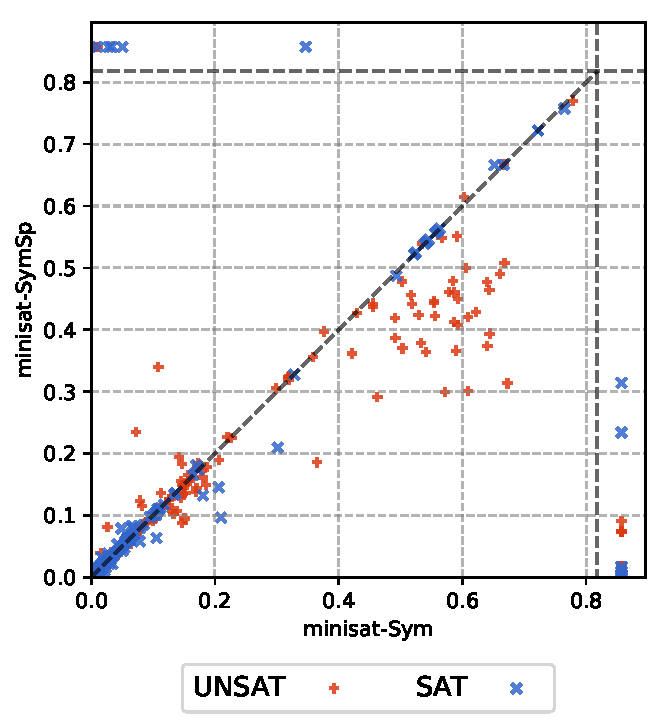
\includegraphics[scale=0.5]{img/full-INFGB-ratio-vscosy.pdf}
 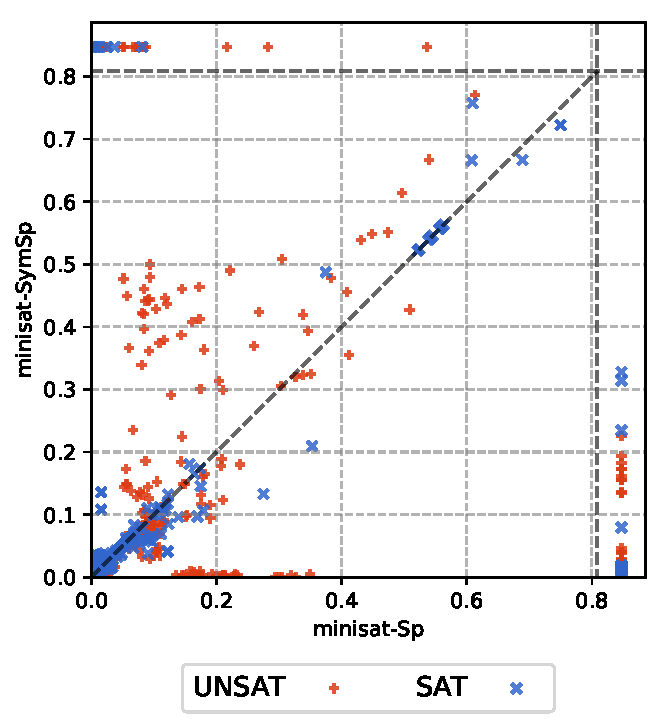
\includegraphics[scale=0.5]{img/full-INFGB-ratio-vsspfs.pdf}
 \caption{Comparison of the ratio between the number of decisions and the number of propagation for the combo w.r.t. ESBA and SPA.}
 \label{fig:ratio}
\end{figure}
\end{center}
To go further in our analyze, we also compare the ratio between the number of
decisions and the number of propagation. This is a fair measure to assess the
quality of a SAT solving approach: if the ratio is small, then this means that
the developed algorithm is producing more deduced facts than making guesses,
which is the best way to conclude quickly on a problem!
The scatter plots of Fig.\ref{fig:ratio} show a comparison between the
aforementioned ratios. When comparing \texttt{minisat-Sp} to
\texttt{minisat-SymSp} (right hand side scatter plot), we observe that the
ratio goes in favor of \texttt{minisat-Sp} for the problems solved by both
approaches. This is an expected result since the main objective of SPA is to
minimize the number of decisions while augmenting the number of propagation.
What is important to underline here is highlighted on the left hand side
scatter plot: on a large majority of UNSAT problems, the ratio goes in favor
of \texttt{minisat-SymSp} w.r.t. \texttt{minisat-Sym}. This confirms the
positive impact of SPA when applied in conjunction with ESBA.
\section{Another combo approach}
Introducing local symmetries allow us to use it with another dynamic approach : 
\textit{Symmetry Explanation Learning} (SEL). It computes the symmetrical learning clause and
include it in the solver clauses when it can be used in the unit propagation or leads to a conflict.
With local symmetries, each clause has a set of allowed symmetries, when a symmetry wants to 
add a symmetrical clause, it suffices to check if this permutation belongs to local symmetries.
\hakan{Naive approach no stab .}
 
\section{Exploitation of local symmetries}
Local symmetries seen previously allows to exploit symmetries in different ways.
Effectively, we can consider symmetries on a part of the problem. Only clauses that are really used
by the solver i.e in the implication graph can be processed.
To obtain the symmetries of the current sub problem is the intersection of local symmetries.

\chapter{Conclusion and Future Works}\label{chap:conclu}



In this thesis, we have presented approaches to increase the performance of solving 
Boolean satisfiability problem (SAT) in presence of symmetries. 
Symmetries are natural things that can be found in different class of problems like
graph coloring problems, fpga routing, etc.
The presence of symmetry in a problem hinders the performance of the solver. It forces
the solver to explore every symmetric branch of the search tree and will face to a combinatorial explosion.
Some trivial question for a human, like Can 100 pigeons fit in 99 holes?,
where each pigeon (hole) are symmetric becomes impossible for a solver. 

%It will explore each pair of pigeon, hole and cannot solve this problem.

To deal with symmetries in problems, two approaches of symmetry breaking exists (see \Cref{chap:symmetryinsat}).
The first one namely called static symmetry breaking approach acts as a preprocessor that augment the initial
problem to prune symmetrical assignments of the search tree. The second one namely called dynamic symmetry breaking 
acts during the solving of the solver. Like in the static approach, it can  prune the symmetrical assignment of the 
search tree or accelerate its traversal using symmetrical facts.
Each approach has its weaknesses and strengths. However, some highly symmetrical instances cannot be solved with
state-of-the-art approaches. This thesis will try to take the best of different approaches to solve 
the hard one.


%This thesis presents novel algorithm to deal with SAT problem in presence of symmetries.
%After a study of the literature on the SAT solving (see \Cref{chap:preliminaries}), and the study of existing 
%approaches to deal with symmetries in SAT (see \Cref{chap:symmetryinsat}). We highlight the strength and weaknesses of these approaches. 
%
%To deal with symmetries, we study the syntactical 
%symmetry detection and the symmetry exploitation.
%

Our first symmetry based approach (see \Cref{chap:symmSAT})introduces the notion of effective symmetry breaking predicates (esbp)
that borrows the principle of static symmetry breaking approach but operating dynamically\cite{metin2018cdclsym}.
This approach overcomes the blow up caused by the pre-generation of \textit{sbp} in the state-of-the-art 
static approaches. The extensive evaluation shows that our approach improves on state-of-the-art static 
symmetry breaking approaches.
The method is encapsulated in a library called $\libdsb$ and can be integrated easily to any
CDCL-like SAT solvers. It is released under GPL-v3 license and is available at \url{https://github.com/lip6/cosy}.

Though easy to use and effective, this method cannot handle some problems that are easily solved by other
dynamic symmetry breaking approach like Symmetry Propagation (SP)~\cite{Devriendt12}.
\Cref{chap:compose} presents our second contribution that aims to combine two dynamic symmetry breaking approach, our first algorithm  with the SP approach. In terms of performance, the combined version not brings big difference
compared to the use of esbp. Nevertheless it can solve few instances that cannot be solved with previous approaches.
Overall,  this  work  answers  to  the  precise  question: "Is is possible to accelerate the traversal while pruning the tree
with symmetries?".We clearly show that the answer is yes, thanks to the introduced theoretical notion of local symmetries.


%This approach use a new
%
%This approach can solve few set of instances that
%cannot be solved with our works.
%
%that are %The first 
%In \Cref{chap:symmSAT}, we develop $\libdsb$ a library that perform dynamic symmetry breaking.
%
%It can be integrated easily to any CDCL solvers. It uses the strength of static symmetry breaking 
%
%Experimental results show that our work challenge current state of the art symmetry breaking techniques
%
%
%Nowadays, SAT solvers can handled huge problems with thousands of variables and clauses. 
%It is primary due to efficiently cut off search space.
%
%studies of detection and exploitation of symmetry breaking techniques.
%
%Symmetries are 
%

\section{Perspectives}

Despite the new instances that have been resolved by our approach, much remains to be done in this area.
Indeed, some highly symmetric instances cannot be resolved by the state-of-the-art approaches.
This section gives us some suggestions for improvement of symmetry based approach to solve SAT problems.

In the literature, it will exist other dynamic approach than SP like for example Symmetry Explanation Learning (SEL)\cite{devriendt2017symmetric}. Like SP approach, it aims to accelerate the tree traversal using symmetries.
Like our combo approach with SP, a combination with SEL will be possible.
Actually, SEL has fewer requirements than SP and author of these two papers demonstrates that
SEL is a super-set of SP. For these reason, this hybrid approach will probably give us much better performance and 
maybe solve some unsolved symmetric problems.
An approach that mimic the previous work could create this new combination, thanks again to the local symmetries.

To improve the performance, we can use also parallel SAT solver. Due to the emergence of multi-core machines
many research has been done in this area. In the general case, cooperation based approach (divide and conquer) and
competition base approach (portfolio)  not use any symmetry breaking strategy and will explore the full search space.
An integration of symmetry breaking may improve the overall performance of the solver.
A theoretical and practical study may demonstrate if it increase the performance and if it is more efficient in 
portfolios or divide and conquer strategy.


SAT solvers are present in different tools that use it for checking different properties. For example, 
the IDE Eclipse use a SAT solver to check dependencies on installed packages \cite{le2008sat};
a verification tools like Alloy\footnote{\url{http://alloytools.org/}} use a SAT solver to check properties and find
counter-example for software modeling. In the second example, an integration of our symmetry based SAT solver may improve the performance of the verification.


All approaches that we proposed suppose that we compute the symmetries of the problem before solving it.
But, on some big instances, the computation of symmetries can be the limiting factor. An optimal approach
will be to find them during the solving or maybe find them opportunistically in sense that we can stop it when some of 
symmetries are found.
Moreover, it can open the door to partial symmetries, in sense that we need to ignore some vertex (edges) to discover
some symmetries.This partial symmetries cannot be found with classical symmetry detection algorithm and will probably
increase the performance.




%Suppose that, the produces graph is symmetric only if we ignore some 
%edges. To deal with partial symmetries the use of the notion of local symmetries can be the starting point.


 
%% Local Variables:
%% TeX-master: "main.tex"
%% ispell-dictionary: "en_US"
%% mode: latex
%% mode: flyspell
%% coding: utf-8
%% End:

\balance
\bibliographystyle{abbrv}
\bibliography{main}

\end{document}

% ESPACE SEQUABLE METTRE \-


%% Local Variables:
%% TeX-master: "main.tex"
%% ispell-dictionary: "en_US"
%% mode: latex
%% mode: flyspell
%% coding: utf-8
%% End:
